%%% PREAMBLE 
\documentclass[9pt,lineno]{template}

\usepackage[export]{adjustbox}
\usepackage{lscape}
\usepackage{afterpage}
\usepackage{graphicx}
\usepackage{subcaption}
\usepackage{hyperref}
\usepackage{ulem}
\hypersetup{
    colorlinks=true,
    linkcolor=blue,
    filecolor=magenta,      
    urlcolor=cyan,
}

\newcommand{\sgcomment}[1]{\textcolor{blue}{SG: #1}}
\newcommand{\luke}[1]{\textcolor{blue}{Luke: #1}}
\newcommand{\todo}[1]{\textcolor{blue}{*#1*}}
\newcommand{\alex}[1]{\textcolor{red}{Alex: #1}}
\newcommand{\logit}{\operatorname{logit}}
%\newcommand{\qq}{m}

%%%%%%%%%%%%%%%%%%%%%%%%%%%%%%%%%%%%%%%%%%%%%%%%%%%%%%%%%%%%
%%% ARTICLE SETUP
%%%%%%%%%%%%%%%%%%%%%%%%%%%%%%%%%%%%%%%%%%%%%%%%%%%%%%%%%%%%
\title{Legacy Data Confounds Genomics Studies}

\author[1,2]{Luke Anderson-Trocm\'e}
\author[1,2]{Rick Farouni}
\author[1,2]{Mathieu Bourgey}
\author[3]{Yoichiro Kamatani}
\author[3]{Koichiro Higasa}
\author[4,5]{Jeong-Sun Seo}
\author[4]{Changhoon Kim}
\author[3]{Fumihiko Matsuda}
\author[1,2]{Simon Gravel}

\affil[1]{Department of Human Genetics, McGill University, Montreal, QC H3A 0G1, Canada}
\affil[2]{McGill University and Genome Quebec Innovation Centre, Montreal, QC H3A 0G1, Canada}
\affil[3]{Center for Genomic Medicine, Graduate School of Medicine, Kyoto University, Kyoto 606-8501, Japan}
\affil[4]{Bioinformatics Institute, Macrogen Inc., Seoul, 08511, Republic of Korea}
\affil[5]{Precision Medicine Center, Seoul National University Bundang Hospital, Seongnam, 13605, Republic of Korea}
\corr{simon.gravel@mcgill.ca}{SG}

%%%%%%%%%%%%%%%%%%%%%%%%%%%%%%%%%%%%%%%%%%%%%%%%%%%%%%%%%%%%
%%% ARTICLE START
%%%%%%%%%%%%%%%%%%%%%%%%%%%%%%%%%%%%%%%%%%%%%%%%%%%%%%%%%%%%

\begin{document}

\maketitle
\begin{abstract}
Recent reports have identified differences in the mutational spectra across human populations. While some of these reports have been replicated in other cohorts, most have been reported only in the 1000 Genomes Project (1kGP) data. While investigating an intriguing putative population stratification within the Japanese population, we identified a previously unreported batch effect leading to spurious mutation calls in the 1kGP data and to the apparent population stratification. Because the 1kGP data is used extensively, we find that the batch effects also lead to incorrect imputation by leading imputation servers and a small number of suspicious GWAS associations. Lower-quality data from the early phases of the 1kGP thus continues to contaminate modern studies in hidden ways. It may be time to retire or upgrade such legacy sequencing data.
\vspace{5mm}

\textbf{Key words} : Batch Effect, Mutational Signature, Statistical Genetics, Population Genetics, Reference Cohorts, Imputation
\end{abstract}

\section{Introduction}
	
\subsection{Batch Effects in Aging Reference Cohort Data}			

The last 5 years have seen a drastic increase in the amount and quality of human genome sequence data. 
Reference cohorts such as the International HapMap Project \citep{HapMap2005}, the 1000 Genomes Project (1kGP)\citep{1000GenomesProjectConsortium2010,The1000GenomesProjectConsortium2012,phase3}, and the Simons Diversity project \citep{Mallick2016}, for example, have made thousands of genome sequences publicly available for population and medical genetic analyses. 
Many more genomes are available indirectly through servers providing imputation services \citep{mccarthy2016reference} or summary statistics for variant frequency estimation \citep{Lek2016}.

The first genomes in the 1kGP were sequenced 10 years ago \citep{VanDijk2014}. Since then, sequencing platforms have rapidly improved.  
The second phase of the 1kGP implemented multiple technological and analytical improvements over its earlier phases \citep{The1000GenomesProjectConsortium2012,phase3}, leading to heterogeneous sample preparations and data quality over the course of the project.

Yet, because of the extraordinary value of freely available data, early data from the 1kGP is still widely used to impute untyped variants, to estimate allele frequencies, and to answer a wide range of medical and evolutionary questions.
This raises the question of whether and how such legacy data should be included in contemporary analyses alongside more recent cohorts.
\todo{Mafessoni et al. recently identified a batch effect in the 1kGP using an approach that identifies individuals and loci with unusual linkage disequelibrium patterns, these result partially overlap with the variants we identified using a more statistically powerful method \citep{mafessoni2018turning}.}
Here we point out how large and largely unreported batch effects in the early phases of the 1kGP still lead to incorrect genetic conclusions through population genetic analyses and spurious GWAS associations as a result of imputation using the 1kGP as a reference.

\subsection{Mutational Signatures}

Different mutagenic processes may preferentially affect different DNA motifs. 
Certain mutagens in tobacco smoke, for example, have been shown to preferentially bind to certain genomic motifs leading to an excess of G to T transversions \citep{Pfeifer2002,Pleasance2010}. 
Thus, exposure of populations to different mutational processes can be inferred by considering the DNA context of polymorphism in search of \textit{signatures} of different mutational processes \citep{Alexandrov2013,Shiraishi2015a}. 
Such genome-wide mutational signatures have been used as diagnostic tools for cancers (e.g., \cite{Alexandrov2013,Shiraishi2015a}).

In addition to somatic mutational signatures, there has been recent interest in population variation in germline mutational signatures which can be revealed in large sequencing panels. 
In 2015, Harris reported 50\% more TCC ${\rightarrow}$ TTC mutations in European populations compared to African populations, and this was replicated in a different cohort in 2017 \citep{Harris2015a, Harris2017a, Mathieson2017a}. 
Strong population enrichments of a mutational signature suggests important genetic or environmental differences in the history of each population \citep{Harris2015a, Harris2017a}. 
Harris and Pritchard further identified distinct mutational spectra across a range of populations, which were further examined in a recent publication by Aikens et al. \citep{Harris2017a,Aikens2018}.
 
In particular, the latter two studies  identified a heterogeneous mutational signature within 1kGP Japanese individuals.
This heterogeneity is intriguing because differences in germline signatures accumulate over many generations.
A systematic difference within the Japanese population would suggest sustained environmental or genetic differences across sub-populations within Japan with little to no gene flow.
Given that this signature had not yet been reproduced in another dataset, we decided to follow up on this observation, by using a newly sequenced dataset of Japanese individuals from Nagahama.

While we were unable to reproduce the mutational heterogeneity within the Japanese population, we could trace back the source of the discrepancy to a technical artefact in the 1kGP data.
In addition to creating biases in mutational signatures, this artefact leads to spurious imputation results which have found their way in a number of recent publications.


The results section is organized as follows.
We first attempt to reproduce the original signal and identify problematic variants in the JPT cohort from the 1kGP. 
Next, we expand our analysis to the other populations in the 1kGP and identify lists of variants that show evidence for technical bias.
Finally, we investigate how these variants have impacted modern genomics analyses.
  

\begin{figure}
\scalebox{0.85}{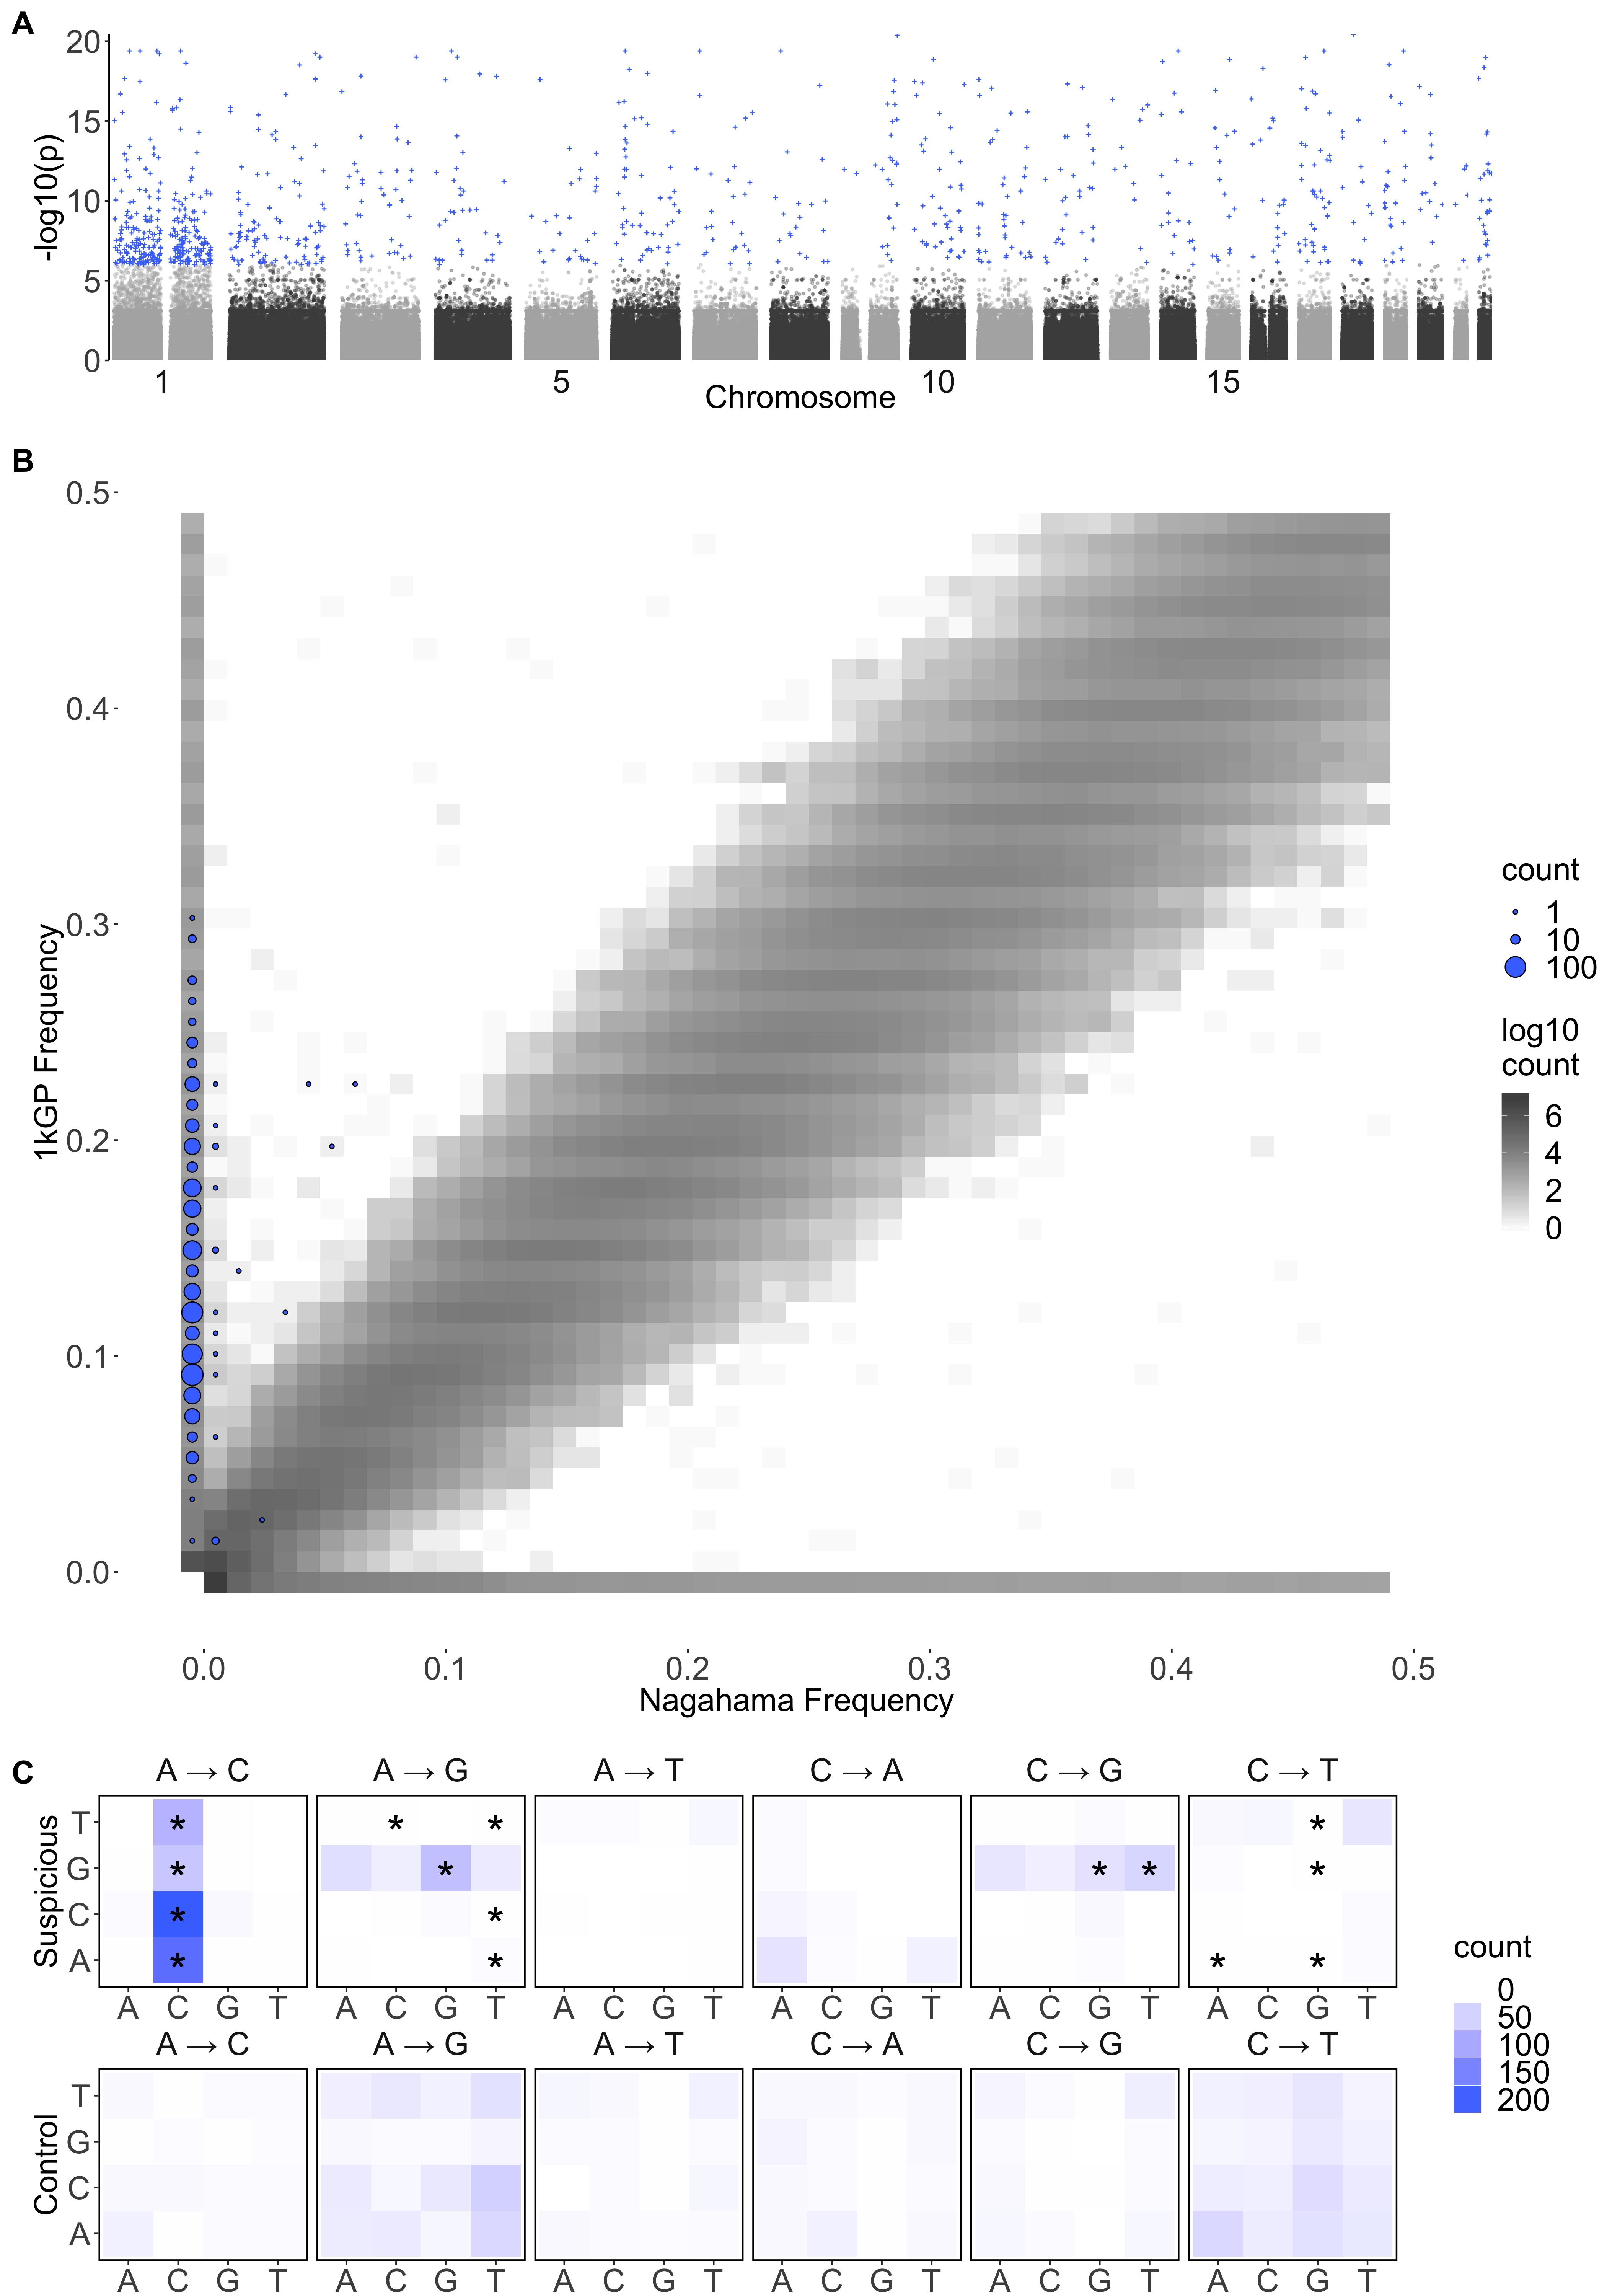
\includegraphics[width=\hsize,keepaspectratio]{../Figures/Figure1.jpg}}
\caption{
Suspicious mutations carried by individuals with low quality data have distinct mutational profiles, reproduce poorly across studies, and are distributed across the genome. 
\textbf{A} 
Genome wide association of the average quality of mapped bases $Q$ for the 104 Japanese individuals included in the 1000 Genomes Project. 
This GWAS identified $587\ \  p < 10^{-8}$ and $1034\ \ p < 10^{-6}$ SNPs that were associated to the average $Q$ of SNPs mapped for an individual.
The same analysis was performed independently for each of the populations in the 1000 Genomes Project.
\textbf{B} 
Joint frequency spectrum plot of the Japanese from the 1000 Genomes Project and a more recent Japanese dataset from Nagahama.
The size of blue dots are proportional to the number of variants that associate with $Q$ in the JPT. 
\textbf{C} 
Mutation spectrum of the 1034 variants that associated with $Q$ in the JPT($p < 10^{-6}$), compared to the proportional distribution of all SNPs.
The majority of the variants with significant associations to $Q$ have the *AC${\rightarrow}$*CC mutational pattern. 
There is also an enrichment in GA*${\rightarrow}$GG* and GC*${\rightarrow}$GG* mutations. 
These three enrichments can be summarized as G**${\rightarrow}$GG*. 
Stars ( * ) indicate a significant deviation from the expected mutational spectrum from all SNPs.
}
 \label{SFS}
\end{figure}


\section{Results}

			
\subsection{A peculiar mutational signature in Japan}			
	
Harris and Pritchard reported an excess of a 3-mer substitution patterns *AC${\rightarrow}$*CC in a portion of the Japanese individuals in the 1kGP \citep{Harris2017a}.
\todo{Our initial goal was to determine if this signature could be explained by population structure or technological error.}
While trying to follow up on this observation in a larger and more recent Japanese cohort from Nagahama, we did not find this particular signature.
When comparing the allele frequencies between the Japanese individuals from the 1kGP and this larger dataset, we observed a number of single nucleotide polymorphisms (SNPs) private to one of the two groups (Figure \ref{SFS}).
Given the similarity of the two populations, this strongly suggests a technical difference rather than a population structure effect.
These mismatches were maintained despite only considering sites that satisfied strict quality masks and Hardy-Weinberg equilibrium in both cohorts.

When mismatch sites are removed from the 1kGP data, the  *AC${\rightarrow}$*CC signal disappears (Figure \ref{SFS}). To identify possible technical reasons for the difference, we performed regressions of the prevalence of the  *AC${\rightarrow}$*CC mutational signature against different individual-level quality metrics provided by the 1kGP (see Figure \ref{PC1_Correlation}). 
The average quality of mapped bases  $Q$ per individual stood out as a strong correlate : Individuals with low $Q$ show elevated rates of the signature. 
Thus, sequences called from low-$Q$ data contain variants that reproduce poorly across studies and exhibit a particular mutational signature. 

\begin{figure}
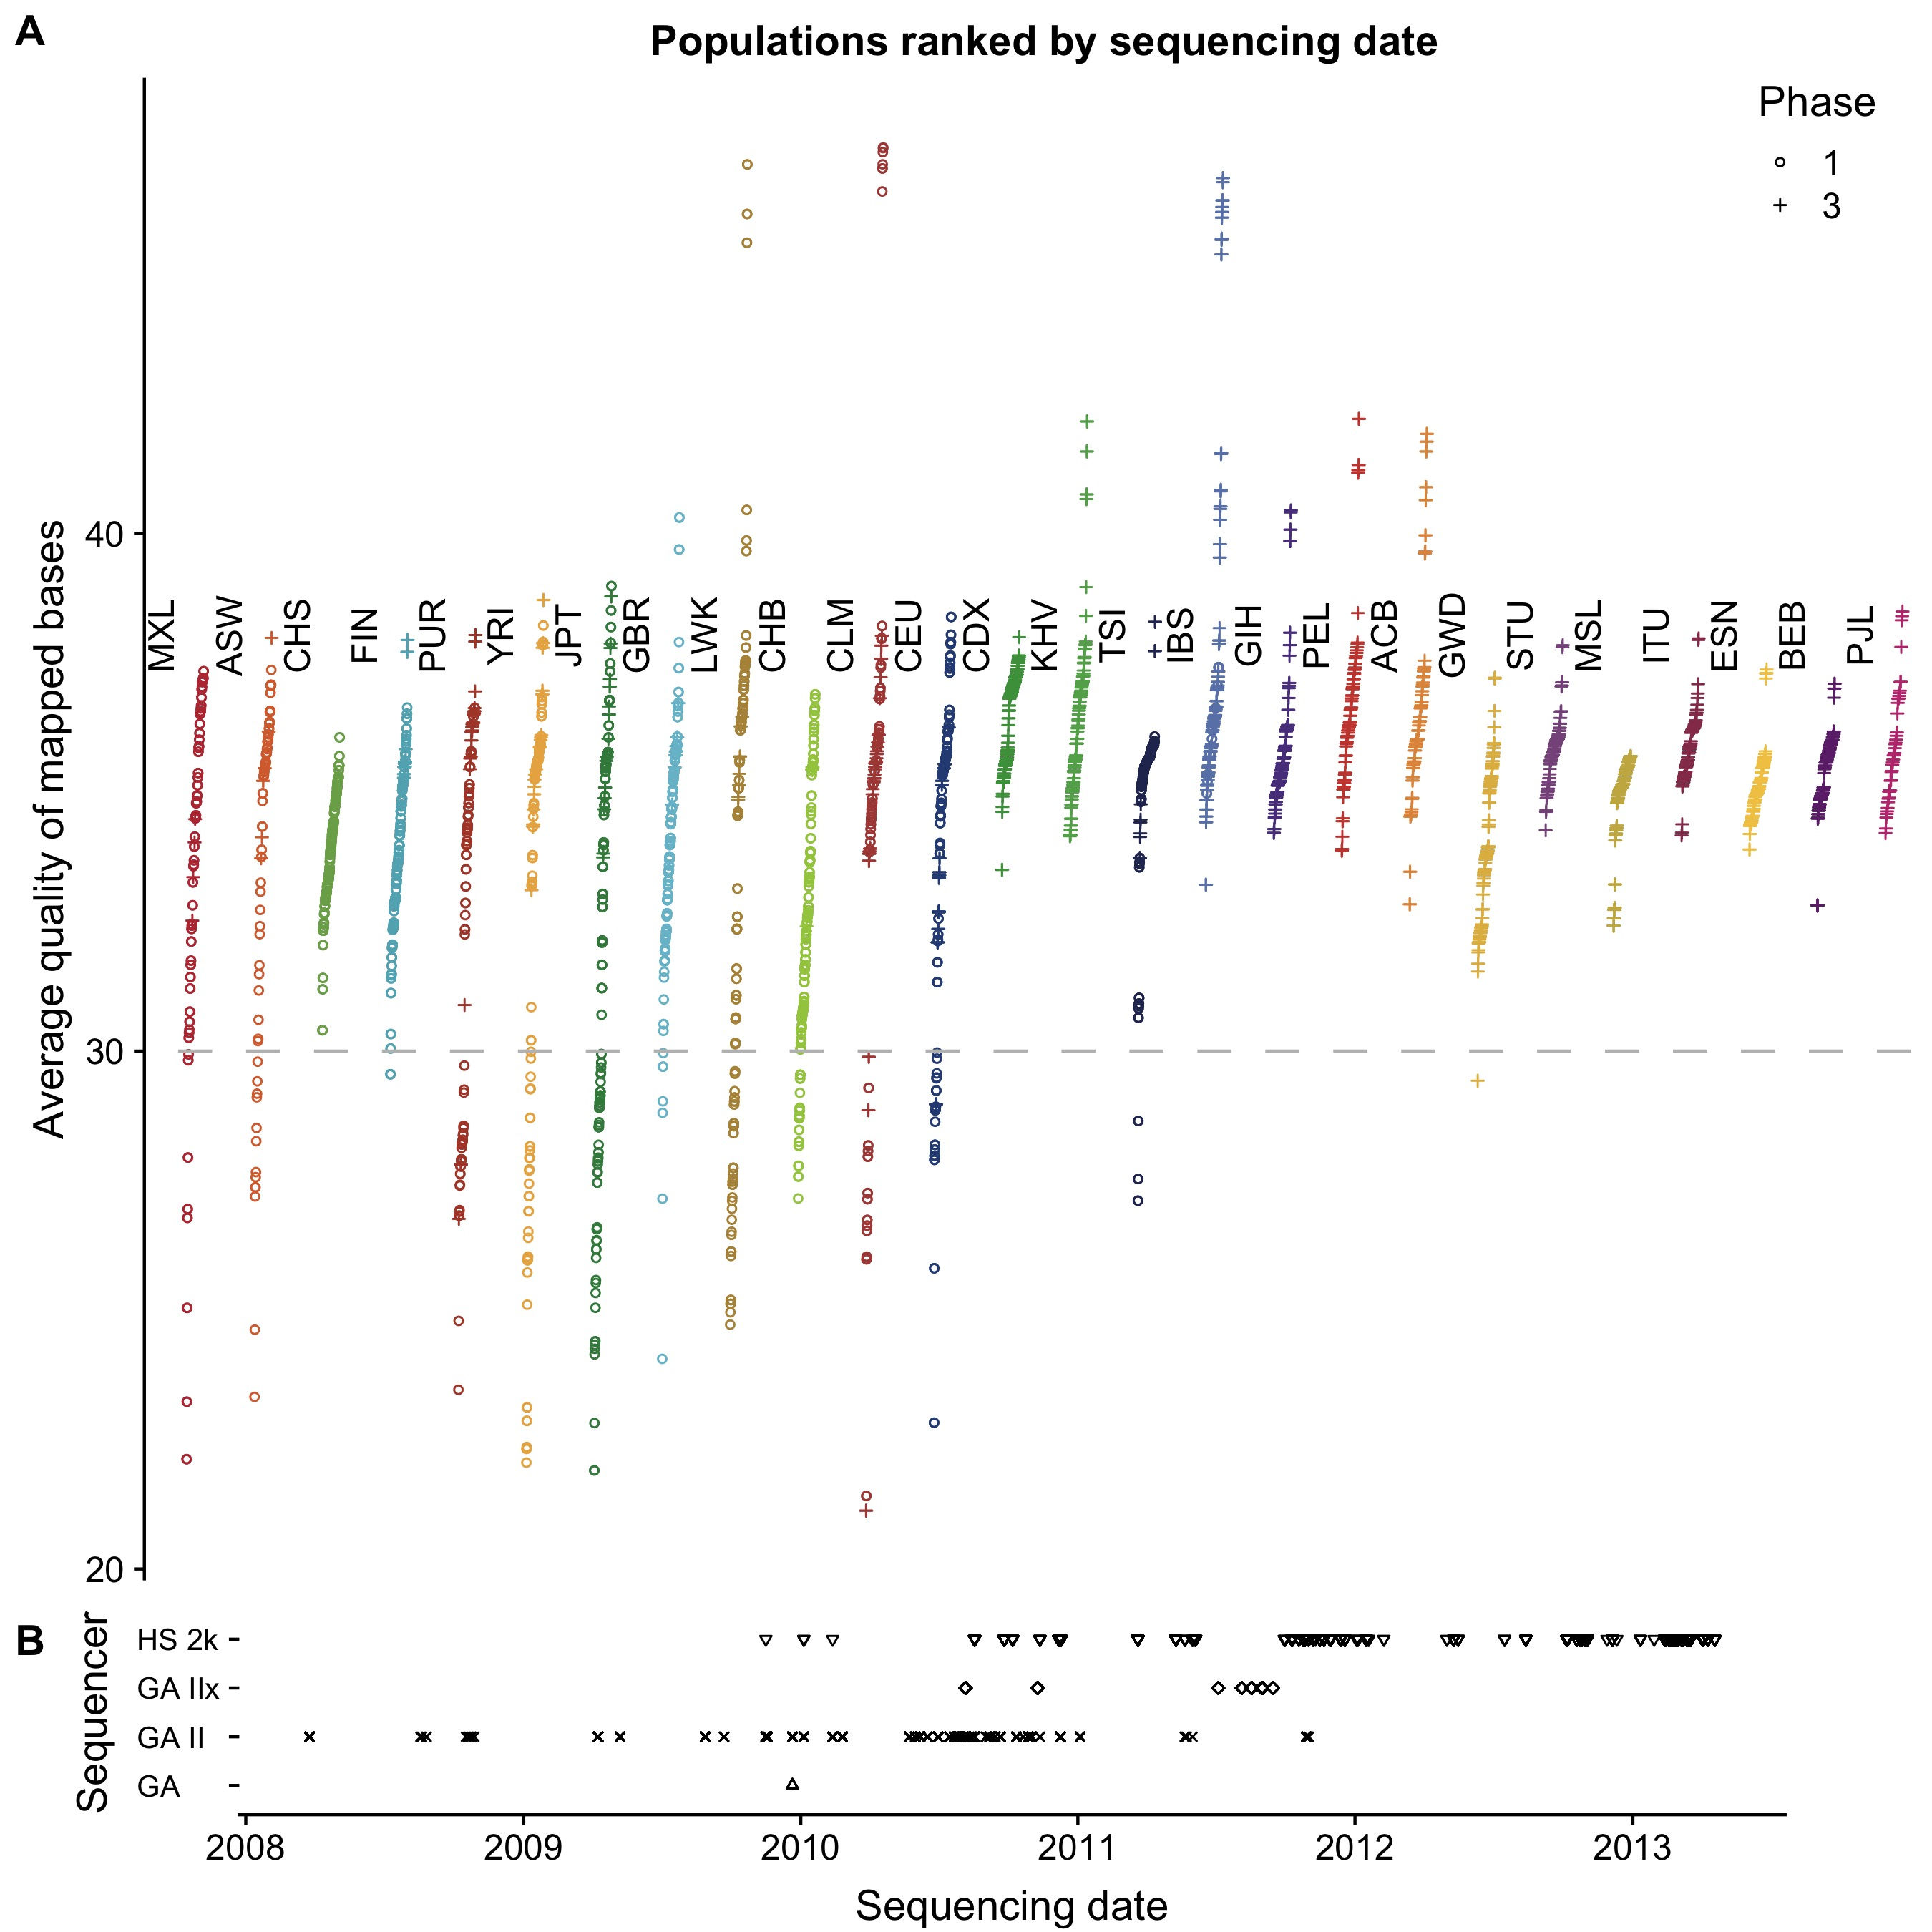
\includegraphics[width=0.95\hsize,keepaspectratio]{../Figures/MapQualOverTime.jpg}

\caption{Sampling and sequencing technologies over time in the 1000 Genomes Project.
\textbf{A} The average quality of mapped bases $Q$ for each individual per population included in the 1000 Genomes Project. 
 Populations are ranked by mean sequencing date (the earliest sequencing date was used for individuals with multiple dates). 
The shape indicates whether the individual belongs to Phase 1 or Phase 3 of the 1000 Genomes project. 
\textbf{B} Sequencing technologies used over the course of the 1000 Genomes Project.}
\label{MapQual}
\end{figure}

To identify SNPs that are likely to reproduce poorly across cohorts without having access to a second cohort, we performed an association study in the JPT for SNPs that associate strongly with low $Q$ (Figure \ref{SFS}).
Traditionally, genome wide association studies use genotypes as the independent variable. 
Here we perform a genotype conditional association test (GCAT), where genotypes are now the dependent variable that we attempt to predict using the continuous variable $Q$ as the independent variable \citep{song2015testing}.
We use logistic regression of the genotypes on $Q$ and identify 587 SNPs with $p < 10^{-8}$ and 1034 SNPs with $ p < 10^{-6}$. 
While identifying putative low-quality SNPs to exclude, using a higher $p$-value threshold increases the stringency of the filtering (i.e., excluding SNPs with $ p < 10^{-6}$ is more stringent than excluding SNPS with $p < 10^{-8}$). 
The variants that are associated to $Q$ have a significant enrichment in *AC${\rightarrow}$*CC mutations, GA*${\rightarrow}$GG*, and GC*${\rightarrow}$GG* mutations (Figure \ref{SFS}C).
These three enrichments can be summarized as an excess of G**${\rightarrow}$GG* in individuals with low $Q$.
Statistical significance of these enrichment is computed using a chi-squared test following \cite{Harris2017a}.

Thus, this mutational signal is heavily enriched in $Q$-associated SNPs, but residual signal remains in non-significant SNPs, presumably because many rare alleles found in individuals with low $Q$ remain unidentifiable using association techniques due to lack of power (Supplementary Figure \ref{histogram_of_sig_snps}).
The removal of individuals with $Q$ below 30 successfully removes the *AC${\rightarrow}$*CC signal, however other signals identified by Harris and Pritchard appear unchanged (Figure \ref{MutSpect}).
For population genetic analyses sensitive to the accumulation of rare variants, the removal of individuals with low $Q$ appears preferable to filtering specific low-quality SNPs. 
For other analyses where quality of imputation matters, identifying $Q$-associated variants may be preferable. 

\subsection{Identifying suspicious variants in the 1000 Genomes Project}
The distribution of $Q$ across 1kGP populations shows that many populations have distributions of $Q$ scores comparable to that of the JPT, especially populations sequenced in the phase 1 of the project: sequencing done in the early phases of the 1kGP was more variable and overall tended to include lower quality sequencing data (Figure \ref{MapQual} and Figure \ref{quality_by_center}).
This variability could result from evolving sequence platform and protocols or variation between sequencing centres. 
By 2011, older sequencing technologies were phased out, and methods became more consistent, resulting in higher and more uniform quality.

We therefore performed the same reverse GWAS approach in all populations independently, and similarly identified $Q$-associated SNPs in 23 of the 26 populations in the 1kGP, with the phase 1 populations being most affected, with on average four times as many significantly associated sites compared to the phase 3 populations.
Over 812 variants were independently associated to low $Q$ in at least two populations with $ p < 10^{-6}$ in each (Figure \ref{OverLap}).

To build a test statistic to represent the association across all populations simultaneously, we performed a simple logistic regression predicting genotype based on $Q$ with the logistic factor analysis (LFA) as an offset to account for population structure or Genotype-Conditional Association Test  (GCAT) as proposed by \citep{song2015testing}. 
We also considered two alternative approaches to account for confounders, namely using the leading five  principal components, and using population membership as covariates. 
These models were broadly consistent (See Figure \ref{CompareModel}).

This method identifies a total of 24,390 variants associated to $Q$ distributed across the genome with 15,270 passing the 1kGP strict mask filter (Figures \ref{NRS_Manhattan},\ref{NRI_Manhattan}, \ref{RS_Manhattan}, and \ref{RI_Manhattan}). Most analyses below focus on the 15,270 variants satisfying the strict mask, since these variants are unlikely to be filtered by standard pipelines.
To account for the large number of tests, we used a two-stage Benjamini \& Hochberg step-up FDR-controlling procedure to adjust the p-values using a nominal Type-I error rate $\alpha = 0.01$ \citep{Benjamini2006}. 
We tested SNPs, INDELs and repetitive regions separately as they may have different error rates (Table \ref{sigTable}).
Lists of $Q$-associated variants and individuals with low $Q$ are provided in Supplementary Data.

$Q$-associated variants are distributed across the genome, with chromosome 1 showing an excess of such variants, and other chromosomes being relatively uniform (Figure \ref{CountPerChrom}).
At a 10kb scale, we also see rather uniform distribution with a small number of regions showing an enrichment for such variants (Figure \ref{VariantDensity}).
An outlying 10kb region in chromosome 17 (bases : 22,020,000 to  22,030,000) has 35 $Q$-associated variants.
Distribution of association statistics in this region is provided in Figure \ref{Top10}.
By contrast, variants that do not pass the 1kGP strict mask are more unevenly distributed across the genome (Figure \ref{VariantDensity}).
\todo{The mutational 3-mer substitution patterns of this list of variants is similar to the signature identified in the single population test of the 1kGP JPT in that there is an enrichment in *AC${\rightarrow}$*CC.
However, another enrichment profile is significantly enriched : TAT${\rightarrow}$TTT, TCT${\rightarrow}$TTT and ACA${\rightarrow}$AAA (reverse complement : TGT${\rightarrow}$TTT). These three enrichments can be summarized as T*T${\rightarrow}$TTT.}

\todo{A recent publication by Mafessoni et al. also identified a batch effect in the 1kGP using a different method.
We find that only 10\% of the variants they identified are in our list of suspicious variants and have correlated p-values to those identified using the GCAT method \ref{Mafessoni_MutSpect}.
Moreover, the variants they identified are not enriched in the mutational spectra described above \ref{Mafessoni_MutSpect}. }


\begin{table}[h!]
\centering
\begin{tabular}{l  r r r}
                      & {Repeat}  & {Non-Repeat}   & {Total}    \\ \hline
{SNP}  & 3,369 \textcolor{gray}{0.53\textperthousand} & 11,059 \textcolor{gray}{0.56\textperthousand} & 14,428\\  
{INDEL} & 181 \textcolor{gray}{0.3\textperthousand} & 657 \textcolor{gray}{0.66\textperthousand} & 838\\ \hline
{Total} & 3,550 & 11,716 & 15,270\\
\end{tabular}
\caption{Number of statistically significant variants  passing the 1000 Genomes Project strict mask per category. 
Variants that are flagged by the 1000 Genomes Project nested repeat mask file were analyzed separately for FDR calculation. SNPs and INDELs were also analyzed separately.
A total of 15,270 are statistically significantly associated to $Q$. 
\todo{The grey text is the proportion of significant associations per category.}
The number of variants included in the analysis for SNPs, SNPs in repeat regions, INDELs and INDELs in repeat regions are  19,846,786, 6,312,620, 1,770,315 and 586,342 respectively.}
\label{sigTable}
\end{table}

\subsection{Cell line or technical artifact}

In 2017, Lan et al. resequenced 83 Han Chinese individuals from the 1kGP \citep{Lan2017}. To assess consistency between the two datasets, we consider consistency of genotype calls for $Q$-associated variants that are predicted to be polymorphic in these 83 individuals according to the 1kGP.
Among the 296 such variants that were $Q$-associated in the CHB or CHS, only 6 are present in the resequenced data (Figure \ref{90HanSFS}). 
\todo{This is more than the number of false positives predicted by our nominal false discovery rate of $\alpha = 0.01$ ($0.01 \times 296 = 2.96$)}. 
Thus a small number of variants associated to $Q$ are present in the population but with somewhat biased genotypes. 


We did a similar analysis using all variants identified in the GCAT model (rather than only variants significantly associated to $Q$ within the CHB and CHS). 
Of the 15,270 $Q$-associated variants identified globally, 6,307 are polymorphic in the 1kGP for the 83 resequenced individuals  (See Figure \ref{90HanSFS_full}).
From this subset, only 1,139 (or 18\%) are present in the resequenced data.
The allele frequencies of these variants are nearly identical between datasets suggesting that among these 83 individuals, these variants are properly genotyped in the 1kGP.
\todo{Some mutational signatures are heterogenous where not all suspicious variants are completely spurious in all individuals or populations. 
Some mutational signatures reproduce across cohorts, whereas others do not and may be due to the different sequencing platforms used.}
There are 5 variants that show differing frequencies between both datasets that are likely explained by biased genotypes.
The vast majority of polymorphisms associated with $Q$ are not present at all in the resequencing dataset, supporting sequencing rather than cell line artifacts.

Among the 15,270 $Q$-associated variants, 613 are present on Illumina's Omni 2.5 chip (See Figure \ref{Omni}). 
These are likely among the small number of variants that are present in the data but exhibit biased genotyping in 1kGP. 

\subsection{Suspicious variants impact modern genomics analyses}

State of the art imputation servers use a combination of many databases including some that are not freely available.
From the perspective of researchers, they act as black-box imputation machines that take observed genotypes as input and return imputed genotypes.  

To investigate whether suspicious calls from the 1kGP are imputed into genotyping studies, we submitted genotype data for the first two chromosomes of the 1kGP genotype data to the Michigan Imputation Server.
We found that all of the variants associated with $Q$ were imputed back in the samples.
This suggests that the imputation reference panel still includes individuals with low $Q$, and the dubious variants will be imputed in individuals who most closely match the low-quality individual.
These $Q$-associated variants could also compromise the imputation of nearby real-variants causing not only improper imputation, but also false negatives for real variants.

We searched the literature for any GWAS that might have reported these $Q$-associated variants as being significantly associated with some biological trait, even though there is no particular reason for these variants to be associated with phenotypes.
The NHGRI-EBI Catalog of published genome-wide association studies identified seventeen recent publications that had reported these variants as close to or above the genome-wide significant threshold (Table \ref{gwasTable}).
Some of these publications noted that these variants were not flanked by linkage disequilibrium peaks \citep{Mandage2017}.
Indeed, we expect a large number of these variants to be filtered out by some quality controls like the Hardy-Weinberg  equilibrium test.
However, the fact that some of these variants are not removed and that the great majority of these variants are missing from higher quality datasets means that these $Q$-associated variants should be flagged for removal to avoid spurious association.

Eleven of these studies included the 1kGP in their reference panel for imputation \citep{xu2012genome, lutz2015genome, park2015mercapturic, astle2016allelic, herold2016family,  suhre2017connecting, lopez2017genome, tian2017genome,  spracklen2017association,  nagy2017exploration, gao2018genome} and another used the 1kGP sequence data and cell lines directly \citep{Mandage2017}.
One study used an in-house reference panel for imputation \citep{nishida2018key}, two studies genotyped individuals and imputed the data using the HapMap II as a reference  database for imputation \citep{Kraja2011, Ebejer2013} and two studies used genotyping chip data \citep{yucesoy2015genome, ellinghaus2016analysis}. 

These articles used a variety of strict quality filters, including Hardy-Weinberg equilibrium test, deviations in expected allele frequency and sequencing data quality thresholds.
They also removed rare alleles and alleles with high degrees of missingness.
Despite using state-of-the-art quality controls, these variants managed not only to be imputed onto real genotype data, but they also reached genome wide significance for association with biological traits.

These associations are not necessarily incorrect -- a weak but significant bias in imputation may still result in a correct associations.
To distinguish between variants with weak but significant association with $Q$ from variants with strong biases, we distinguished between variants where the allele frequency difference between individuals with low- and high-$Q$ is larger than a factor of two (which naturally separates two clusters of variants on Figure \ref{90HanSFS_full}).
The majority (92.7\%) of the $Q$-associated variants are strongly biased in that they are more than twice as frequent in individuals with low-$Q$ compared to high-$Q$ data.
By contrast, most $Q$-associated variants reported in the GWAS catalogue had weak bias (See Figure \ref{Pub_30}), with three exceptions.
One study reports associations with seven $Q$-associated variants that we find to be highly biased \citep{Mandage2017}. 
That study considered copy number of Epstein-Barr virus (EBV) sequence in the 1kGP as a phenotype. 
\todo{It is plausible that the EBV copy number phenotype is sensitive to mapping and in this study, may be confounded by the same technical artefacts that lead to biased SNP calling.}



\begin{table}[h!]
\begin{tabular}{l l l r r r}
  {Pubmed ID}  & {Disease/Trait} & {rsID} & \multicolumn{1}{p{1cm}}{\centering GWAS \\ -$\log_{10} p$} & \multicolumn{1}{p{1.5cm}}{\centering $Q$\\-$\log_{10} p$\\(adjusted)}      \\ \hline
28654678 & EBV copy number in & rs201761909 & 5.7 & 78.11\\
	&   lymphoblastoid cell lines	&  	rs201130852 & 5.05 & 72.28\\
	& 	&  	rs201255786 & 5.7 & 68.97\\
	& 	&  	rs200655768 & 6.52 & 66.67\\
	& 	&  	rs184202621 & 5.52 & 60.45\\
	& 	& 	rs80274284 & 6 & 56.15\\
	& 	& 	rs200699422 & 5.3 & 7.43\\
23527680 & \multicolumn{1}{p{3cm}}{\raggedright ADHD\textsuperscript{\dag}} & rs6057648 & 5.4 & 20.5\\
28928442 & \multicolumn{1}{p{3cm}}{\raggedright Cold sores} & rs201471471 & 6.52 & 7.87\\
26053186 & \multicolumn{1}{p{3cm}}{\raggedright HMPMA\textsuperscript{\ddag} levels in smokers} & rs60136336 & 5.7 & 2.25\\ \hline
\textcolor{gray}{28270201} & \multicolumn{1}{p{3cm}}{\raggedright \textcolor{gray}{HDL cholesterol}} & \textcolor{gray}{rs453755} & \textcolor{gray}{7.52} & \textcolor{gray}{5.29}\\
\textcolor{gray}{23023329} & \multicolumn{1}{p{3cm}}{\raggedright \textcolor{gray}{Prostate cancer}} & \textcolor{gray}{rs103294} & \textcolor{gray}{*15.3} & \textcolor{gray}{4.32}\\
\textcolor{gray}{28334899} & \multicolumn{1}{p{3cm}}{\raggedright \textcolor{gray}{HDL cholesterol}} & \textcolor{gray}{rs103294} & \textcolor{gray}{*29.3} & \textcolor{gray}{4.32}\\
\textcolor{gray}{28240269} & \multicolumn{1}{p{3cm}}{\raggedright \textcolor{gray}{Blood protein levels}} & \textcolor{gray}{rs103294} & \textcolor{gray}{*72.7} & \textcolor{gray}{4.32}\\
\textcolor{gray}{27863252} & \multicolumn{1}{p{3cm}}{\raggedright \textcolor{gray}{High light scatter\\reticulocyte count}} & \textcolor{gray}{rs3794738} & \textcolor{gray}{*13.15} & \textcolor{gray}{3.73}\\
\textcolor{gray}{29534301} & \multicolumn{1}{p{3cm}}{\raggedright \textcolor{gray}{Response to\\hepatitis B vaccine}} & \textcolor{gray}{rs9273062} & \textcolor{gray}{*9.7} & \textcolor{gray}{3.36}\\
\textcolor{gray}{21386085} & \multicolumn{1}{p{3cm}}{\raggedright \textcolor{gray}{Metabolic syndrome}}  & \textcolor{gray}{rs301} & \textcolor{gray}{*10.52} & \textcolor{gray}{3.02}\\
\textcolor{gray}{26830138} & \multicolumn{1}{p{3cm}}{\raggedright \textcolor{gray}{Alzheimer disease\\and age of onset}} & \textcolor{gray}{rs77894924} & \textcolor{gray}{6.7} & \textcolor{gray}{2.77}\\
\textcolor{gray}{29617998} & \multicolumn{1}{p{3cm}}{\raggedright \textcolor{gray}{Intraocular pressure}} & \textcolor{gray}{rs4963156} & \textcolor{gray}{*22.4} & \textcolor{gray}{2.52}\\
\textcolor{gray}{28698626} & \multicolumn{1}{p{3cm}}{\raggedright \textcolor{gray}{Immunoglobulin A vasculitis}} & \textcolor{gray}{rs11015915} & \textcolor{gray}{5.05} & \textcolor{gray}{2.45}\\
\textcolor{gray}{26974007} & \multicolumn{1}{p{3cm}}{\raggedright \textcolor{gray}{Chronic inflammatory diseases}} & \textcolor{gray}{rs3124998} & \textcolor{gray}{*8.05} & \textcolor{gray}{2.33}\\
\textcolor{gray}{26634245} & \multicolumn{1}{p{3cm}}{\raggedright \textcolor{gray}{Post bronchodilator}} & \textcolor{gray}{rs451000} & \textcolor{gray}{6} & \textcolor{gray}{2.28}\\
 	& \multicolumn{1}{p{3cm}}{\raggedright \textcolor{gray}{FEV1/FVC ratio}} 	& 	\textcolor{gray}{rs443874} & \textcolor{gray}{5.3} & \textcolor{gray}{2.26}\\
	& 	&	\textcolor{gray}{rs400942} & \textcolor{gray}{6} & \textcolor{gray}{2.2}\\
\textcolor{gray}{25918132} & \multicolumn{1}{p{3cm}}{\raggedright \textcolor{gray}{Diisocyanate-induced asthma}} & \textcolor{gray}{rs76780579} & \textcolor{gray}{6} & \textcolor{gray}{2.09}\\

 \hline
\end{tabular}
\caption{Recent publications that reported $Q$-associated variants as close to or above the genome-wide significant threshold. The variants reaching genome wide significance have a star ( * ). The black text colour indicates that this variant is twice as frequent in individuals with $Q$ < 30, grey text colour indicates that these variants are less than twice as frequent in individuals with $Q$ < 30 (See Figure \ref{Pub_30}).
\textsuperscript{\dag} Attention deficit hyperactivity disorder. 
\textsuperscript{\ddag} 3-hydroxy-1-methylpropylmercapturic acid.
}
\label{gwasTable}
\end{table}

\section{Discussion}

The variants identified in this study are likely to be technical artifacts from legacy technologies.
Different sequencing technologies will have different error profiles. 
A report comparing the Genome Analyzer II (GAII) to the Illumina HiSeq found that the GAII had much higher rates of reads below a quality score of 30 \citep{Minoche2011} with, for instance, different patterns of quality decrease along reads. 
Differences in read quality and error profiles in turn require different calling pipelines.
 
To pinpoint the precise technical source of the discrepancy would require further forensic inquiries into the details of the heterogeneous sample preparation and data processing pipelines used throughout the 1kGP. Given the progress in sequencing and calling that occurred since the early phases of the 1kGP (Figure \ref{MapQual}), it is likely that the source of these biases is not longer being actively introduced in recent sequence data.

However, because the 1kGP data is widely used as a reference database, these variants are still being imputed onto new genotype data and can then impact association studies for a variety of phenotypes. Even though significant association of a variant with a quality metric is not in itself an indication that the variant is spurious, we would recommend to carefully examine GWAS associations for such variants, e.g. by repeating the analysis without the 1kGP as part of the imputation panel. 

For analyses where individual variants cannot be examined individually (mutation profiles, distributions of allele frequencies, polygenic risk scores), we would recommend to simply discard the $Q$-associated SNPs or the individuals with $Q<30$ (lists of such variants and sample IDs are provided in the Supplementary Data). We also recommend that imputation servers discard individuals with low Q (or at least provide the option of performing the imputation without). Given the value of freely accessible data, resequencing individuals with low Q would  also likely be a worthwhile investment for the community. 

\section{Conclusion}

On a technical front, we were surprised that strong association between variants and technical covariates in the 1kGP project had not been identified before. 
The genome-wide logistic regression analysis of genotype on quality metric is straightforward, and should probably be a standard in a variety of -omics studies. The logistic factor analysis is more computationally demanding but produces more robust results \citep{song2015testing}. Both approaches produce comparable results.  

More generally, to improve the quality of genomic reference datasets, we can proceed by addition of new and better data and by better curation of existing data.
Given rapid technological progress, the focus of genomic research is naturally on the data generation side. 
However, cleaning up existing databases is also important to avoid generating spurious results. 
The present findings suggest that a substantial fraction of data from the final release of the 1kGP project is overdue for retirement or re-sequencing.


\section{Methods}
\subsection{Code and data availability}
Since this data is primarily performed using publicly available data, we provide fully reproducible and publicly available on \href{https://github.com/LukeAndersonTrocme/LegacyData}{GitHub}.
This repository includes scripts used for data download, processing, analysis and plotting.
%Supplementary data as well as preprocessed data for plotting are also available on GitHub.

\subsection{Metadata}
The metadata used in this analysis was compiled from each of the index files from the 1kGP file system. 
Average quality of mapped bases $Q$ per sample was obtained from the BAS files associated with each alignment file.
Each BAS file has metadata regarding each sequencing event for each sample. 
If a sample was sequenced more than once, we took the average of each $Q$ score from each sequencing instance. 
The submission dates and sequencing centres for each sample in the analysis was available in the sequence index files.

\subsection{Quality Controls}
For the mutation spectrum analysis, we reproduced the quality control and data filtering pipelines used by Harris et al. as they applied the current state of the art quality thresholds to remove questionable sequences for detecting population level differences. 
Several mask files were applied to remove regions of the genome that might be lower quality, or might have very different mutation rates or base pair complexity compared to the rest of the genome. 
The 1kGP strict mask was used to remove low quality regions of the genome, highly conserved regions were removed using the phastCons100way mask file and highly repetitive regions were removed using the NestedRepeats mask file from RepeatMasker.
Furthermore, only sites with missingness below 0.01, MAF less than 0.1, and MAF greater than 0.9 were considered.
In total, 7,786,023 diallelic autosomal variants passed our quality controls for the mutation spectrum analysis.
We calculated the mutation spectrum of base pair triplets for the list of significant variants for the JPT population using a similar method as described in  \citep{Harris2017a}.

For the reverse GWAS, the only filtration used was the application of an minor and major allele frequency cutoff of 0.000599 (removing singletons, doubletons and tripletons) resulting in a total of S=28,516,063 variants included in the test. 
We also used the NestedRepeats mask file to flag variants inside repetitive regions as these were analyzed separately for false discovery rate estimation.
Variants flagged by the 1kGP strict mask are included in the association test and included in the FDR adjustment. 
These variants are only removed after the FDR and excluded from downstream discussion of error patterns, since most population genetics analyses use the strict mask as a filter, and we expect to find problematic variants in filtered regions.

\subsection{Testing the association of quality to genotype}
When conducting a statistical analysis of population genetics data, we must account for population structure. In a typical GWAS, we are interested in modelling the phenotype as a function of the genotype. 
Here we have the opposite situation, where the quantitative variable ($Q$) is used as an explanatory variable. 
So we consider models where the genotype $y$ is a function of an expected frequency $\pi_{si},$ based on population structure, and $Q$. 
The null model is 
\begin{align} \label{lfa_basic}
y_{si} \mid \pi_{si}  &\sim Binomial\big( 2, \pi_{si} \big).
\end{align} 
The expected frequency for a SNP $s$ and individual $i$ can be estimated using principal component analysis, categorical population labels, or logistic factor analysis \citep{song2015testing}. The alternative model then takes in $Q$ as a covariate: 

\begin{align}\label{gcat_basic}
 y_{si} \mid q_i, \boldsymbol{h}^{(i)} &\sim Binomial\bigg( 2, \logit^{-1}\Big(\logit(\pi_{si}) + \beta_s q_i\Big) \bigg).
\end{align} 

Under the null hypothesis the slope coefficient $\beta_s$ is zero and Model \eqref{gcat_basic} reduces to Model \eqref{lfa_basic}. 
$\beta_s$ denotes the association to average quality of mapped bases $Q$ to genotype $y_{s}$. 
To test the null hypothesis, we use the generalized likelihood ratio test statistic, whose deviance is a measure of the marginal importance of adding $Q$ in the model. 
The deviance test statistic under the null model is approximately chi-square distributed with one degrees of freedom.

We run a total of $S$ regressions, where $S$ is the total number of genomic loci. Given the large number of tests, the large proportion of expected null hypotheses and the positive dependencies across the genome, we used the two-stage Benjamini \& Hochberg step-up FDR-controlling procedure to adjust the \textit{p}-values \citep{Benjamini2006}.
By using a nominal Type-I error rate $\alpha = 0.01$, a total of 15,270 variants were found to be statistically significance. 
See Supplementary Data for a list of variants and adjusted \textit{p}-values.

\subsection{Individual-specific allele frequency}
Examples of models that are widely used to account population structure include the Balding-Nichols model \citep{balding1995method}, and the Pritchard- Stephens-Donnelly model \citep{pritchard2000inference}. 
These and several other similar models used in GWAS studies can be understood in terms of the following matrix factorization. 
\begin{align}
\mathbf{L }= \mathbf{AH}
\end{align} 
where the $i^\text{th}$ column ($\boldsymbol{h}^{(i)}$) of the $K \times I$ matrix $\mathbf{H}$ encodes the population structure of the $i^\text{th}$ individual and the $s^\text{th}$ row of the $S \times K$ matrix $\mathbf{A}$ determines how that structure is manifested in SNP $s$. 
When Hardy-Weinberg equilibrium holds, observed genotype can be assumed to be generated by the following Binomial model.
\begin{align} \label{lfa}
y_{si} \mid \pi_{si}  &\sim Binomial\big( 2, \pi_{si} \big) 
\end{align} 
for $s=1\hdots S$ and $i=i,\cdots, I$, where $y_{si} \in \{0,1,2\}$ and $logit(\pi_{si})$ is the $(s,i)$ element of the matrix $\mathbf{L}$ such that  $\pi_{si}$ is the individual-specific allele frequency.

To test whether quality is associated to genotype while adjusting for population structure, we performed the Genotype-Conditional Association Test  (GCAT) proposed by \citep{song2015testing}.
The GCAT is a regression approach that assumes the following model.
\begin{align}\label{gcat}
 y_{si} \mid q_i, \boldsymbol{h}^{(i)} &\sim Binomial\bigg( 2, logit^{-1}\Big( \sum_{k=0}^{K} a_{sk} h_{ki} + \beta_s q_i\Big) \bigg)
\end{align} 
for $s=1\hdots S$ and $i=i,\cdots, I$  ($S = 28,516,063$ and $I = 2,504$) and where $\hat{h}_{0i}=1$ so that $a_{s0}$ is the intercept term and $logit(\pi_{si})=\sum_{k=0}^{K} a_{sk} h_{ki}$. 
The vectors $\boldsymbol{h}^{i}$ of the matrix $\mathbf{H}$ are unobserved but can be estimated using Logistic Factor Analysis (LFA) \citep{song2015testing} and are therefore used directly in the model. 
We approximated the population structure using $K=5$ latent components from a subsampled genotype matrix consisting of $M = 2,306,130$ SNPs (we picked SNPs from the 1kGP OMNI 2.5). 
To avoid possible biases in computing PCA from the biased variants, we considered the genotype matrix $L$ obtained by downsampling 1kGP variants the positions from the OMNI 2.5M chip.

\subsection{Imputation}
Using the Michigan Imputation Server, we imputed the genotype data from 1kGP for chromosomes 1 and 2.
We used the genotyped data from the 1kGP Omni 2.5M chip genotype data.
The VCF file returned from the server was then downloaded and used to search for the number of significant variants successfully imputed. 

\section{Acknowledgments}
We would like to thank Kelly Harris for sharing her mutation spectrum scripts.
We would also like to thank the members of the Gravel lab for their help with coding and useful discussions.


\bibliography{Legacy}

\clearpage
\section{Supplementary Figures}
\renewcommand{\thefigure}{S\arabic{figure}}
\setcounter{figure}{0}   	

\begin{figure}
\centering
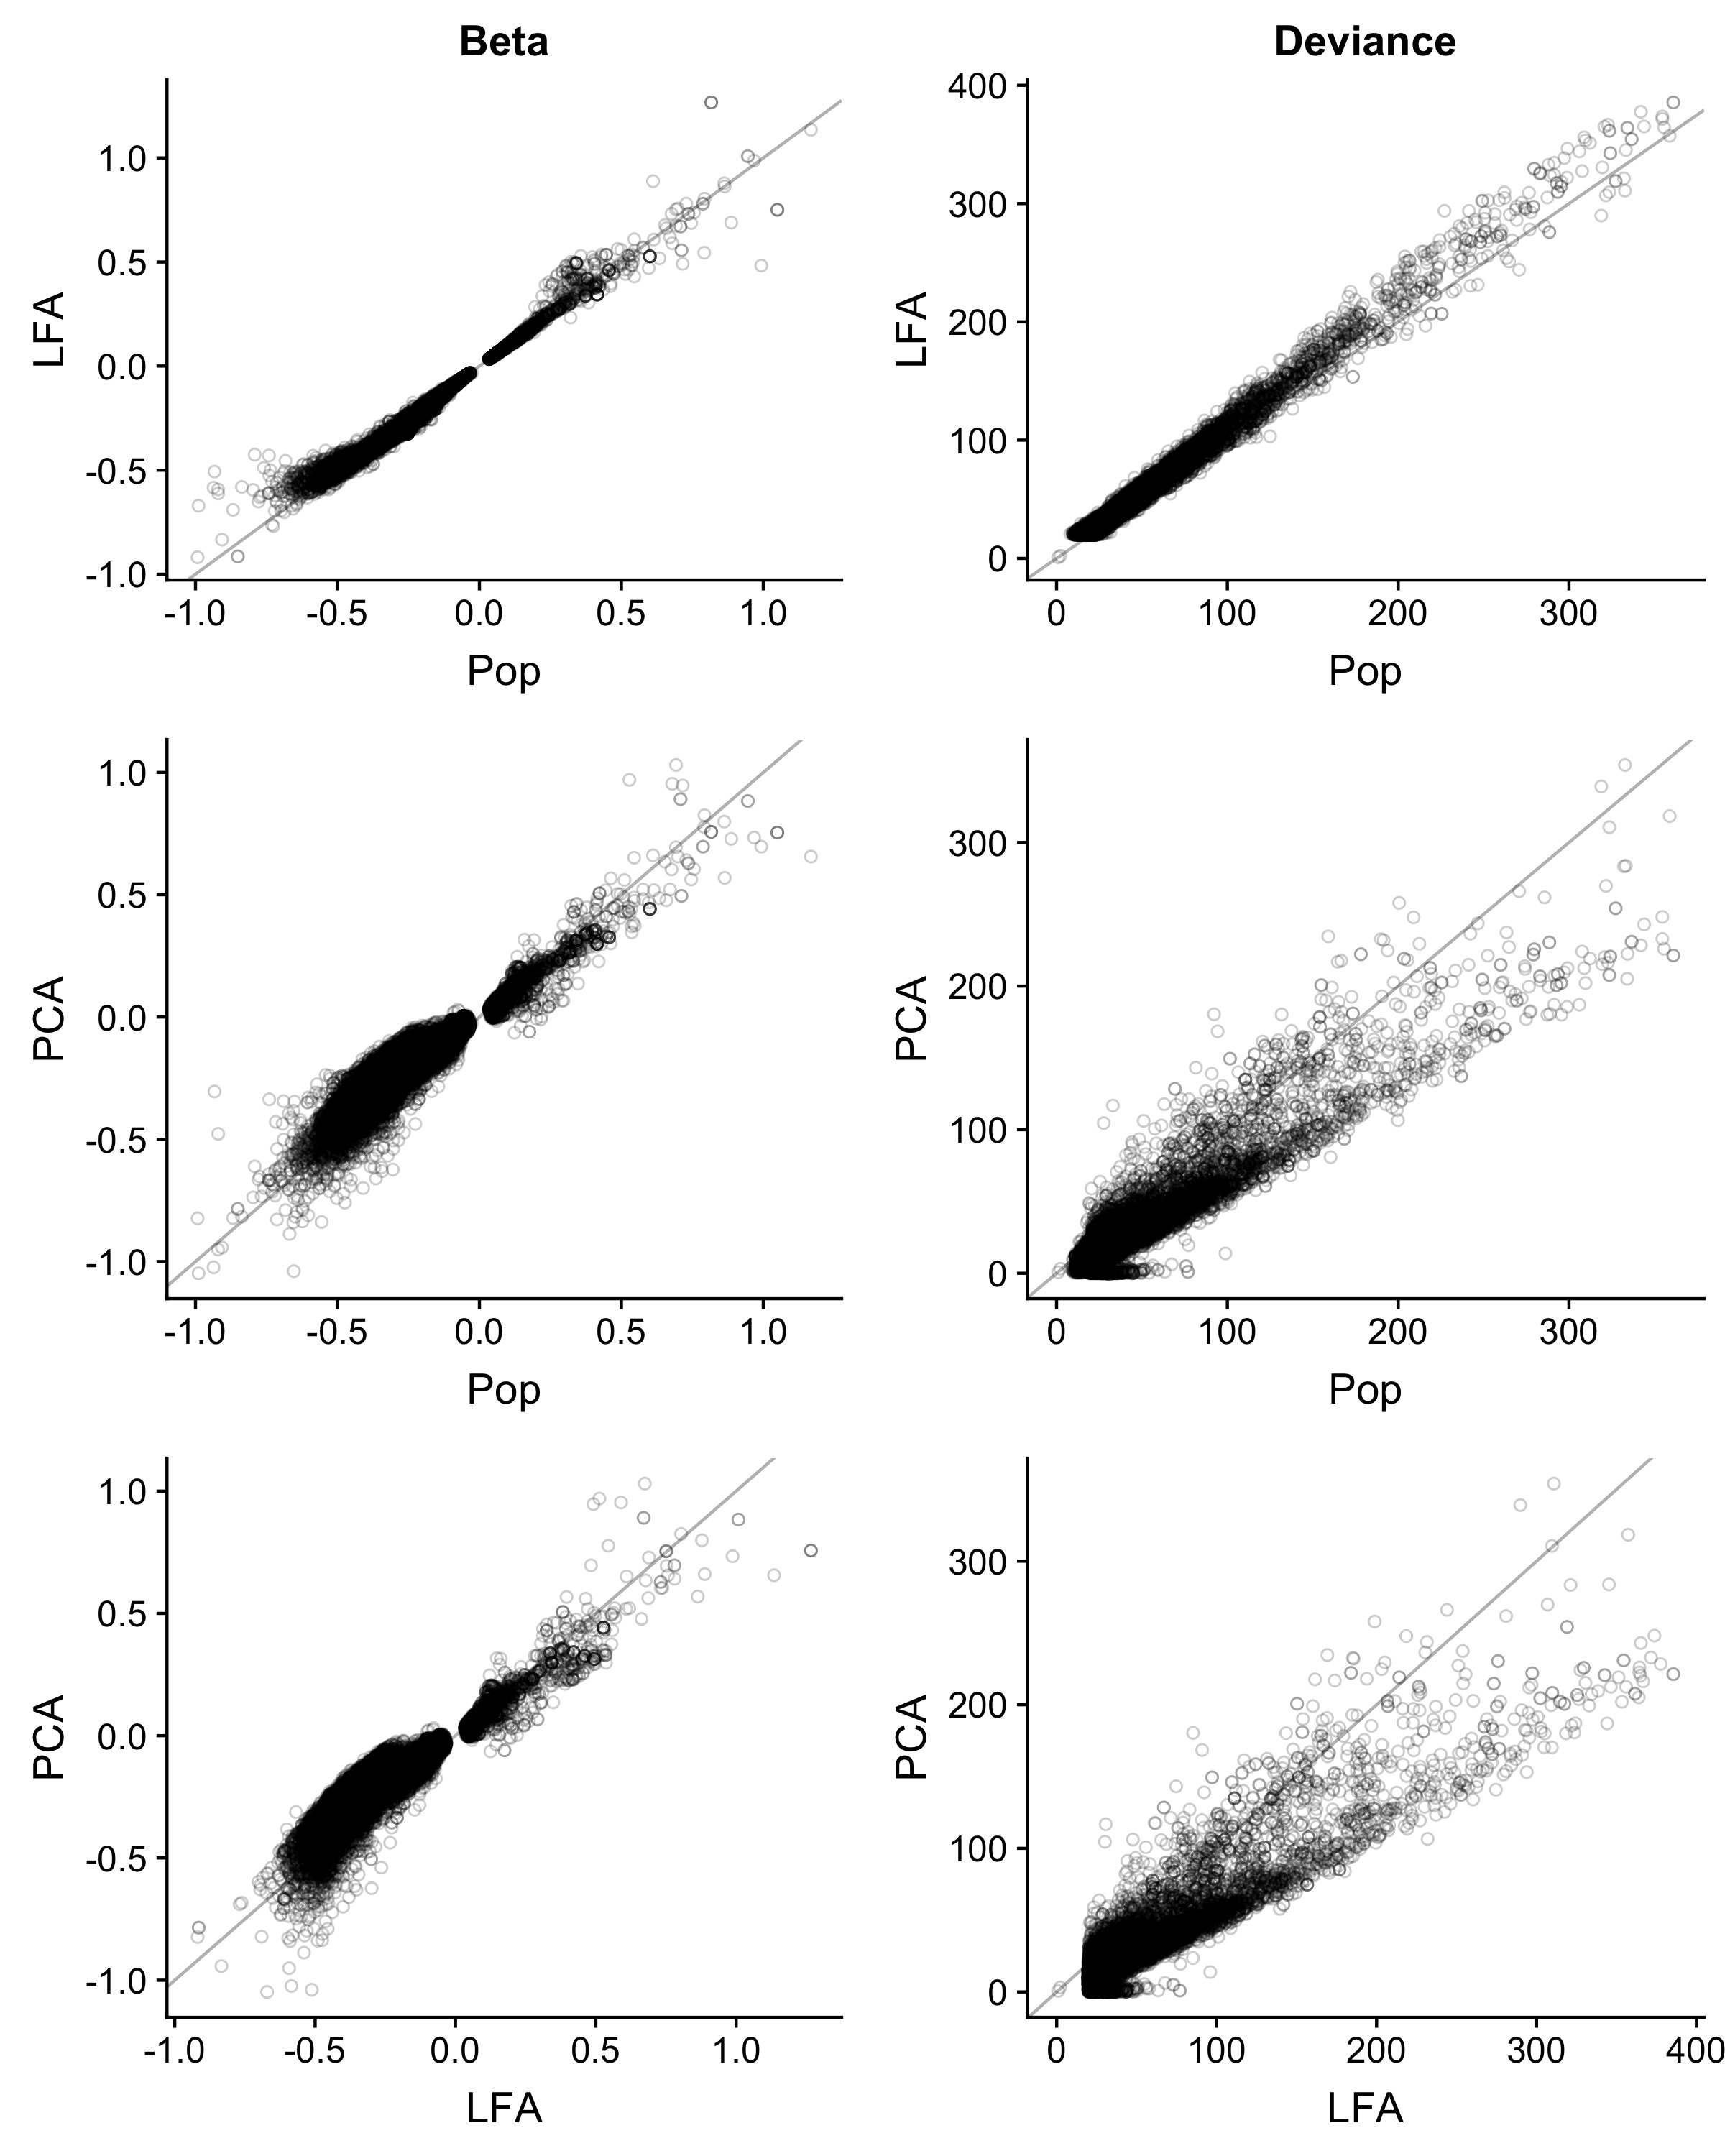
\includegraphics[width=13cm,keepaspectratio]{../Figures/fits_Significant_Positions_CompareModels.jpg}
\caption{Comparison of three logistic regression models for testing association to $Q$.
These methods model each genotype as a logistic function using principal components (PC), Population membership (Pop) or LFA as an offset.
In these plots we are comparing the deviance from the null model in the 15,270 variants identified using the LFA model.}  
\label{CompareModel}
\end{figure}

\begin{figure}
\centering
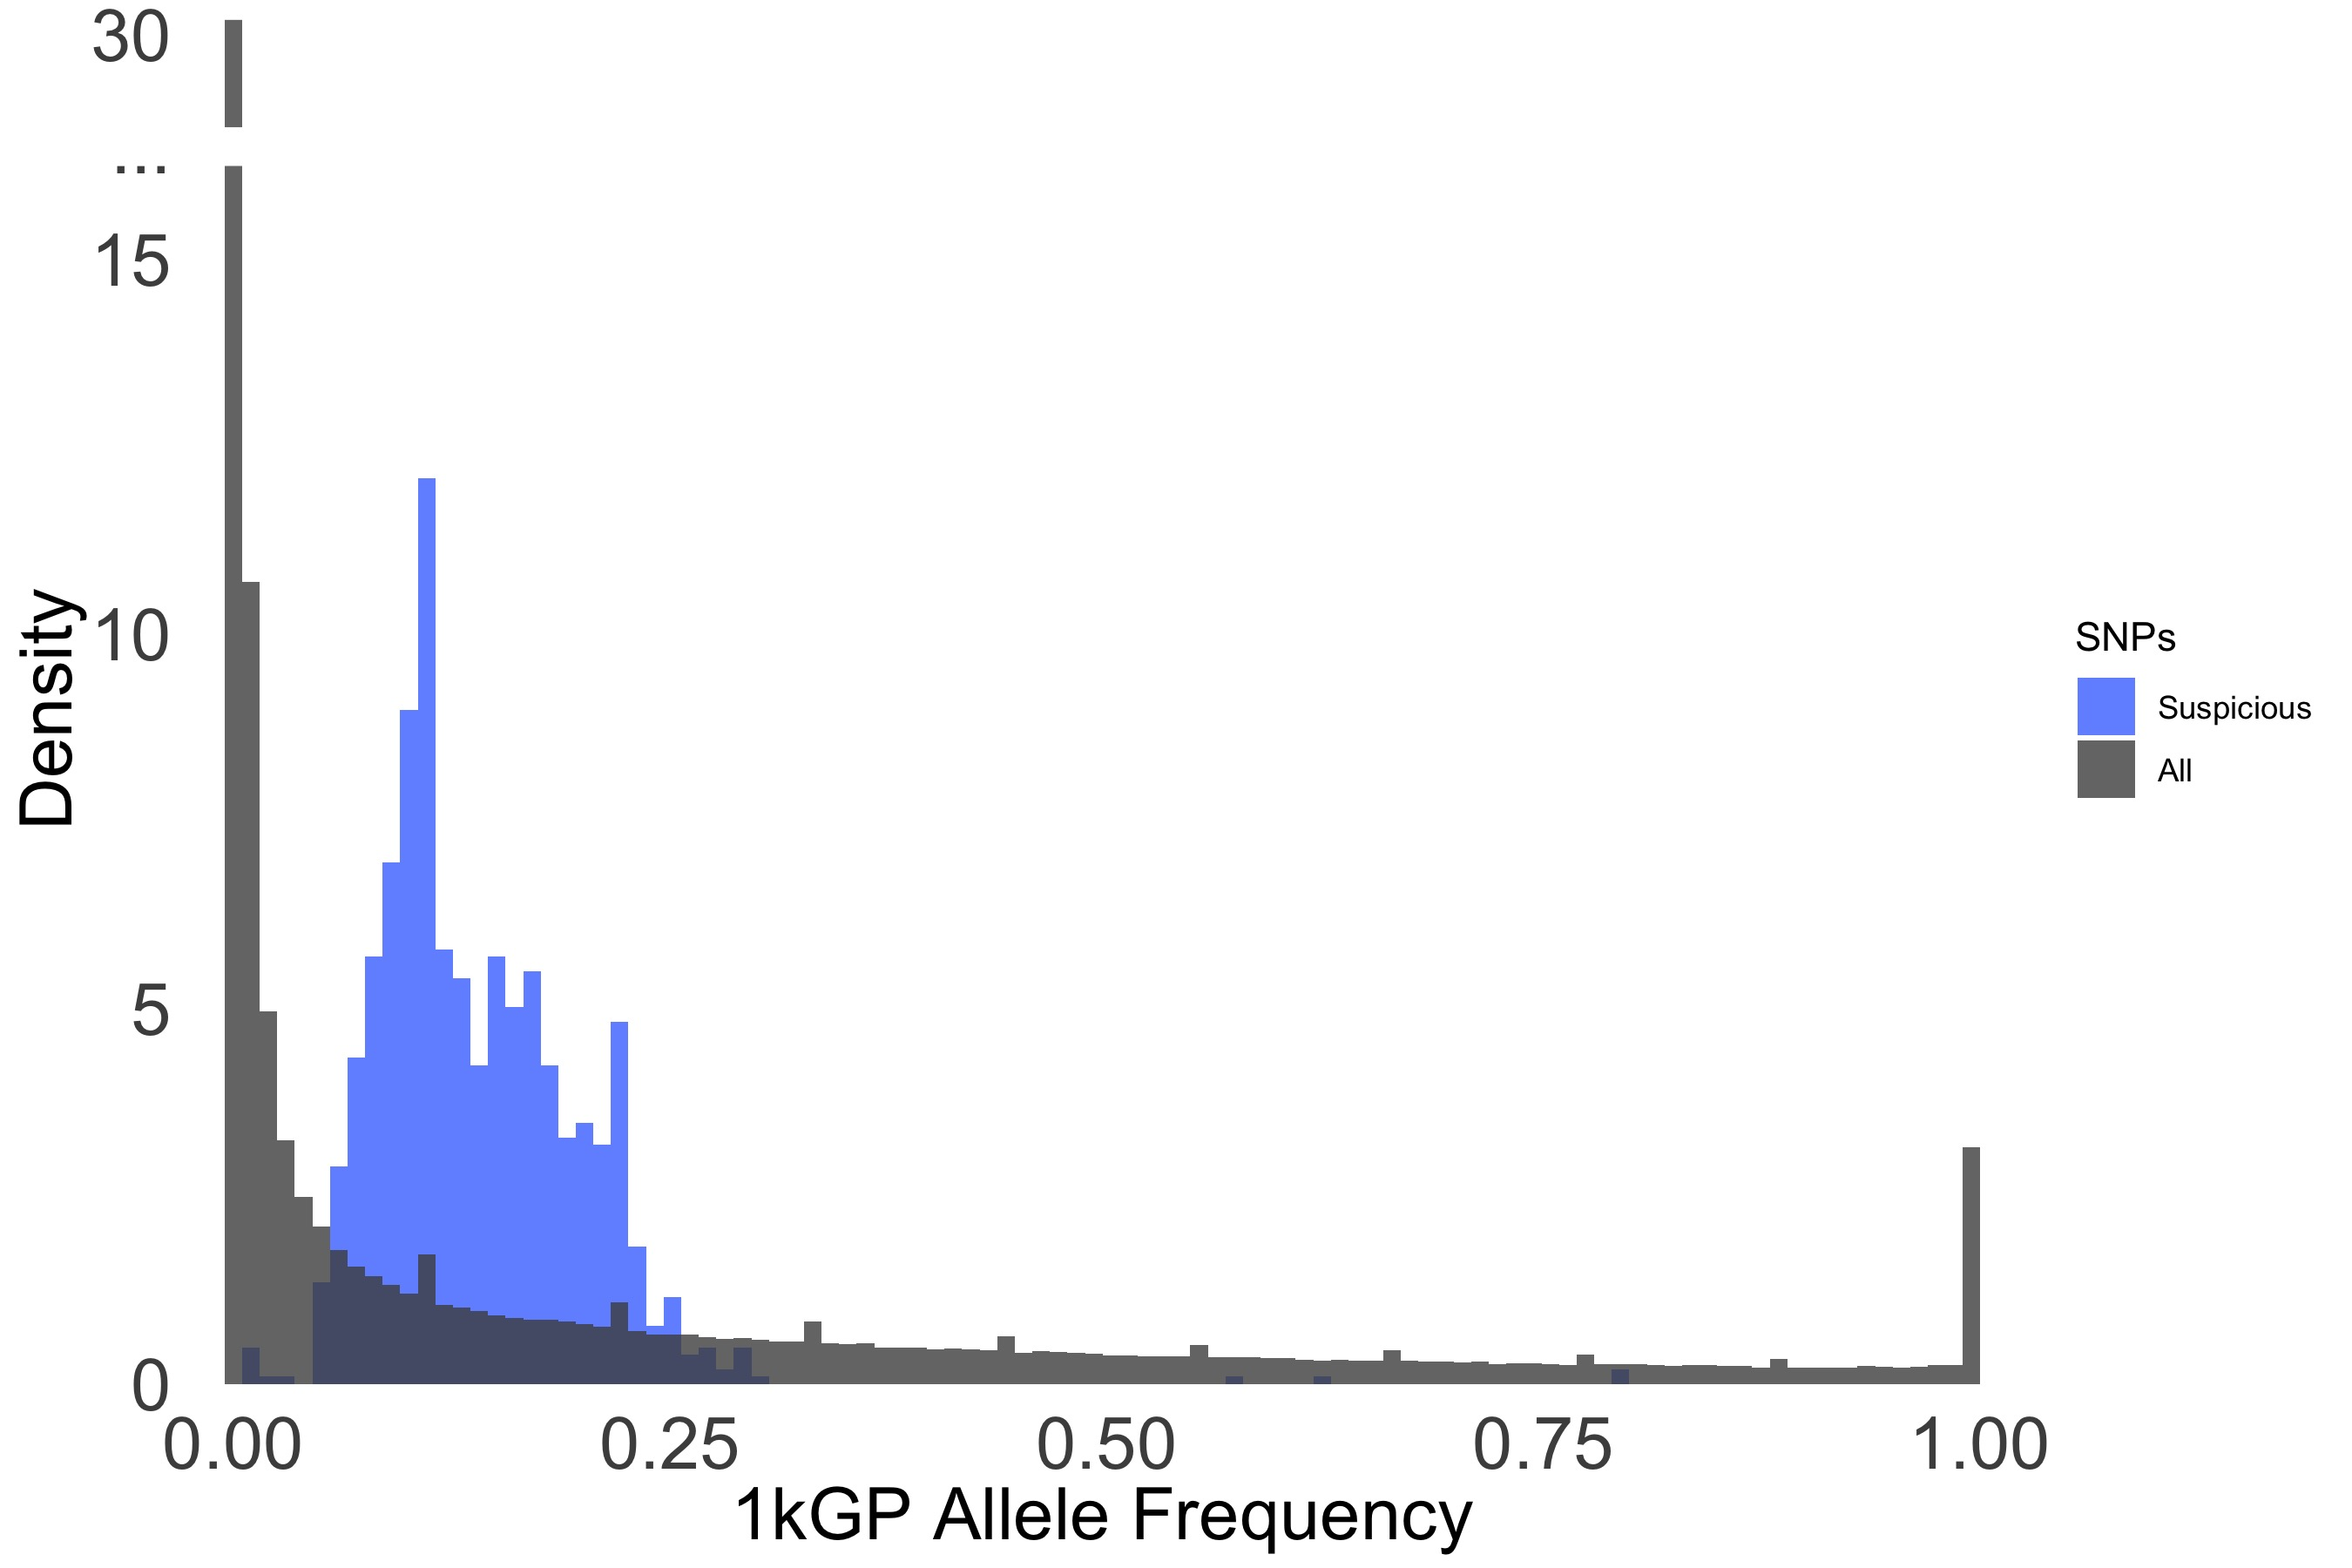
\includegraphics[width=13cm,keepaspectratio]{../Figures/histogram_of_sig_snps.jpg}
\caption{Frequency distribution of the 1034 $Q$ associated SNPs from the single population test in the JPT in blue and all SNPs in black. The association test lacks power to identify variants at low frequencies.}  
\label{histogram_of_sig_snps}
\end{figure}


\begin{figure}
\centering
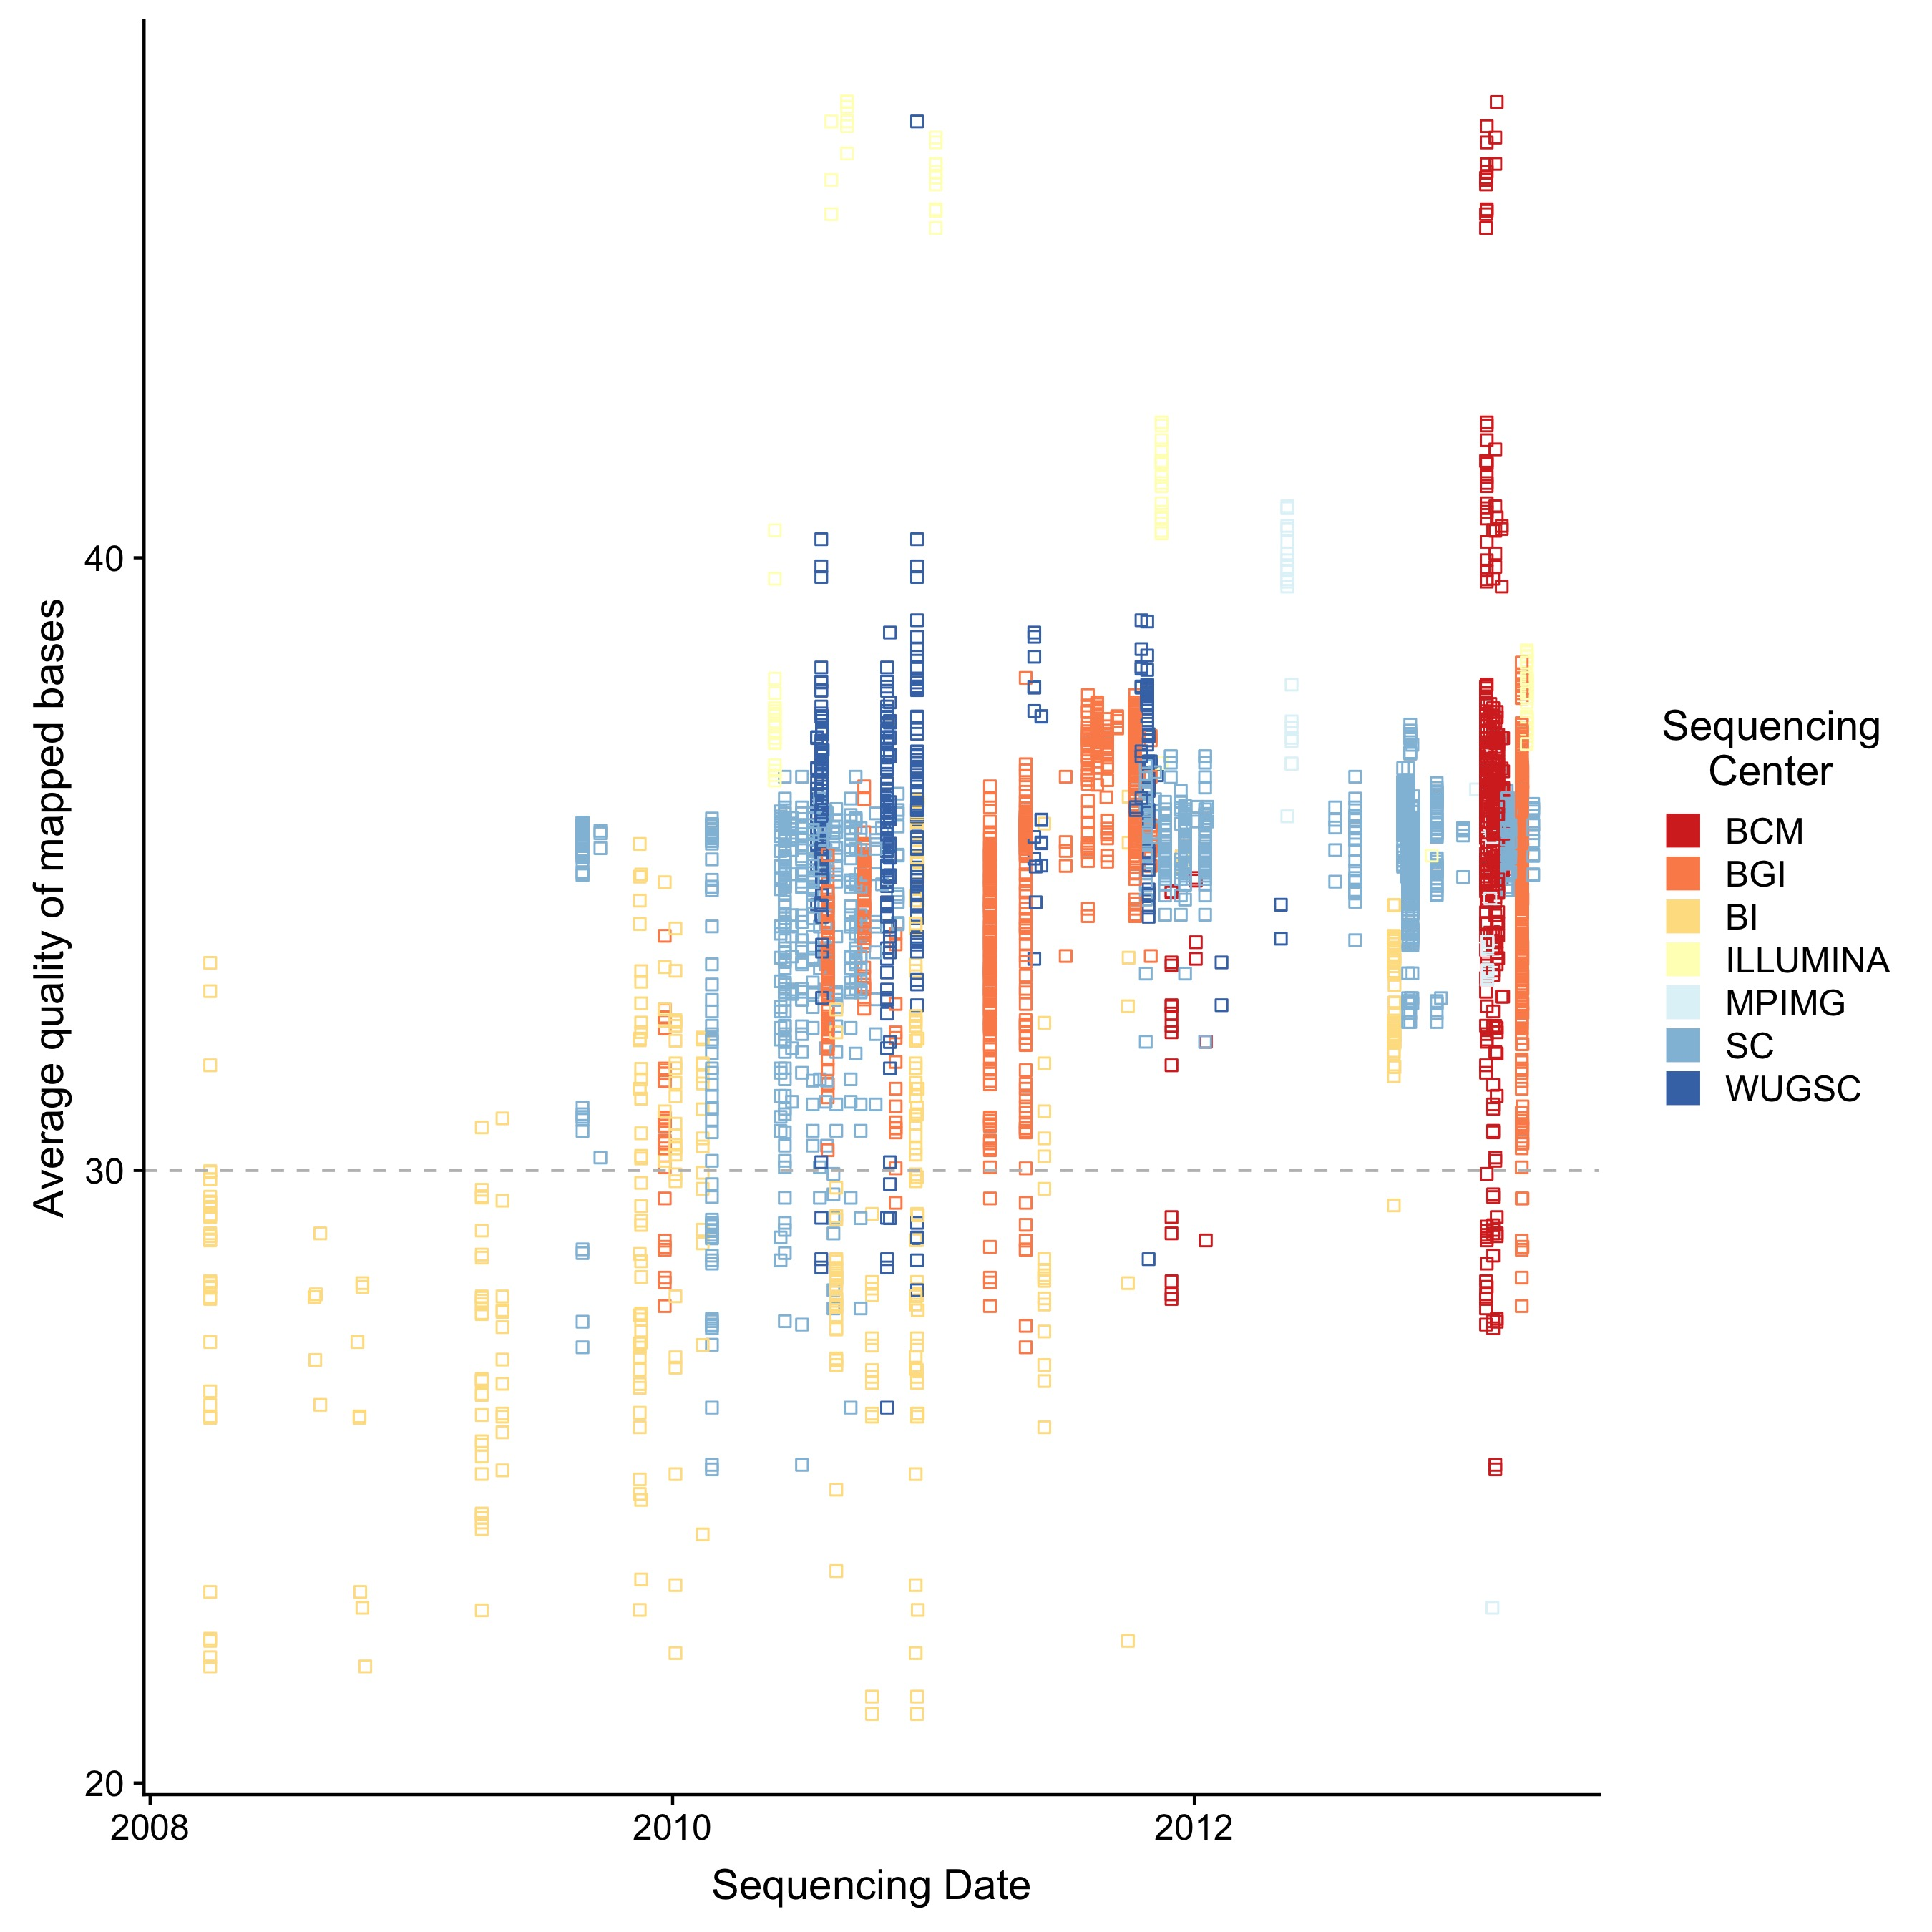
\includegraphics[width=13cm,keepaspectratio]{../Figures/quality_by_center.jpg}
\caption{Sequencing date of samples included in the 1kGP coloured by sequencing centre. Improvements in sequencing platforms coincides with improvement in sequencing quality.}  
\label{quality_by_center}
\end{figure}


\begin{figure}
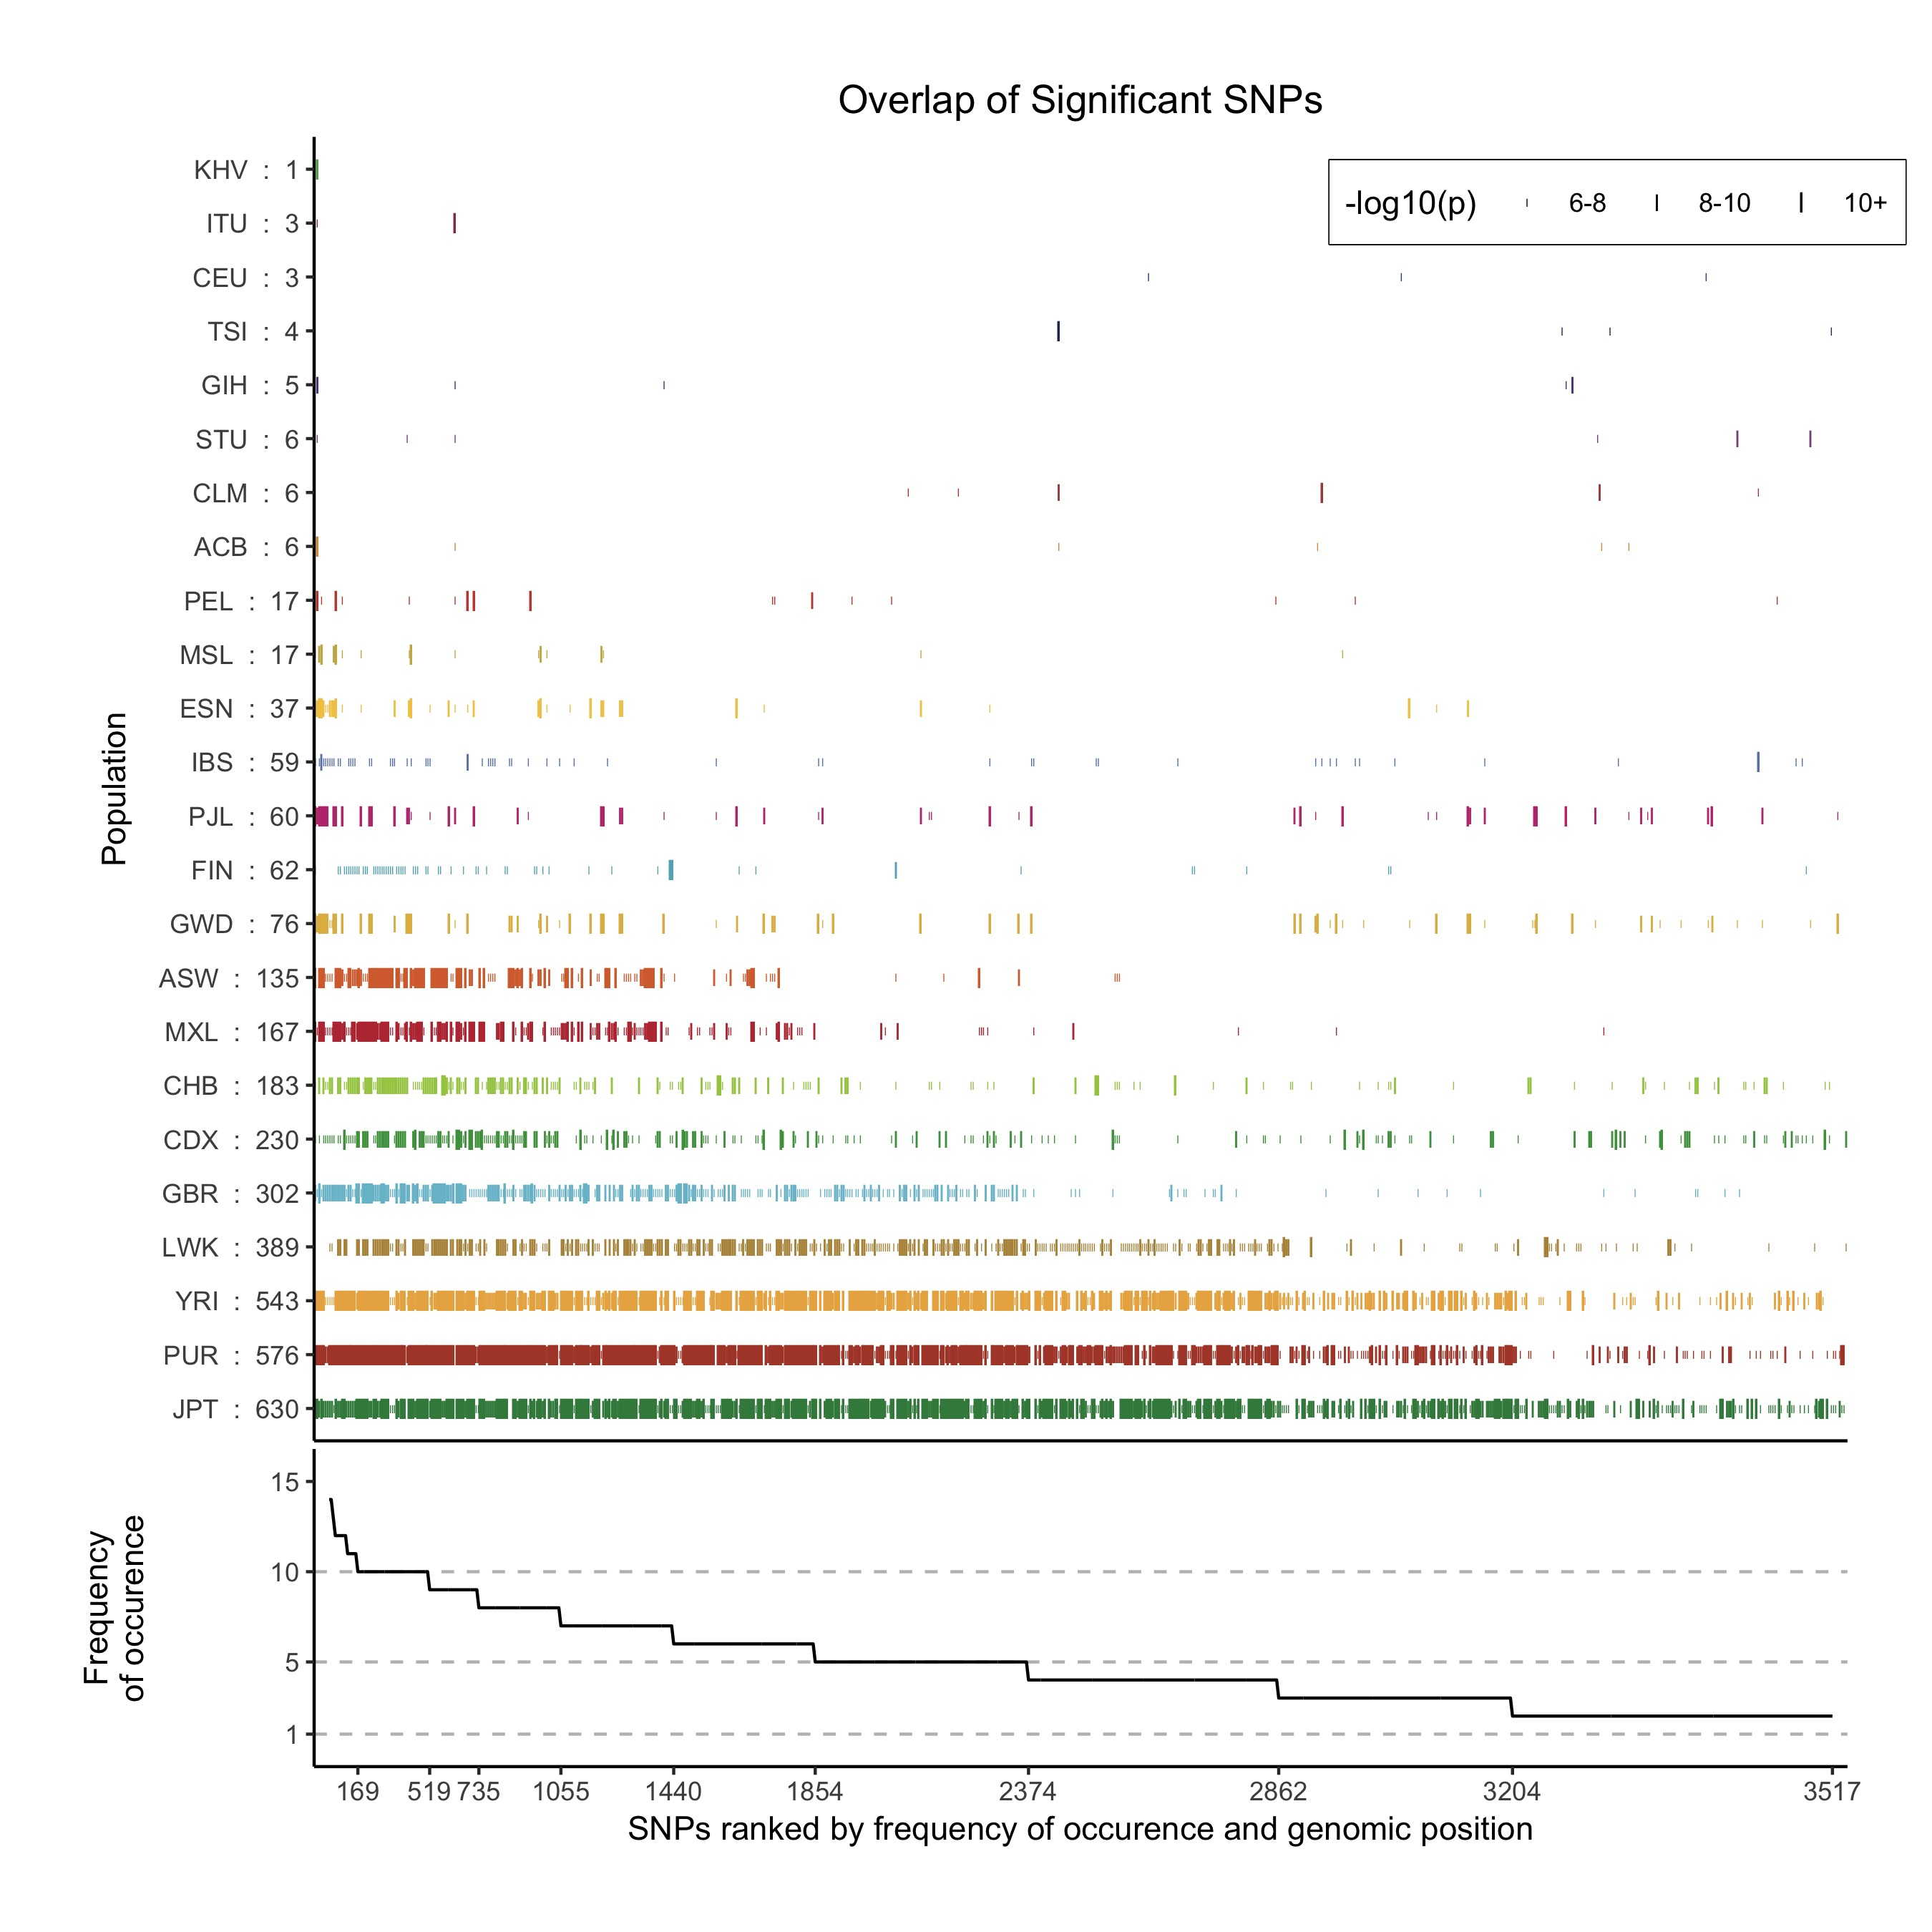
\includegraphics[width=\hsize,keepaspectratio]{../Figures/SNPOverlap6.jpg}

\caption{Variants associated with average quality of mapped bases $Q$ in more than one population.
The size of the vertical bars ( I ) are proportional to the -log10(p) value of that SNP.
The x axis is ranked by the frequency of occurrence of a SNP, then by genomic position.
Phase 1 populations are marked by a star ( * ).
The line plot underneath shows the number of populations for which a variant has reached significance.
The populations that tend to have the most individuals with low $Q$ also tend to have the most variants associated to $Q$.}
  \label{OverLap}
\end{figure}

\begin{figure}[ht]
\centering
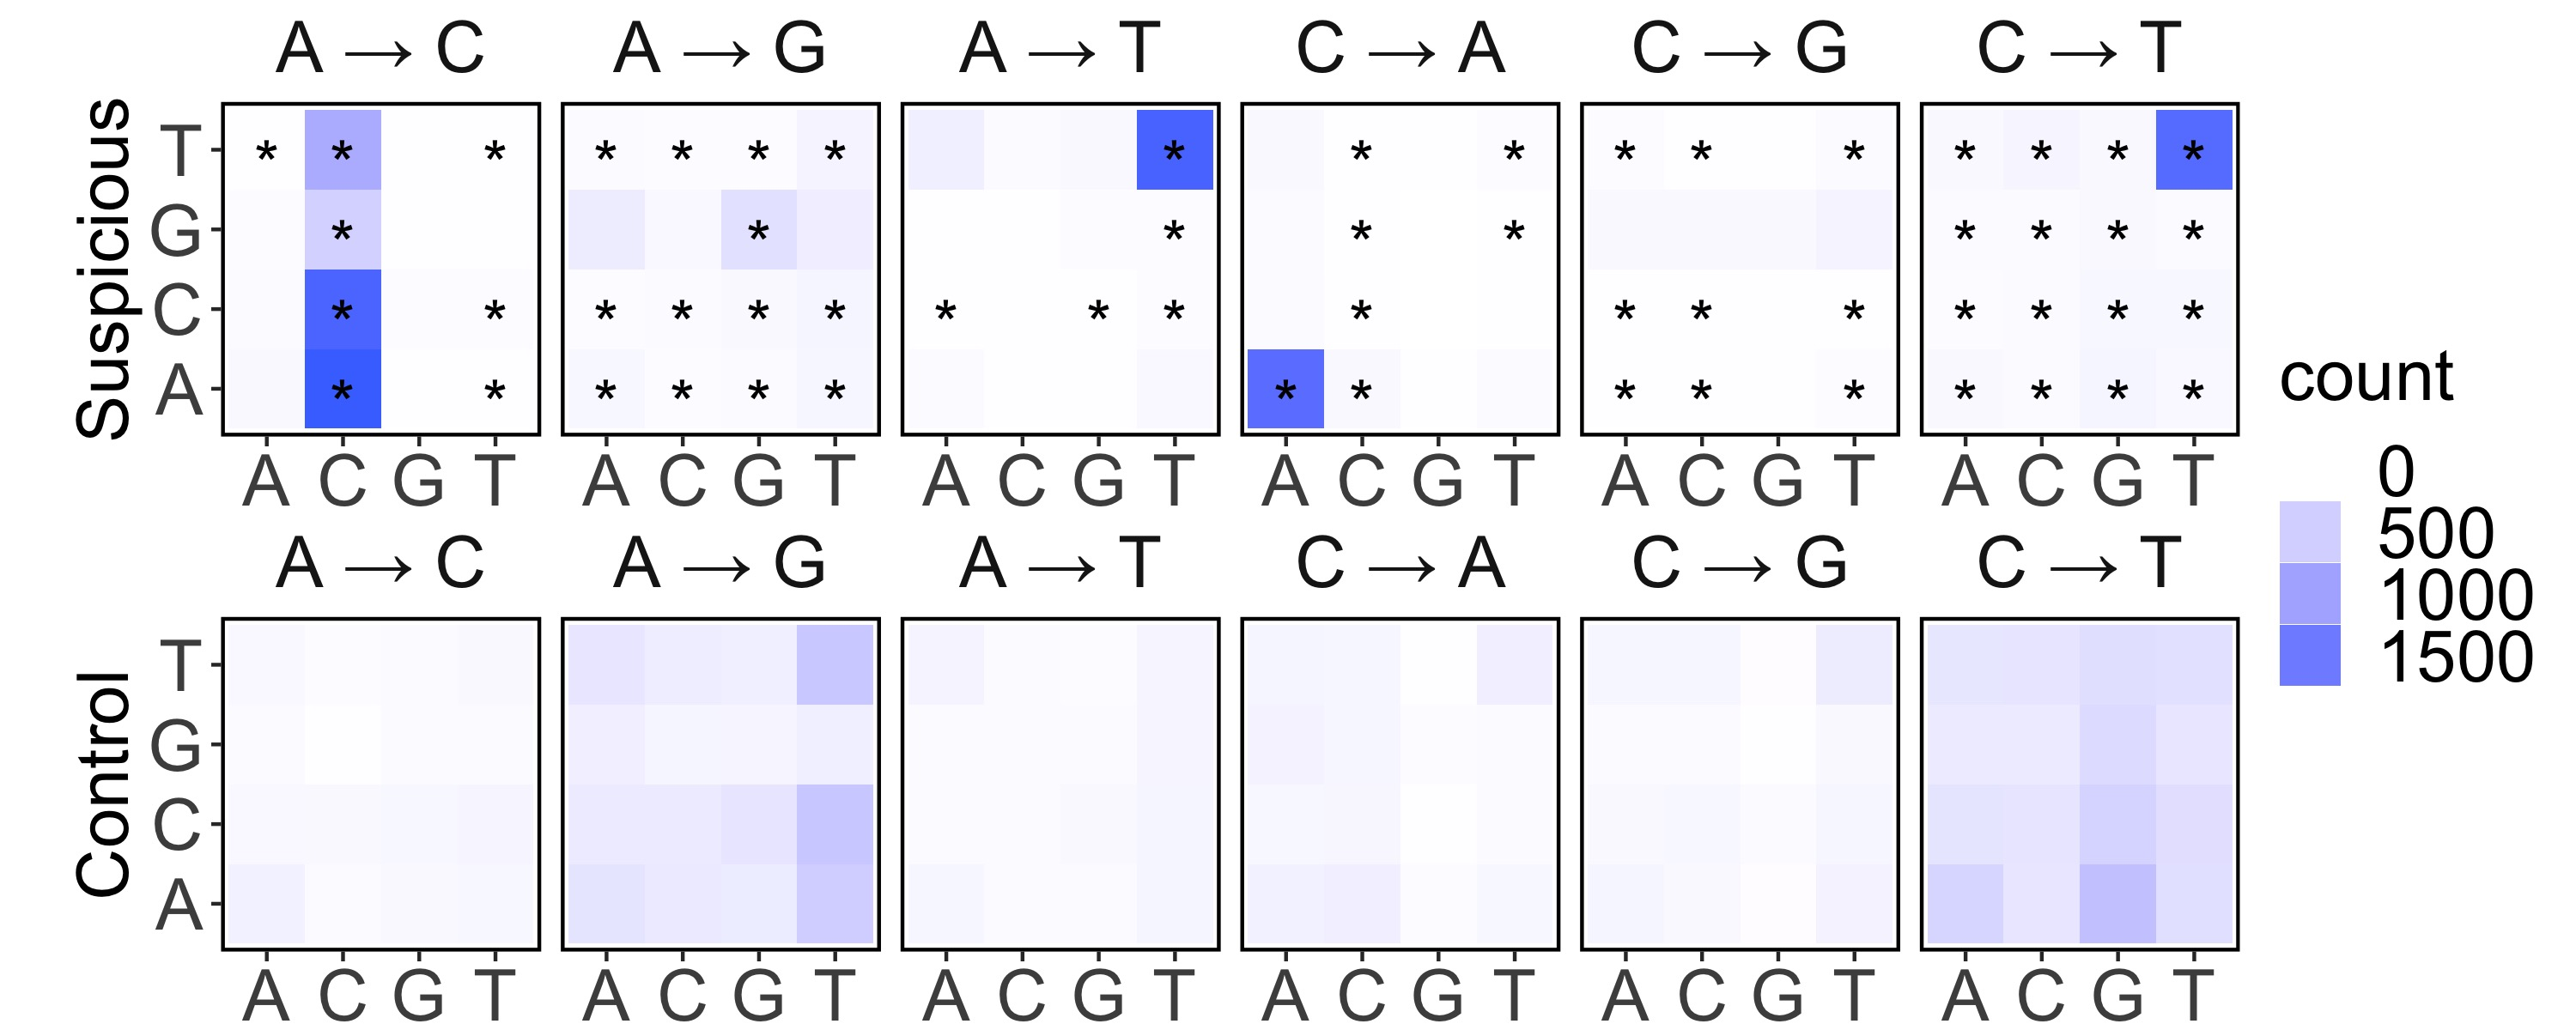
\includegraphics[width=13cm,keepaspectratio]{../Figures/strict_gcat_mutational_enrichment.jpg}
\caption{Mutation spectrum of the 15,270 $Q$-associated variants that pass the 1kGP strict mask filter, compared to a random set of non-associated variants. A large fraction of the  $Q$-associated variants have the *AC${\rightarrow}$*CC mutational pattern. There is also an enrichment in TAT${\rightarrow}$TTT, TCT${\rightarrow}$TTT and ACA${\rightarrow}$AAA (reverse complement : TGT${\rightarrow}$TTT). These three enrichments can be summarized as T*T${\rightarrow}$TTT. Stars ( * ) indicate significant difference from the mutational spectrum of a set of control variants of equal size.}  
\label{strict_gcat_mutational_enrichment}
\end{figure}


\begin{figure}[ht]
\centering
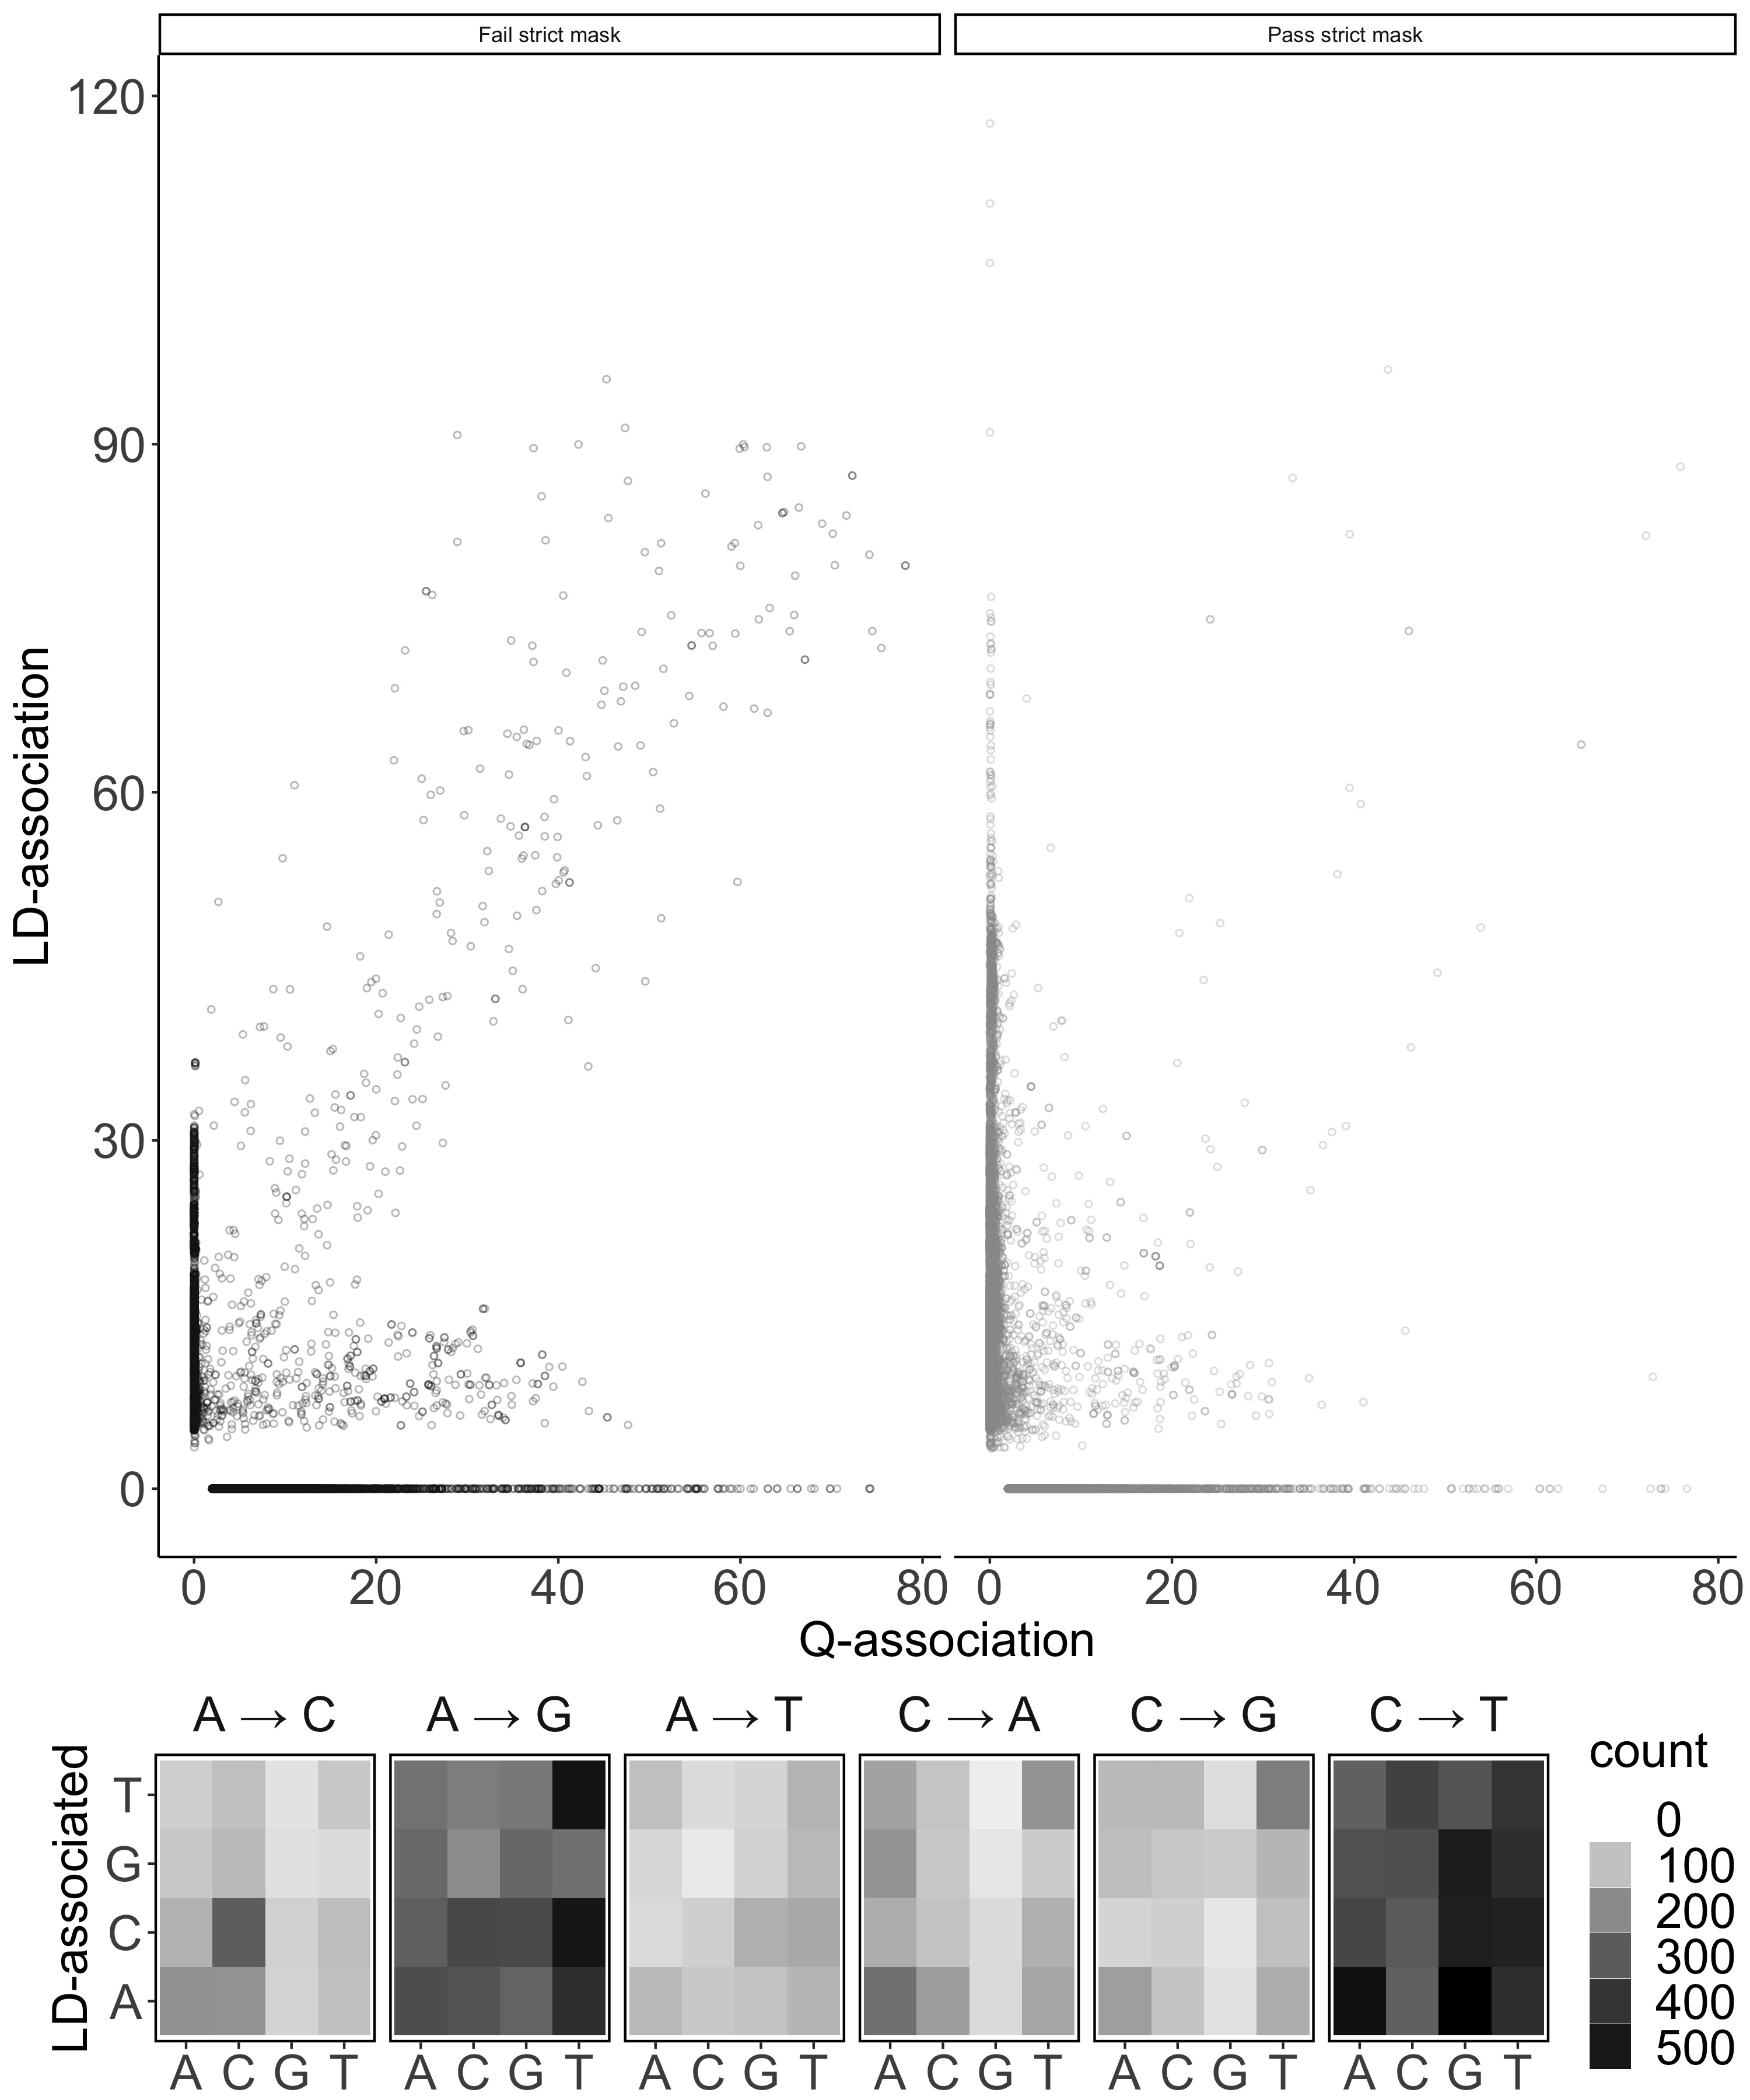
\includegraphics[width=13cm,keepaspectratio]{../Figures/Mafessoni_MutSpect.jpg}
\caption{ \textbf{A} Comparison of the p-values from the association to unusual LD from \cite{mafessoni2018turning} and the p-values from the GCAT association test to quality metrics.
\textbf{B} Mutation spectrum of the variants significantly associated to unusual LD from \cite{mafessoni2018turning}. }  
\label{Mafessoni_MutSpect}
\end{figure}

\begin{figure}[ht]
\centering
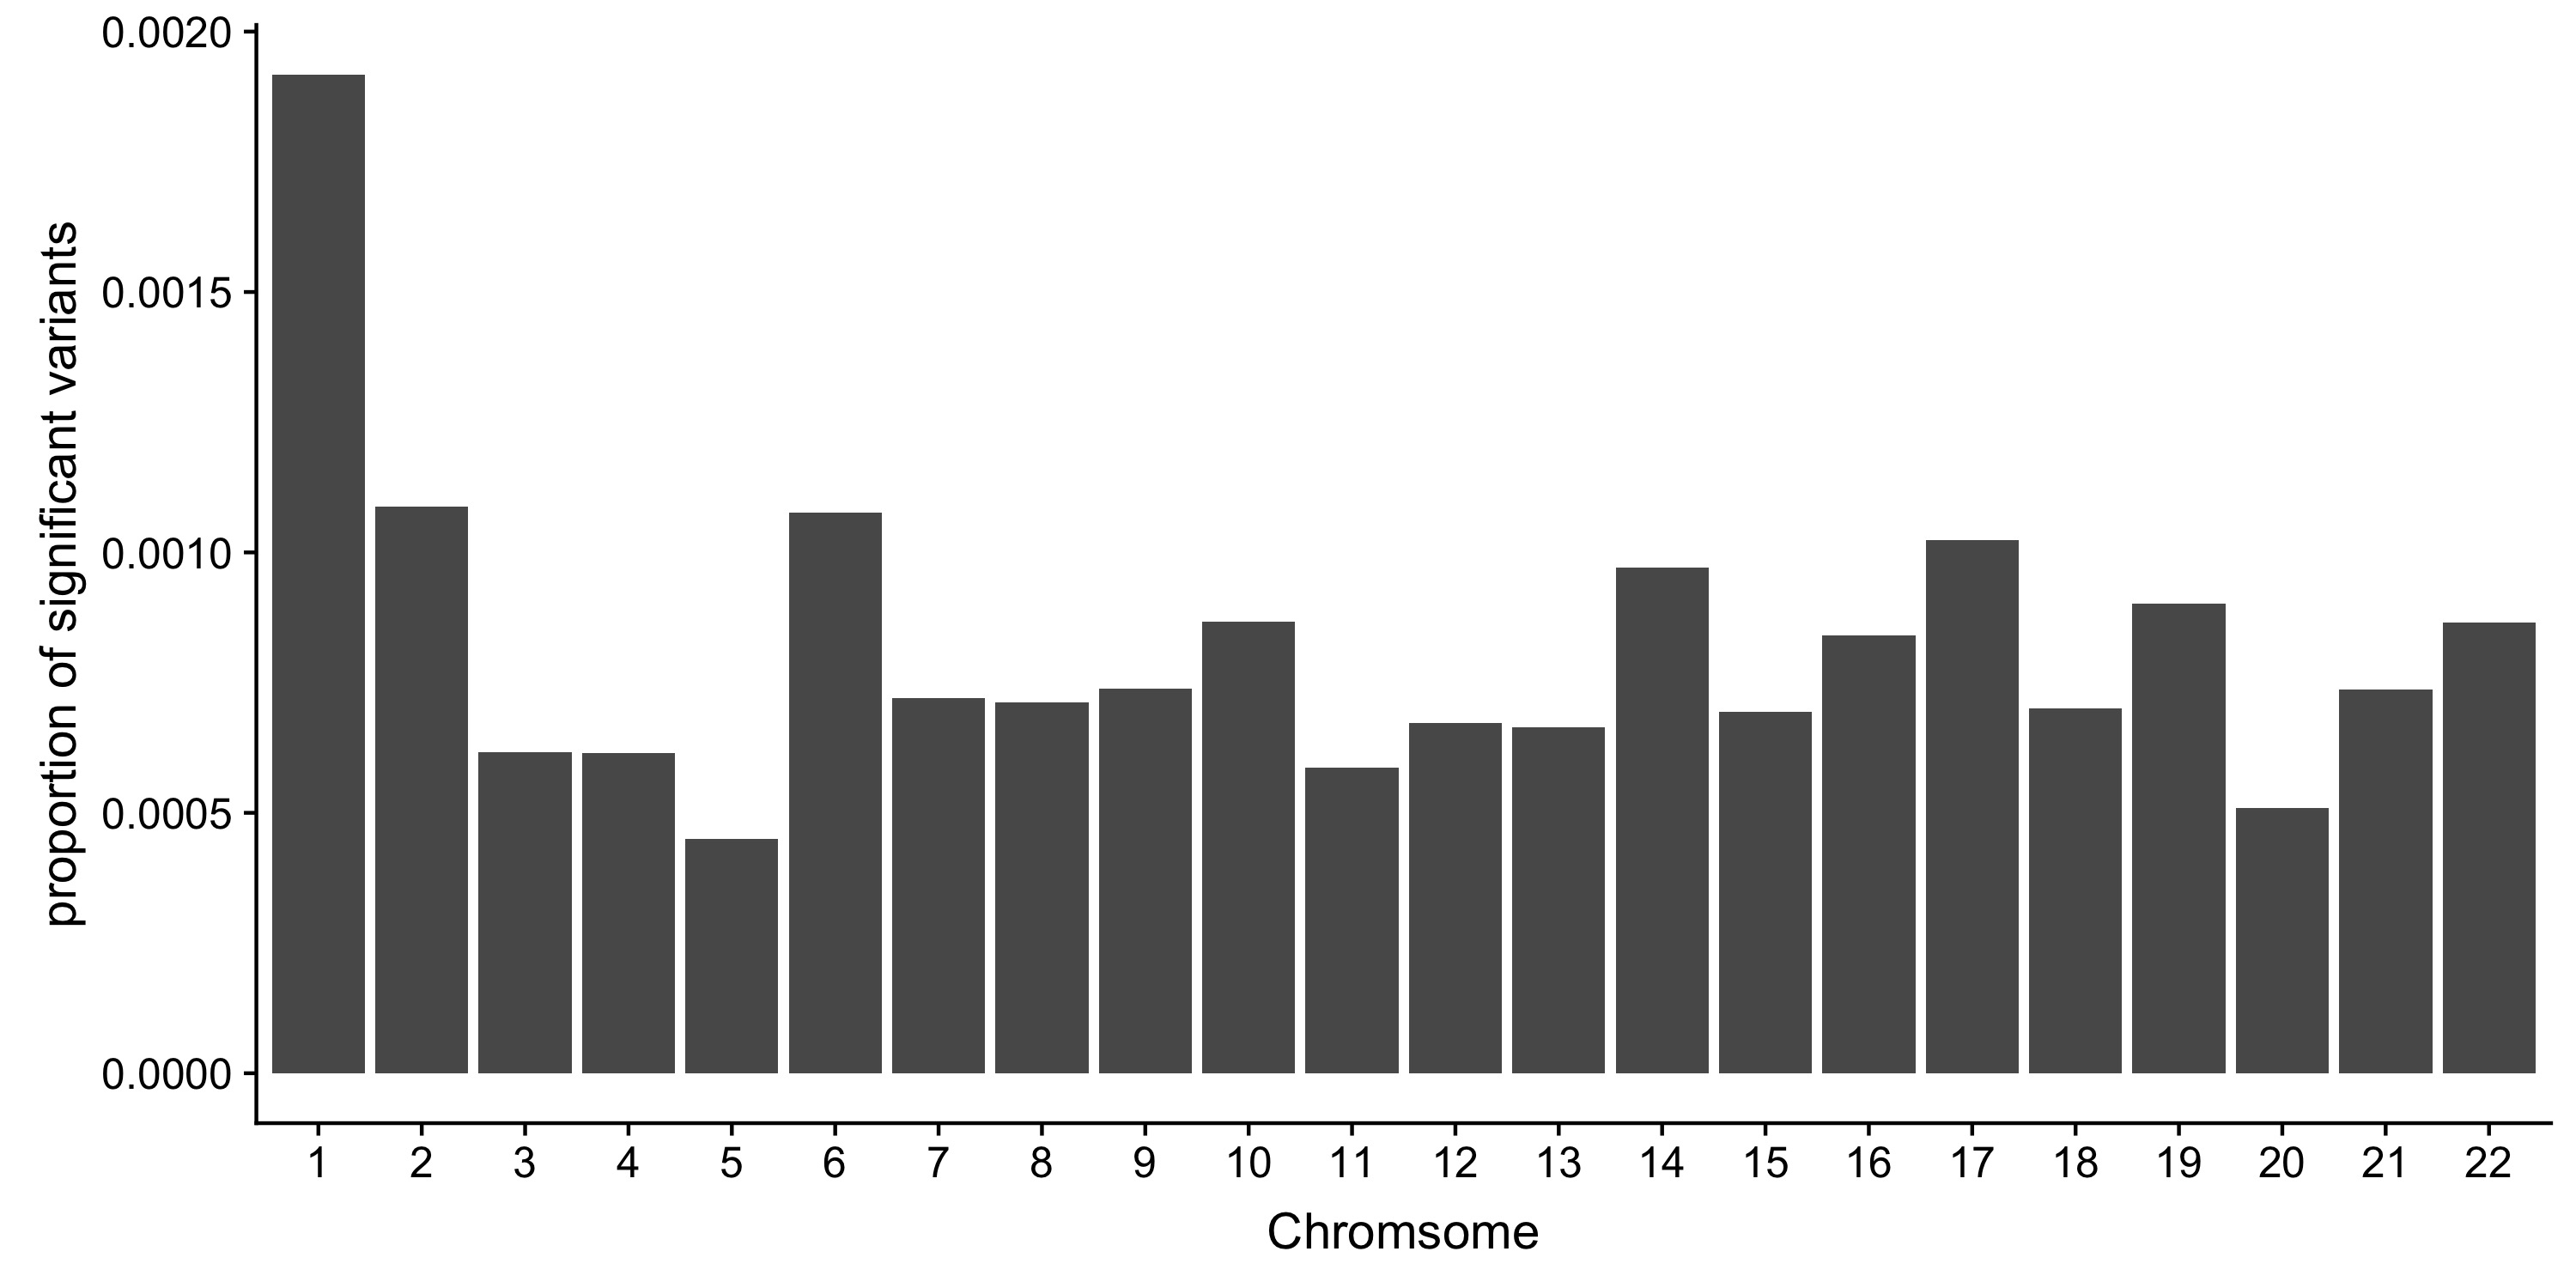
\includegraphics[width=11cm,keepaspectratio]{../Figures/CountPerChrom.jpg}
\caption{The proportion of $Q$-associated variants per chromosome.}  
\label{CountPerChrom}
\end{figure}

\begin{figure}[ht]
\centering
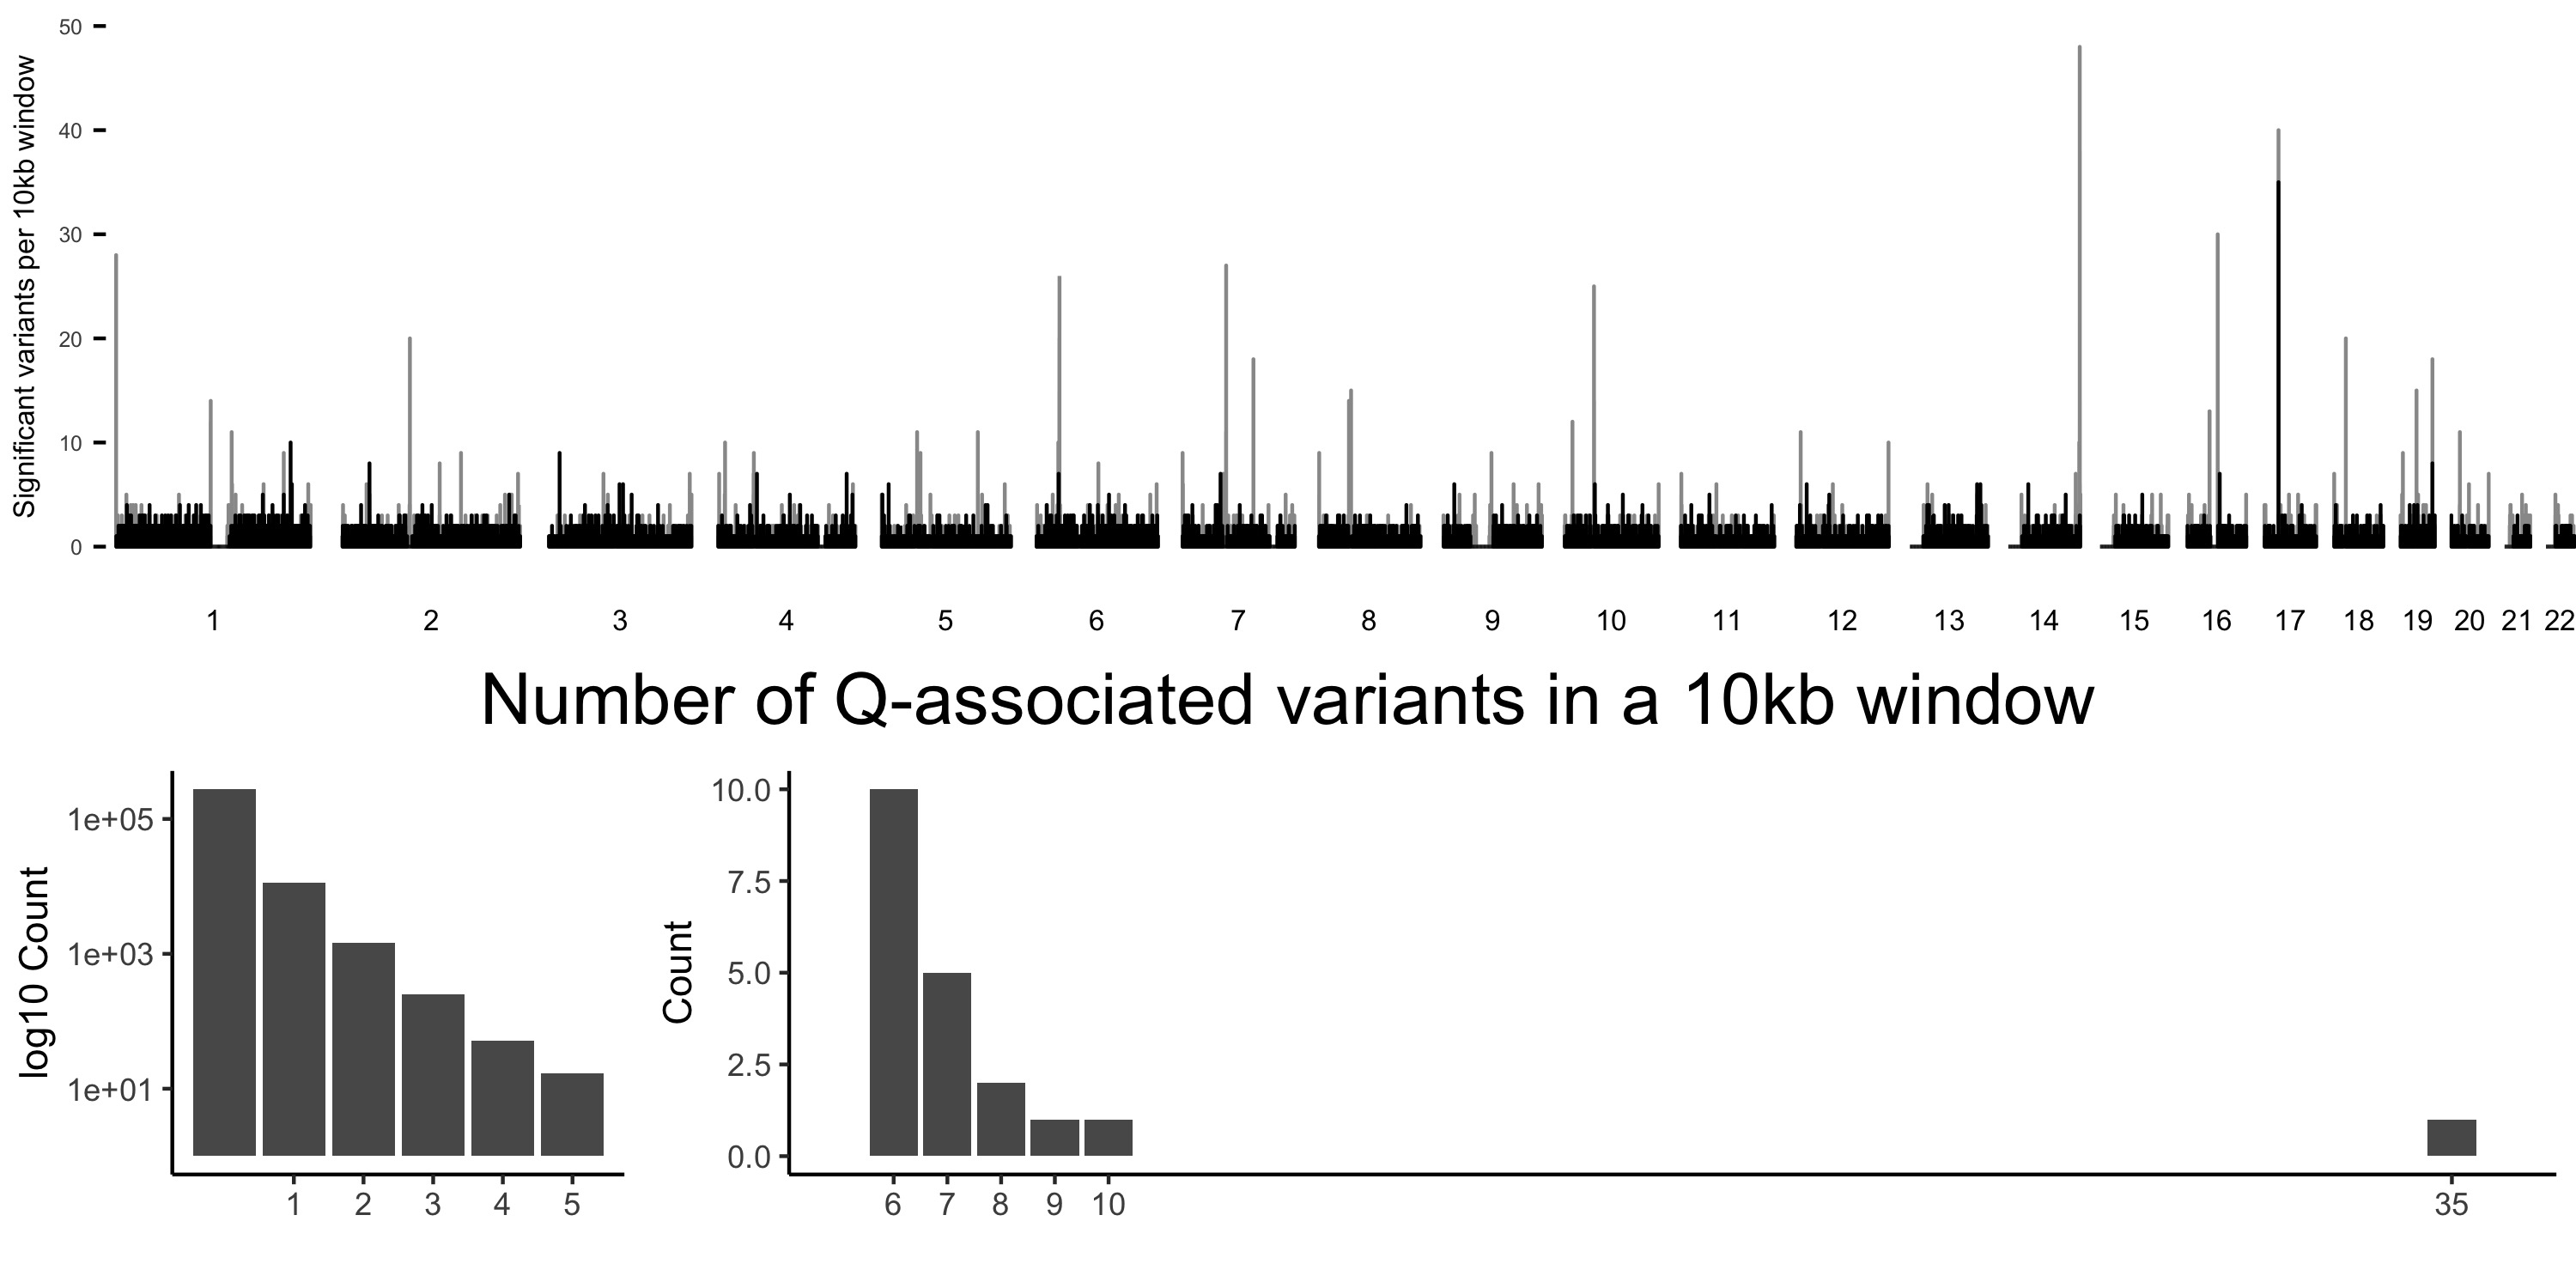
\includegraphics[width=15cm,keepaspectratio]{../Figures/VariantDensity.jpg}
\caption{The number of $Q$-associated variants per 10kb window across the genome.
Grey bars indicate regions within and black bars indicate regions outside the 1000 Genomes Project strict mask.
One region not flagged by the 1000 Genomes Project strict mask in chromosome 17 has more than 10 variants per window.}  
\label{VariantDensity}
\end{figure}

\begin{figure}[ht]
\centering
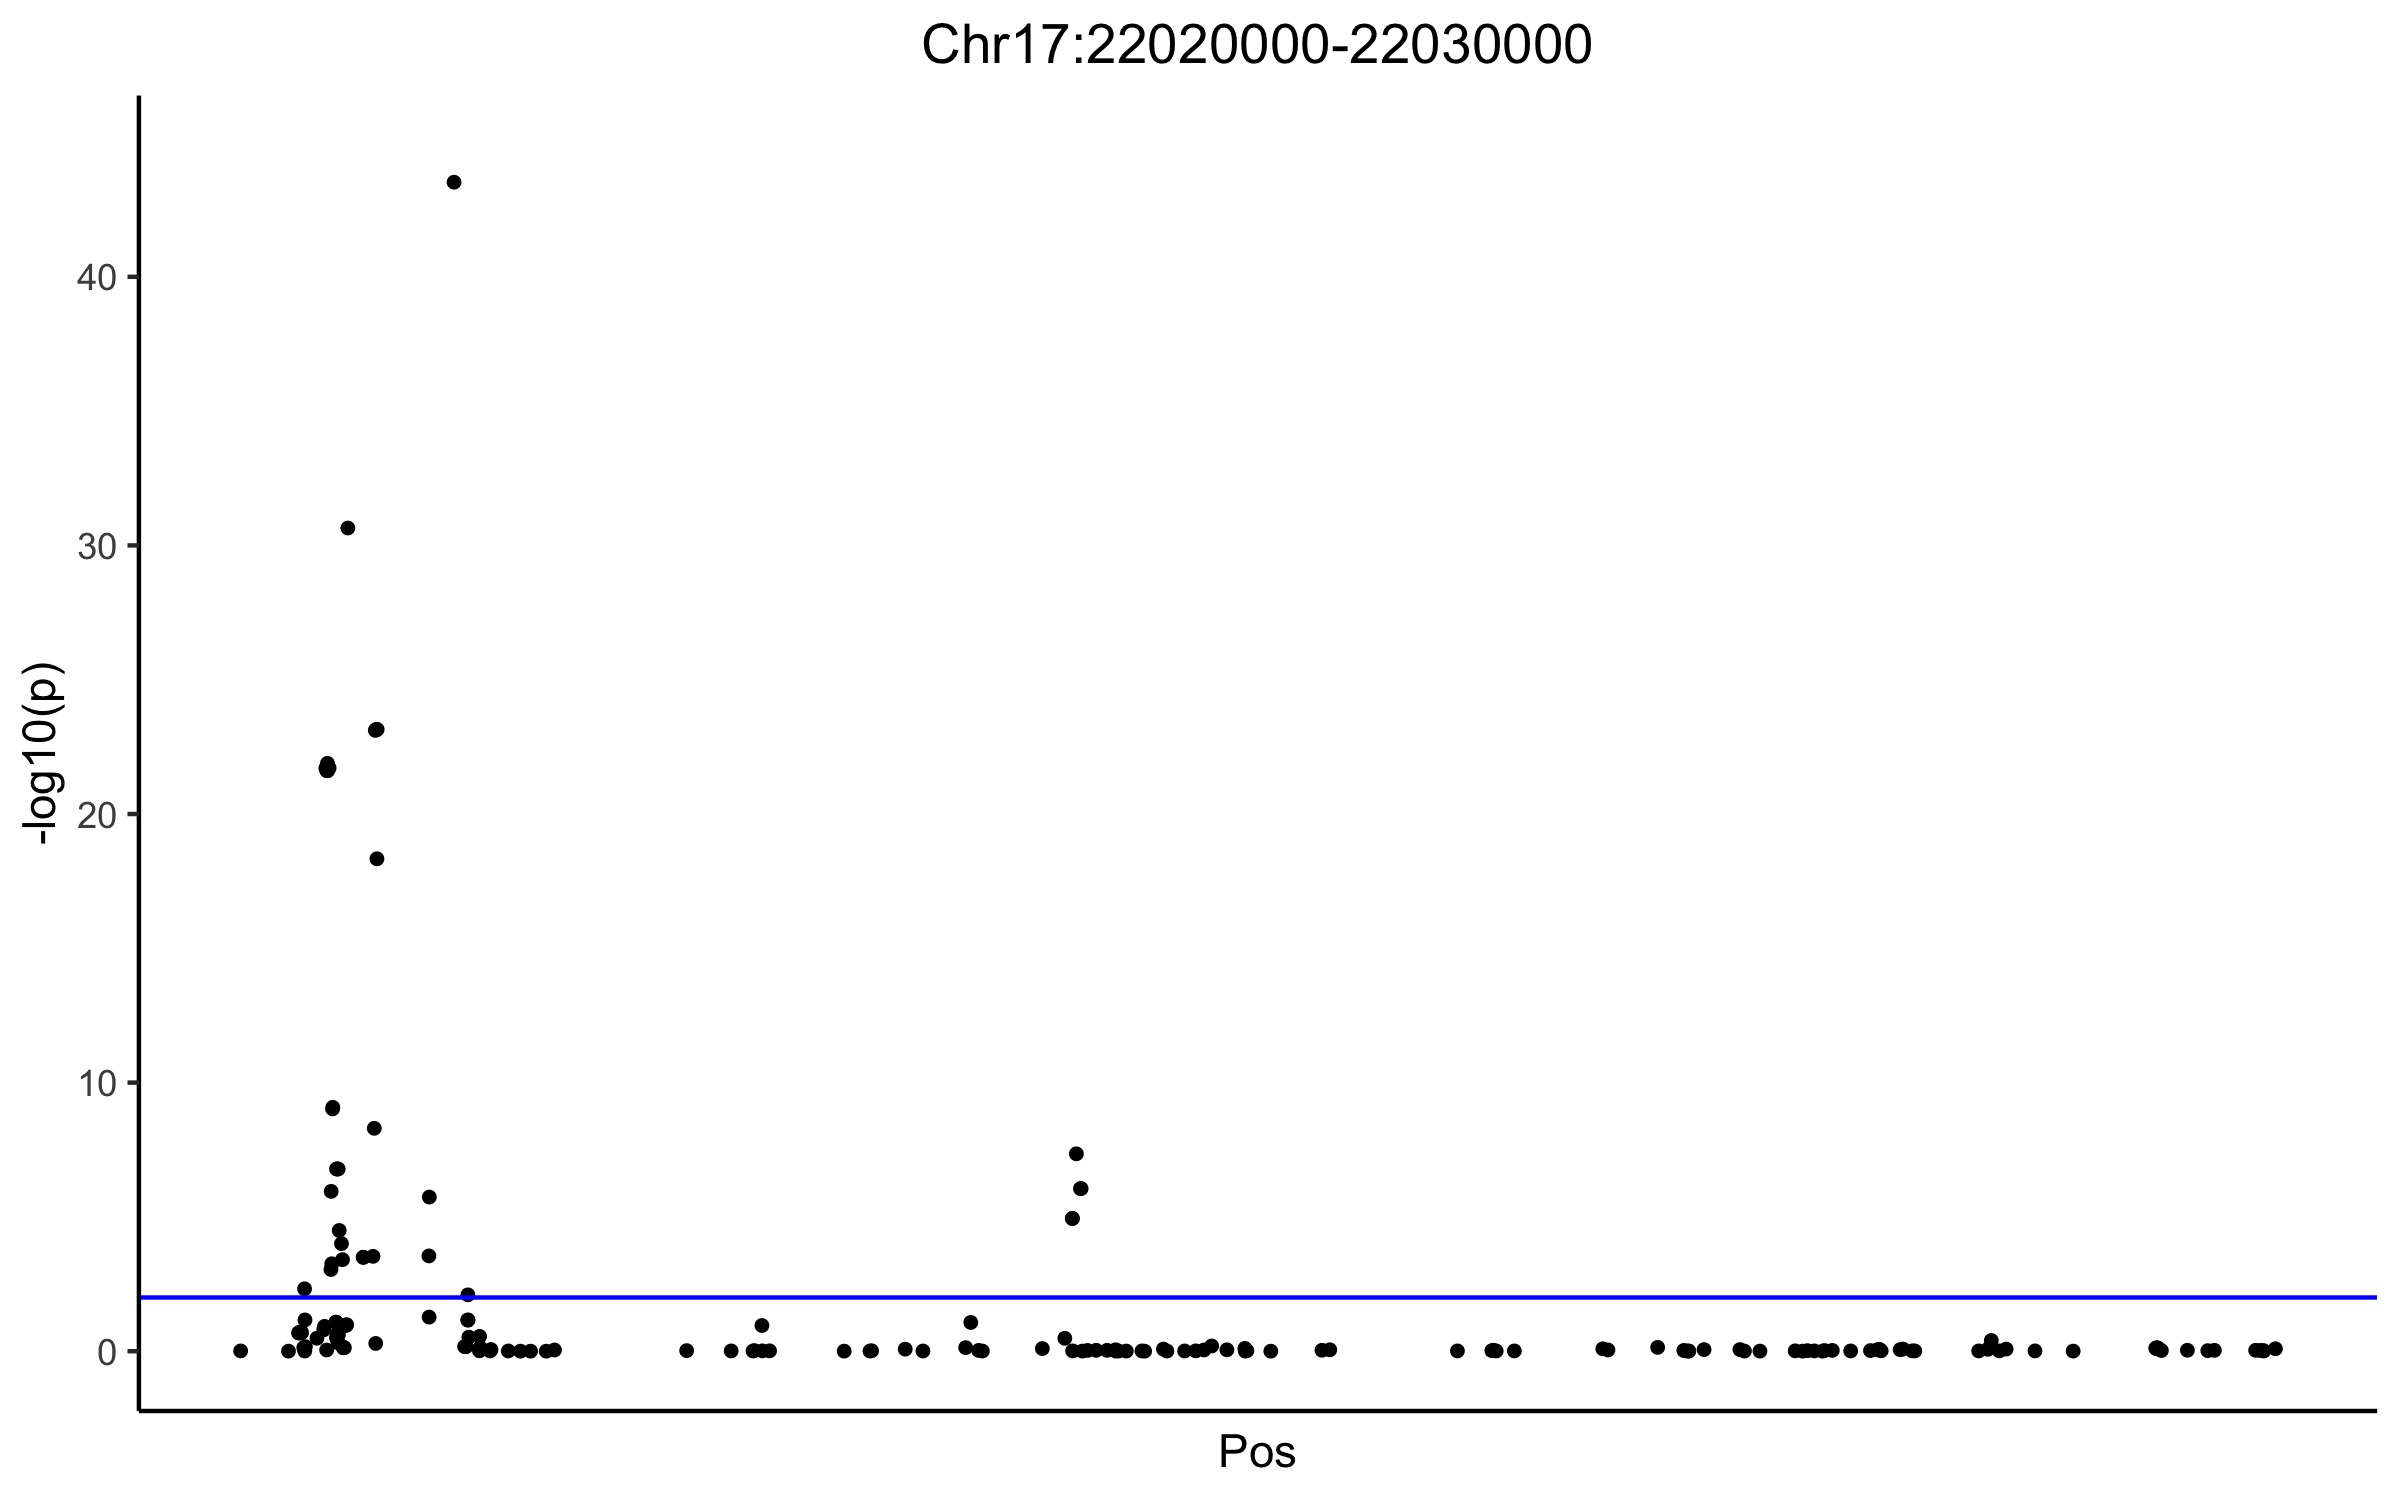
\includegraphics[width=10cm,keepaspectratio]{../Figures/RegionOver10.jpg}
\caption{Manhattan plot of the $-\log_{10}(p)$ values for the reverse GWAS logistic regression analysis for the 10kb window with the most  $Q$-associated variants per 10kb across the genome.}  
\label{Top10}
\end{figure}

\begin{figure}[ht]
\centering
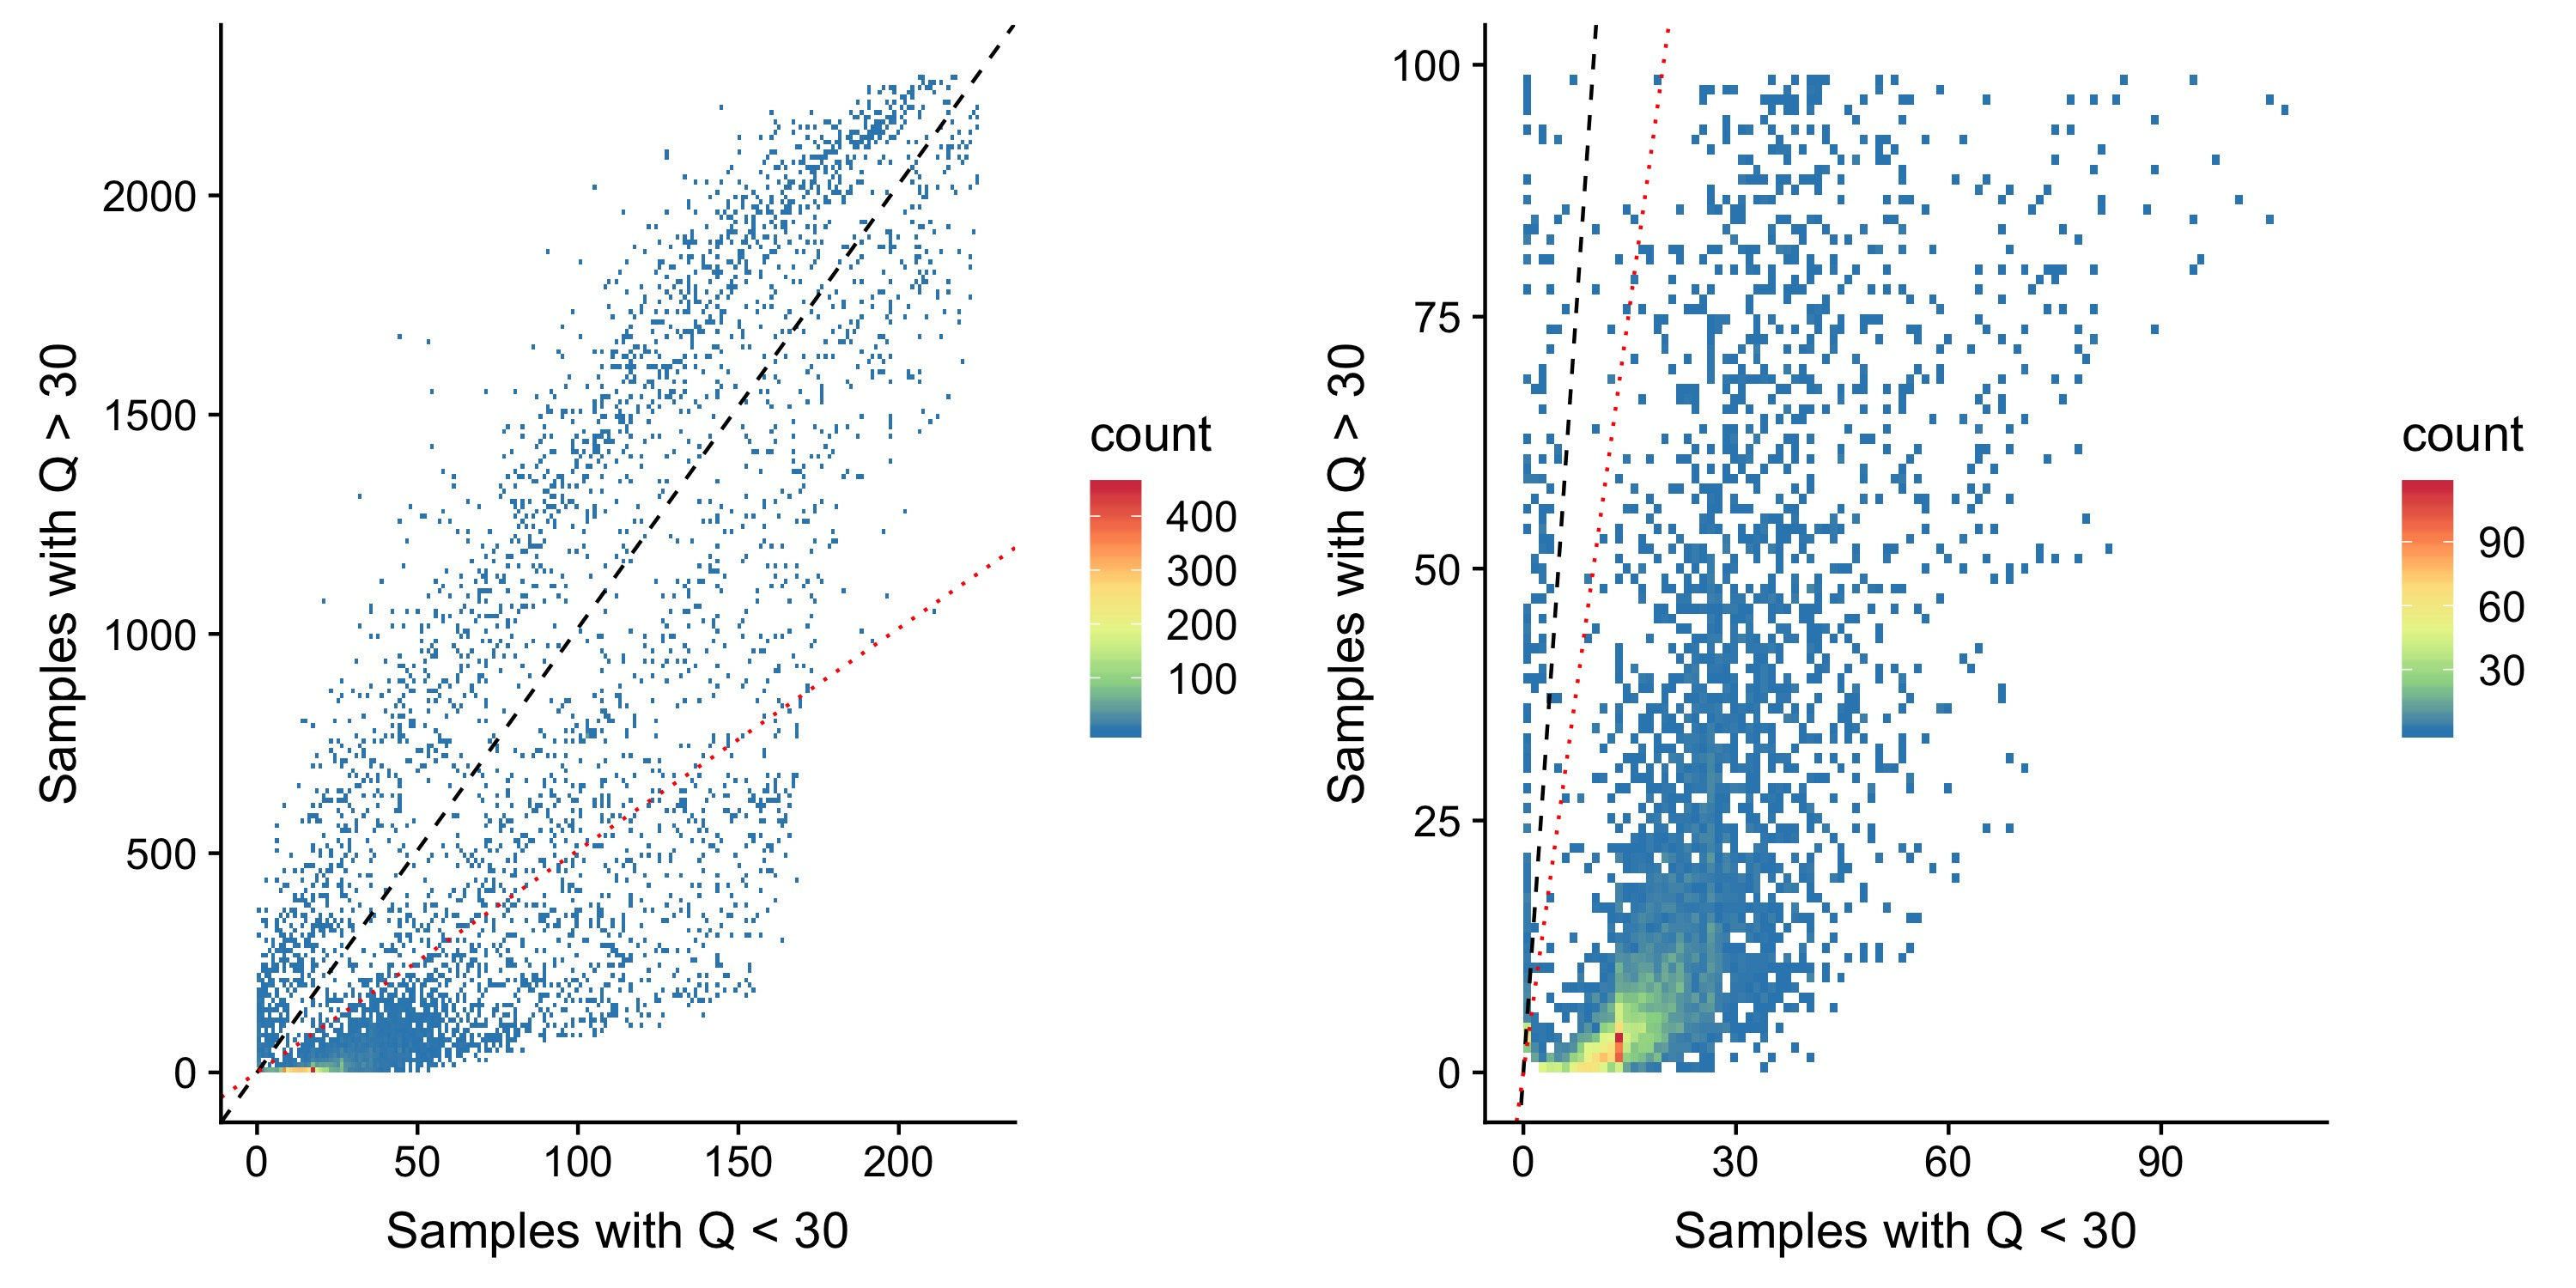
\includegraphics[width=15cm,keepaspectratio]{../Figures/OverUnder30.jpg}
\caption{Site frequency spectrum plot comparing the allele frequency difference between individuals with low- and high-$Q$. The black dashed lines indicates equal allele frequencies while the red dotted line for variants twice as frequent in individuals with $Q$ scores below 30. Two clusters of are visible, where the majority (92.7\%) of the $Q$-associated variants are more than twice as frequent in individuals with low-$Q$.}  
\label{90HanSFS_full}
\end{figure}

\begin{figure}[ht]
\centering
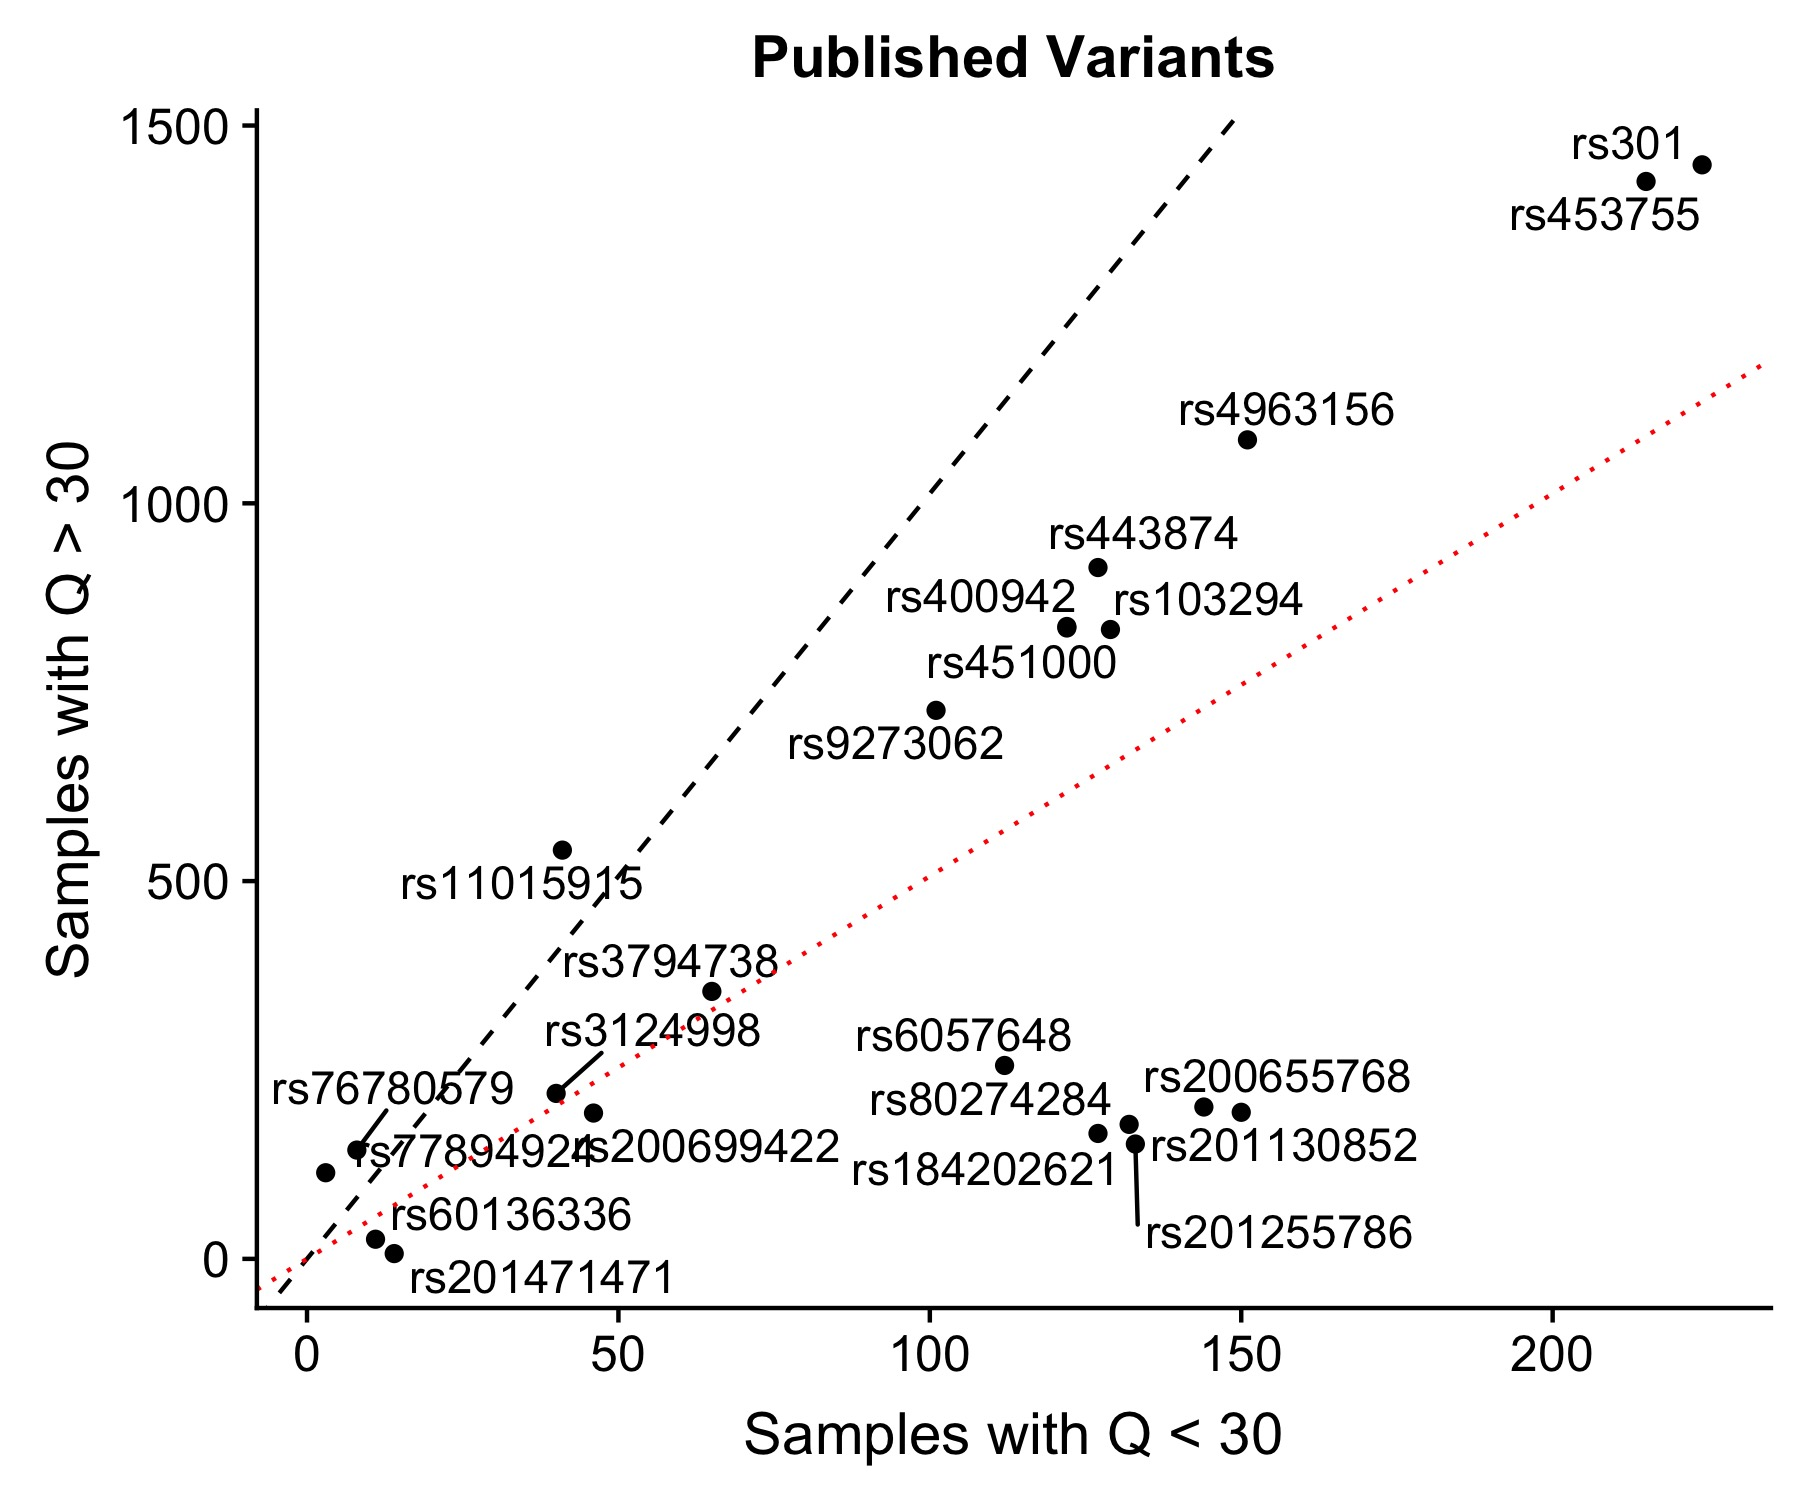
\includegraphics[width=15cm,keepaspectratio]{../Figures/Published_OverUnder30.jpg}
\caption{Site frequency spectrum plot comparing the frequency of $Q$-associated variants identified in publications, for individuals with $Q$ scores above and below 30. The black dashed lines indicates equal allele frequencies while the red dotted line for variants twice as frequent in individuals with $Q$ scores below 30. Each of the rsIDs of the variants are labelled for clarity.}  
\label{Pub_30}
\end{figure}

\begin{figure}[ht]
\centering
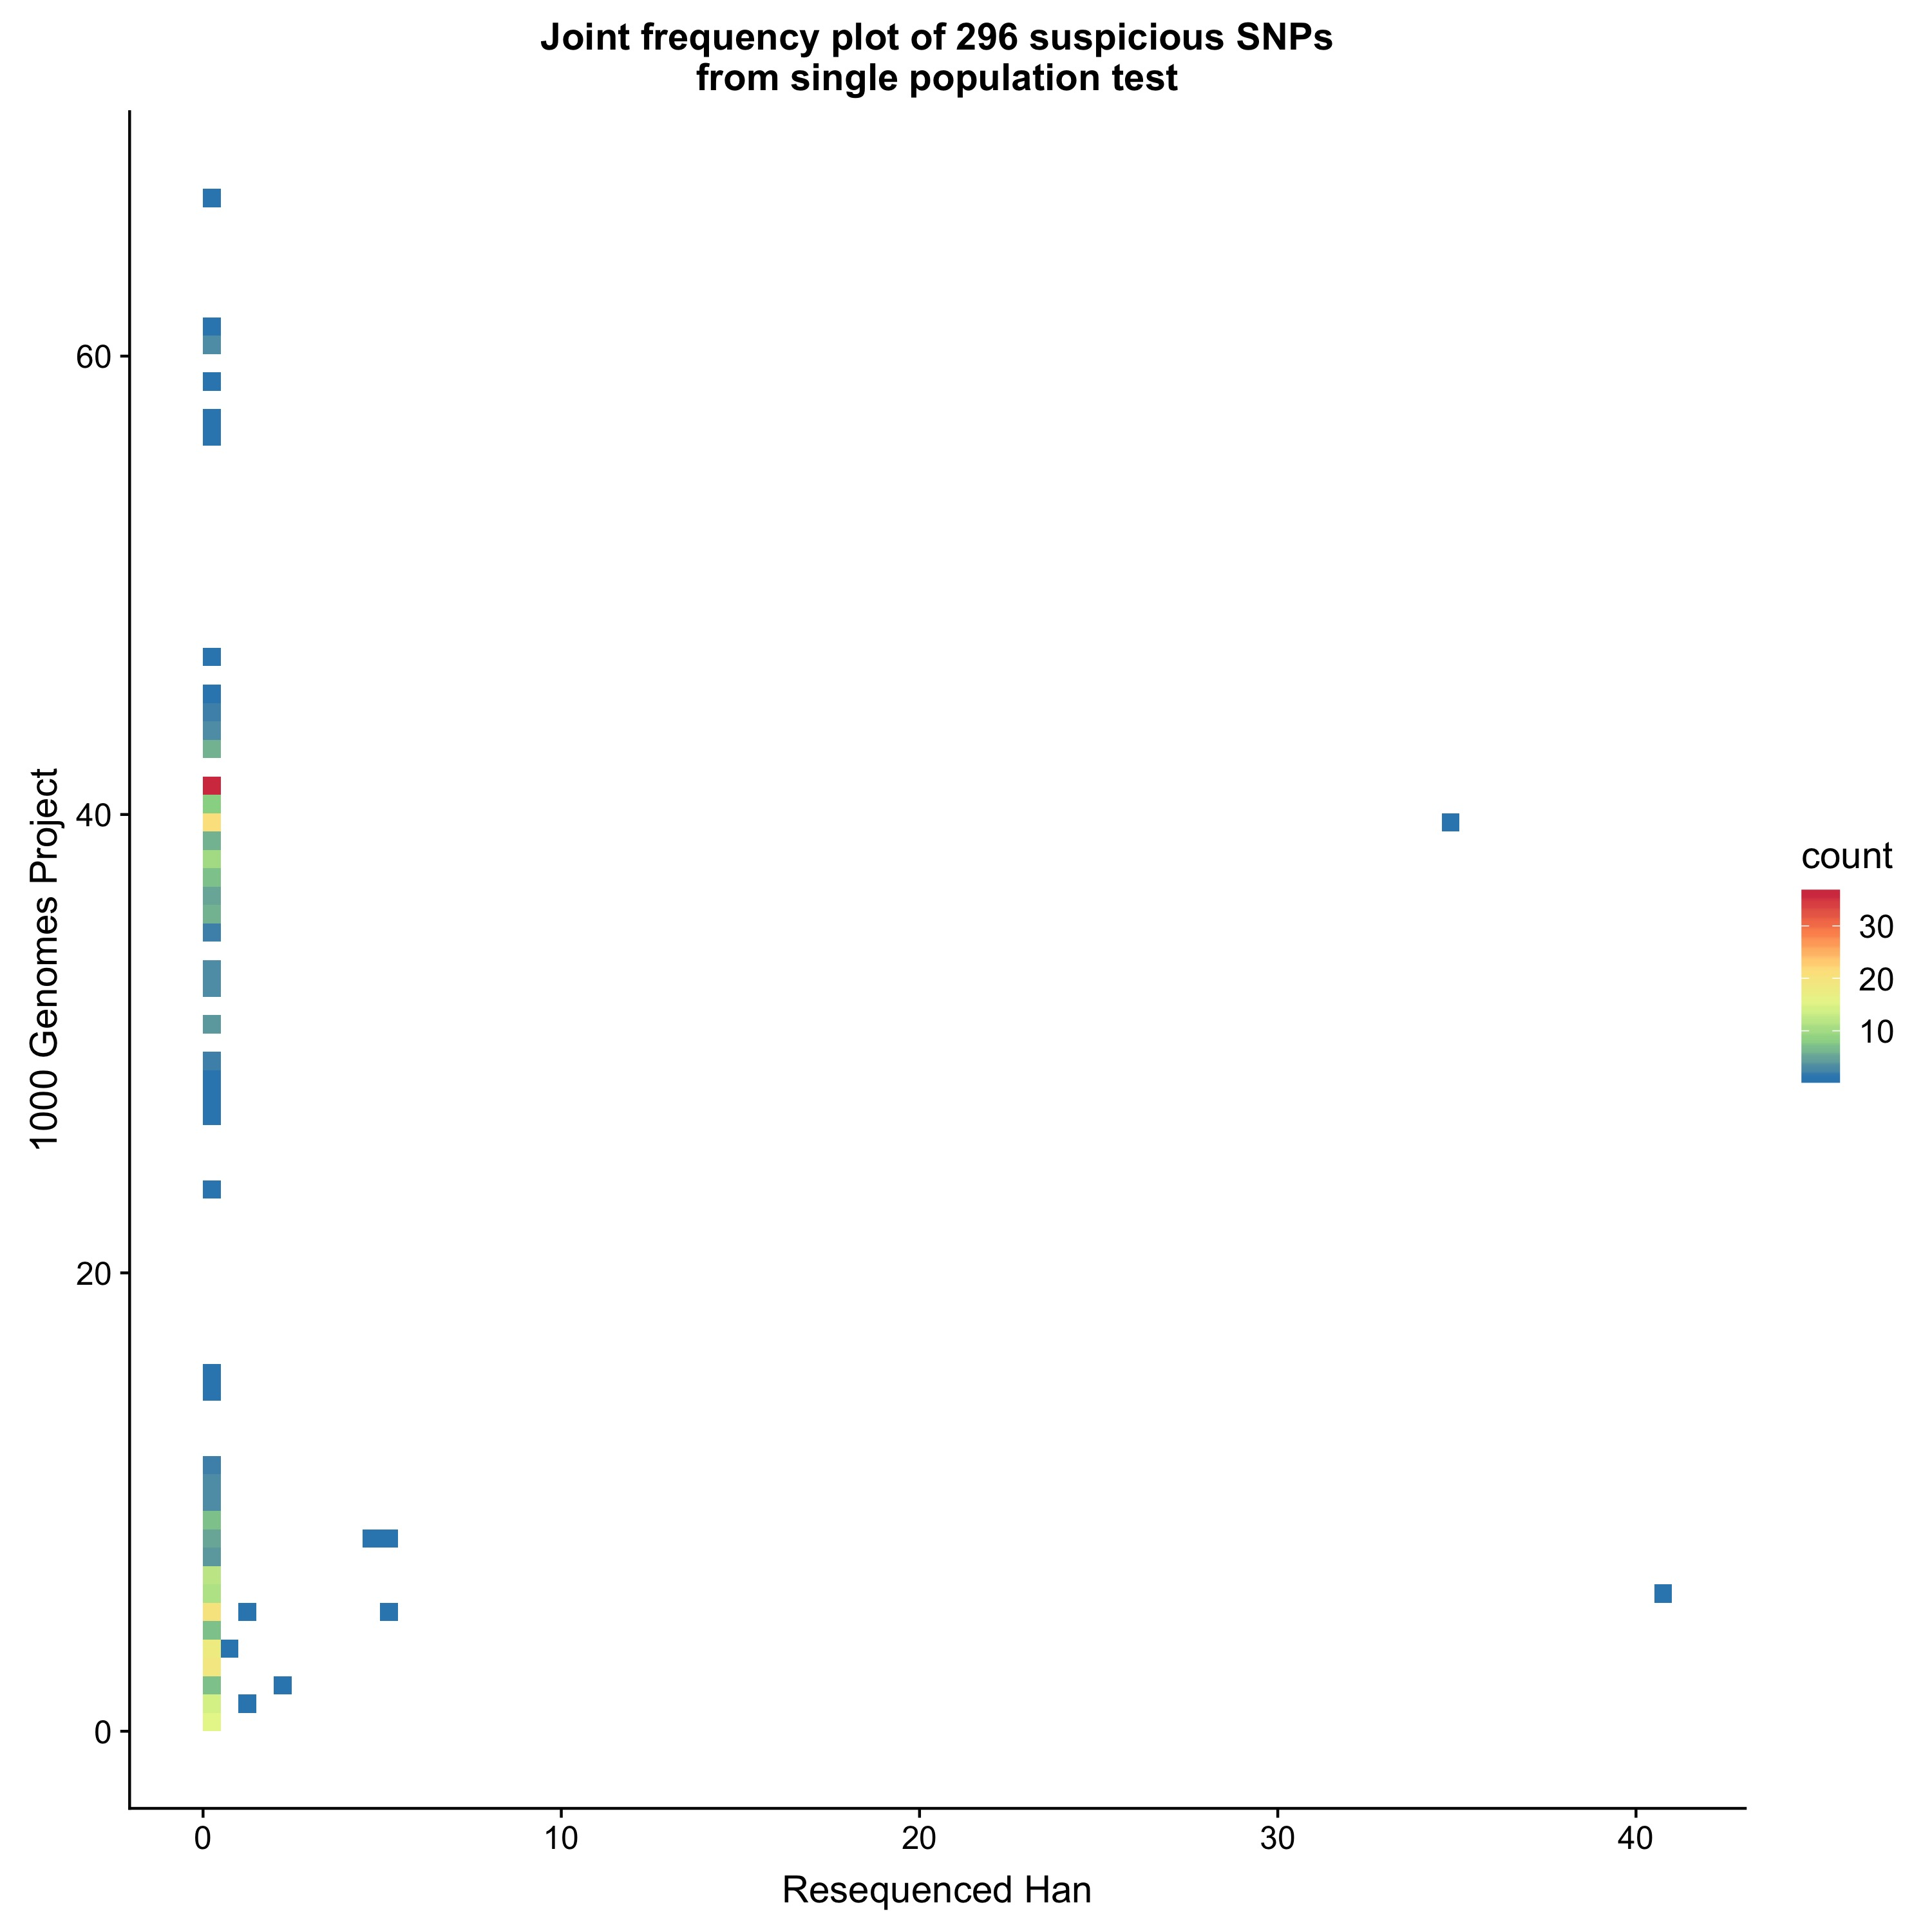
\includegraphics[width=9cm,keepaspectratio]{../Figures/Han_1kGP_SFS_singlePop.jpg}
\caption{Site frequency spectrum plot comparing the original 1000 Genomes Project data to the high depth resequence data for variants that, in the 1000 Genomes Project, are both associated with $Q$ and polymorphic in the 83 individuals that were resequenced.
Among the 296 variants associated with $Q$ in the single population tests within the 1000 Genomes Project CHB and CHS, 6 are present in the resequenced data \citep{Lan2017}.}  
\label{90HanSFS}
\end{figure}

\begin{figure}[ht]
\centering
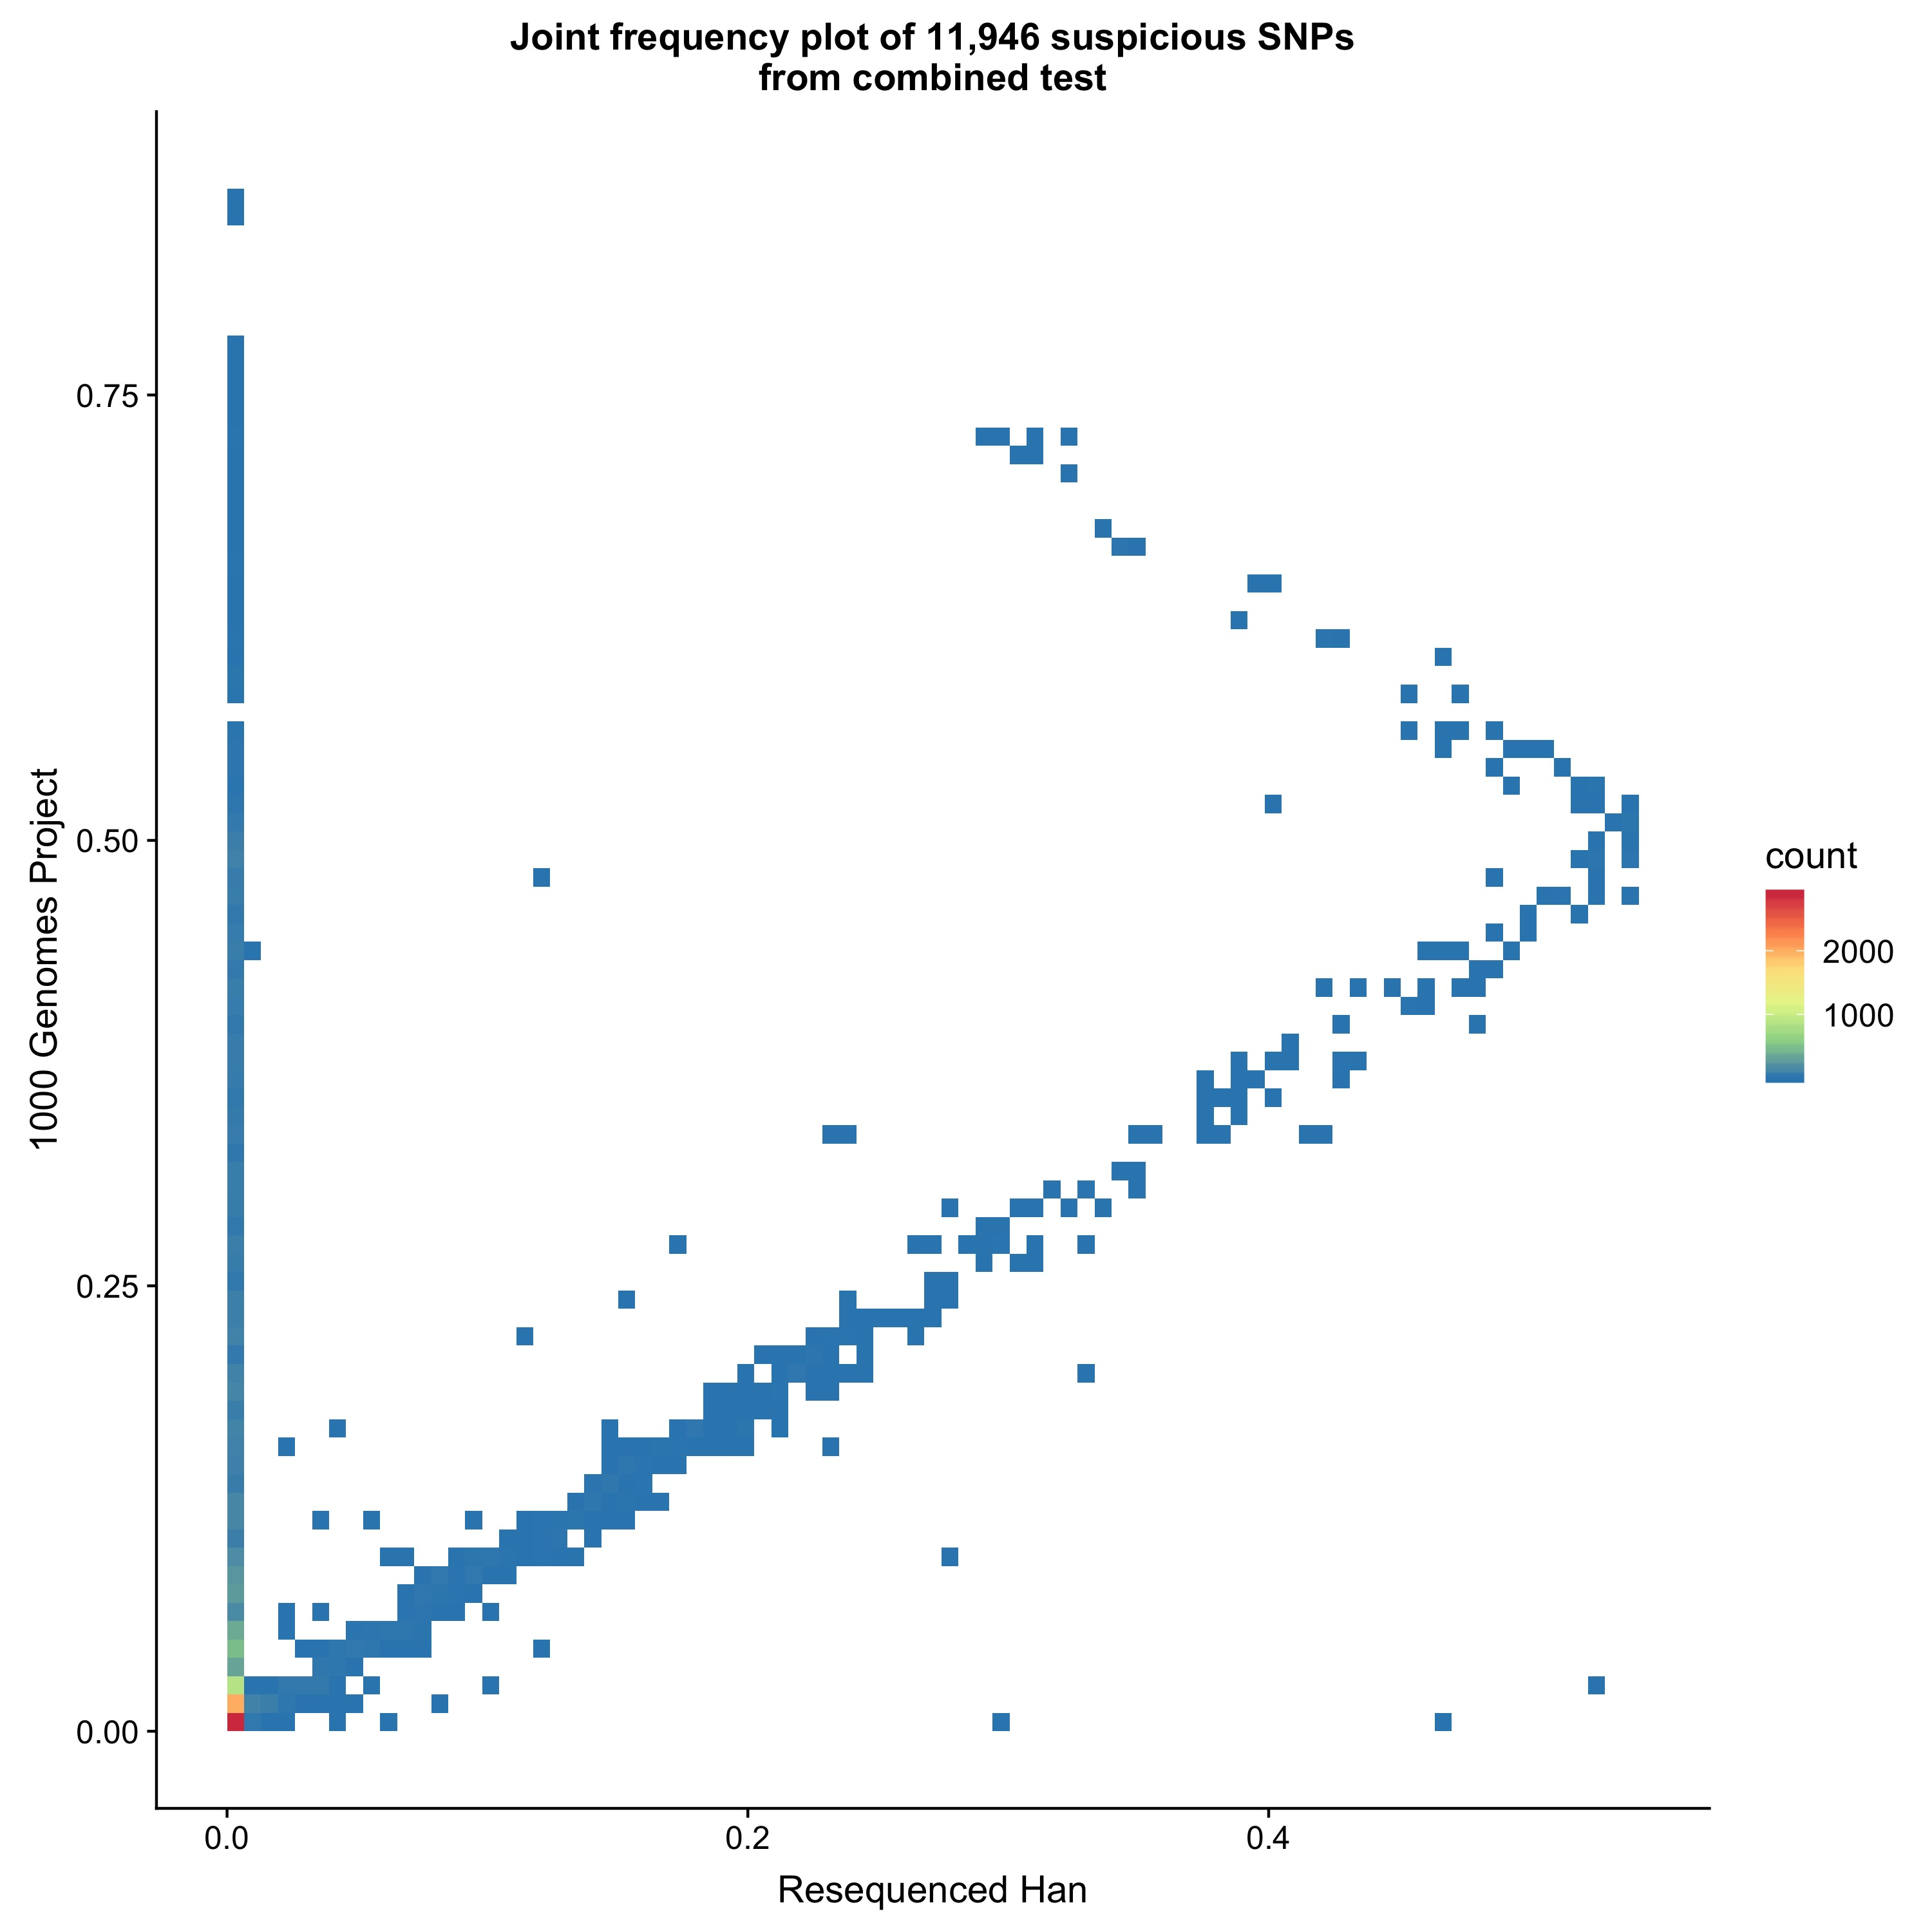
\includegraphics[width=9cm,keepaspectratio]{../Figures/Han_1kGP_SFS_FullModel.jpg}
\caption{Site frequency spectrum plot comparing the original 1000 Genomes Project data to the high depth resequence data for variants that, in the 1000 Genomes Project, are both associated with $Q$ and polymorphic in the 83 individuals that were resequenced.
Among the 6,307 variants associated with $Q$ in the GCAT model including all populations, 1,139 are present in the high depth resequenced individuals.}  
\label{90HanSFS_30}
\end{figure}

\begin{figure} \centering
    \begin{subfigure}[b]{\linewidth}
        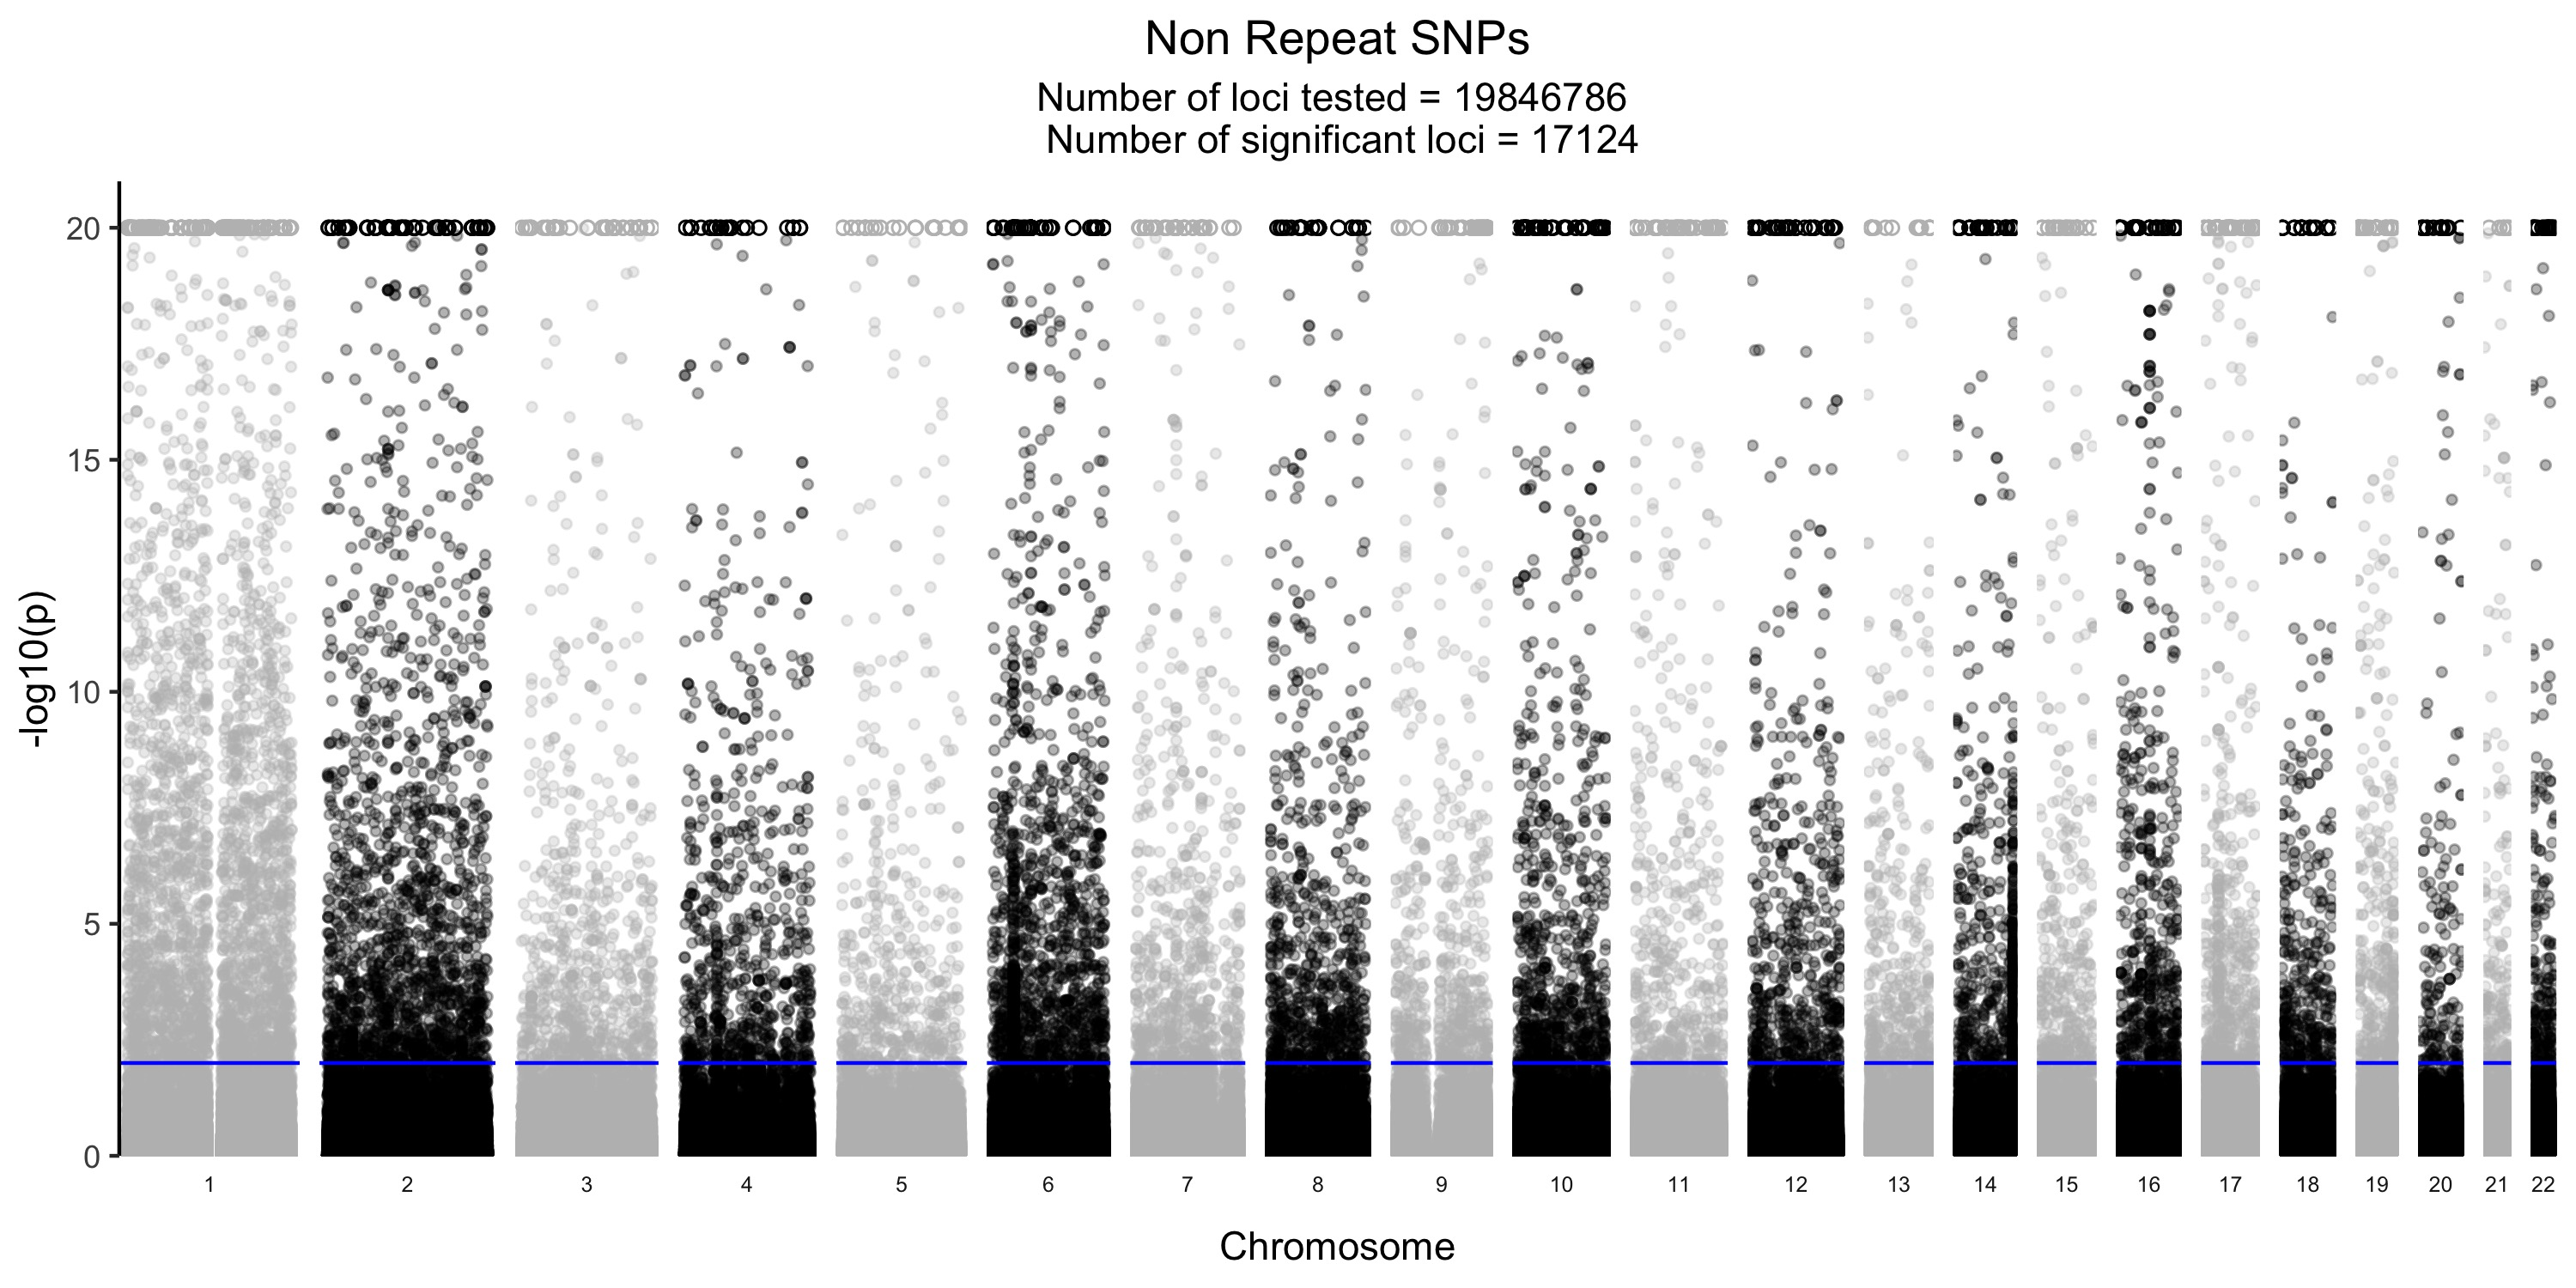
\includegraphics[width=\hsize]{../Figures/ManhattanPlot_NonRepeatSNPs.jpg}
    \end{subfigure} 
    \begin{subfigure}[b]{\linewidth}
    	\center    
        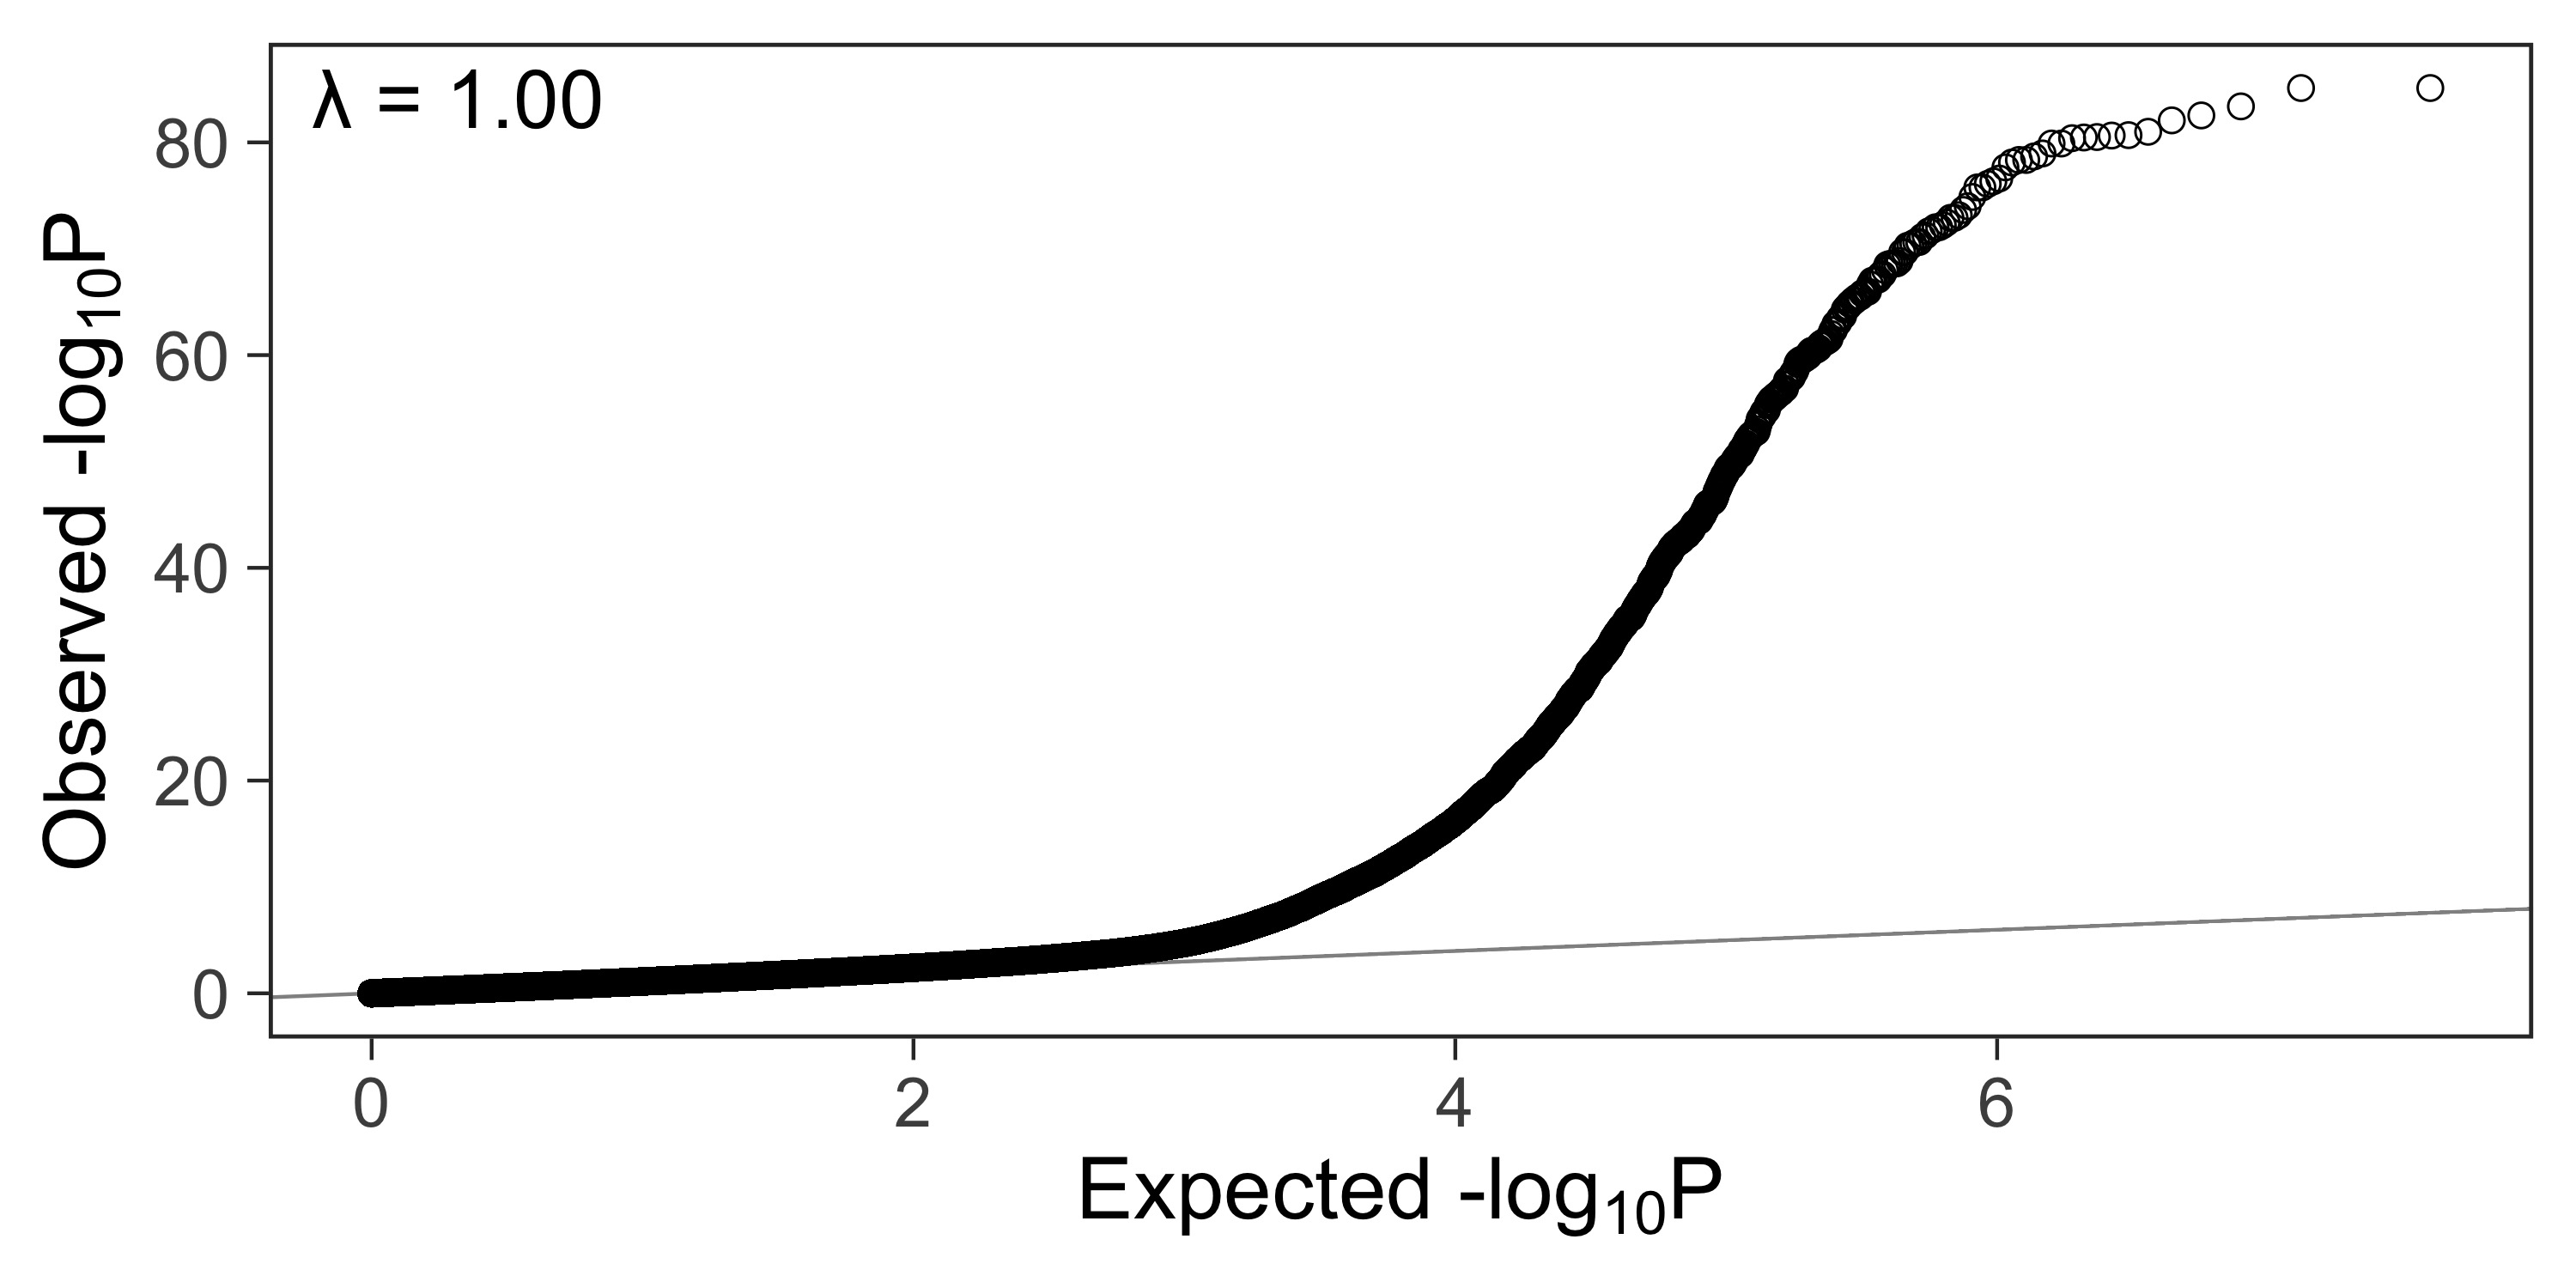
\includegraphics[width=\hsize]{../Figures/QQPlot_NonRepeatSNPs.jpg}
    
    \end{subfigure} 
    \caption{Association of SNPS in non-repetitive regions with $Q$.
    \textbf{A} Manhattan plot of the $-\log_{10}(p)$ values for the reverse GWAS logistic regression analysis for SNPs in non repetitive regions. There are 15,018 SNPs that reach $p$ values greater than $ p < 0.01$ after performing a two-stage Benjamini and Hochberg FDR adjustment.  The circles ( o ) are variants that reached values greater than 20, for clarity we implemented hard ceiling at 20. 
  \textbf{B} QQ plot of the unadjusted p values for the reverse GWAS logistic regression analysis for SNPs in non repetitive regions.}
  \label{NRS_Manhattan}
  \end{figure}
\begin{figure} \centering
    \begin{subfigure}[b]{\linewidth}
        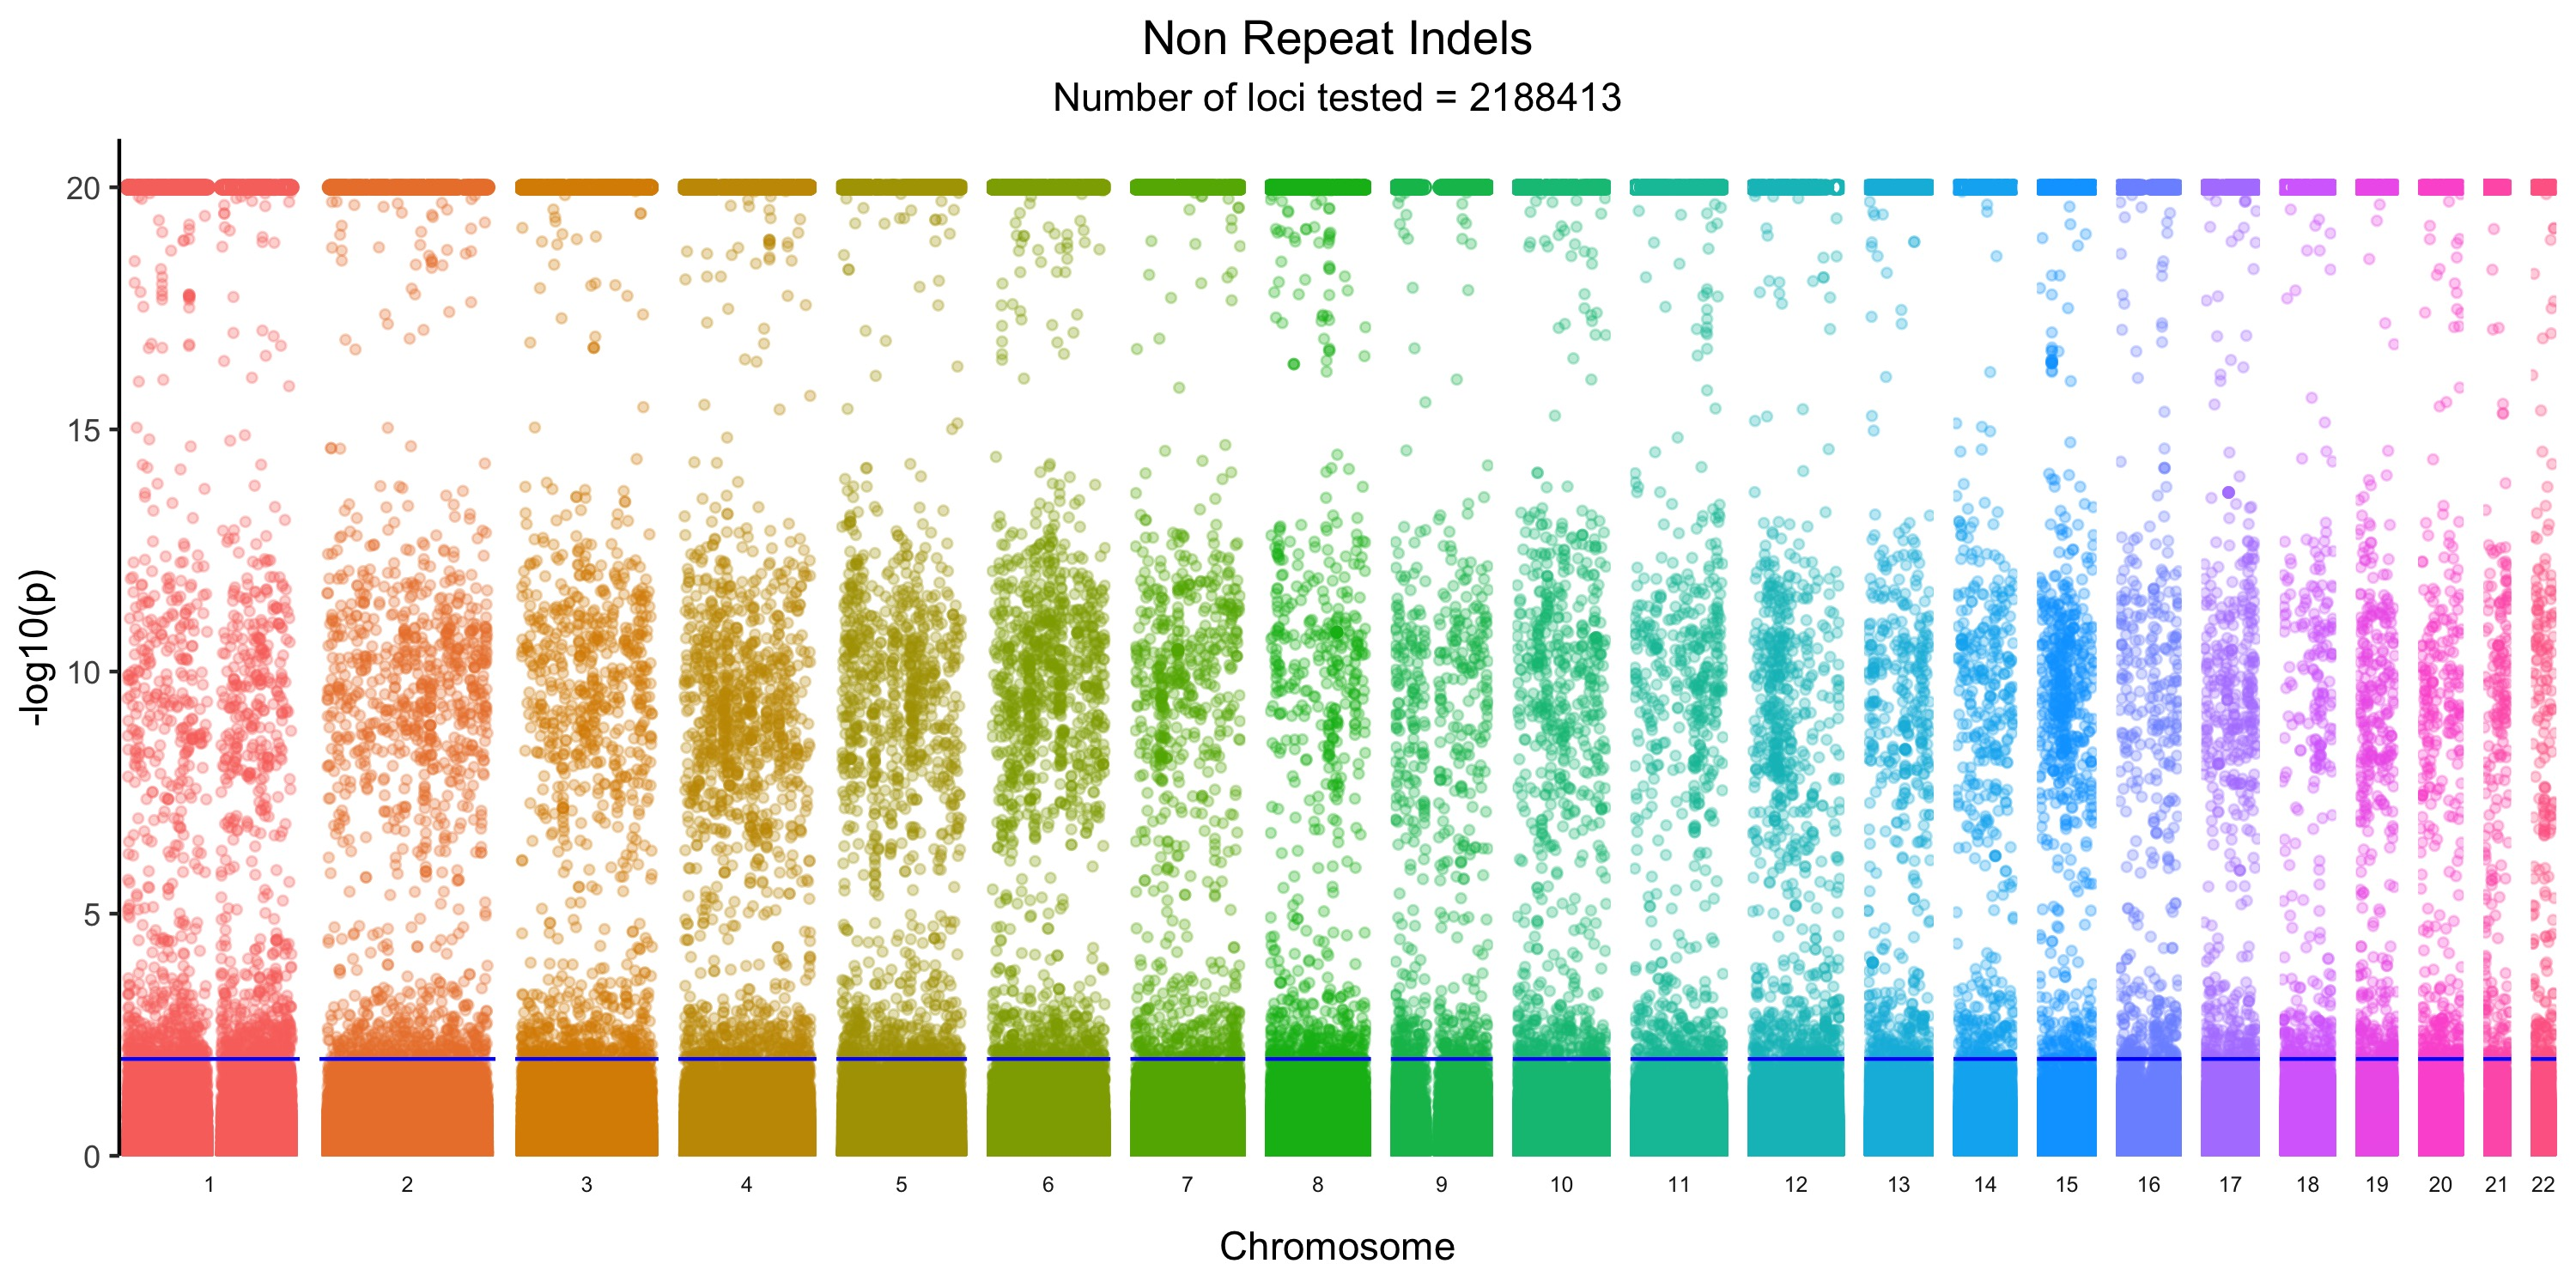
\includegraphics[width=\hsize]{../Figures/ManhattanPlot_NonRepeatIndels.jpg}
    \end{subfigure} %
    \begin{subfigure}[b]{\linewidth}
    	\center    
        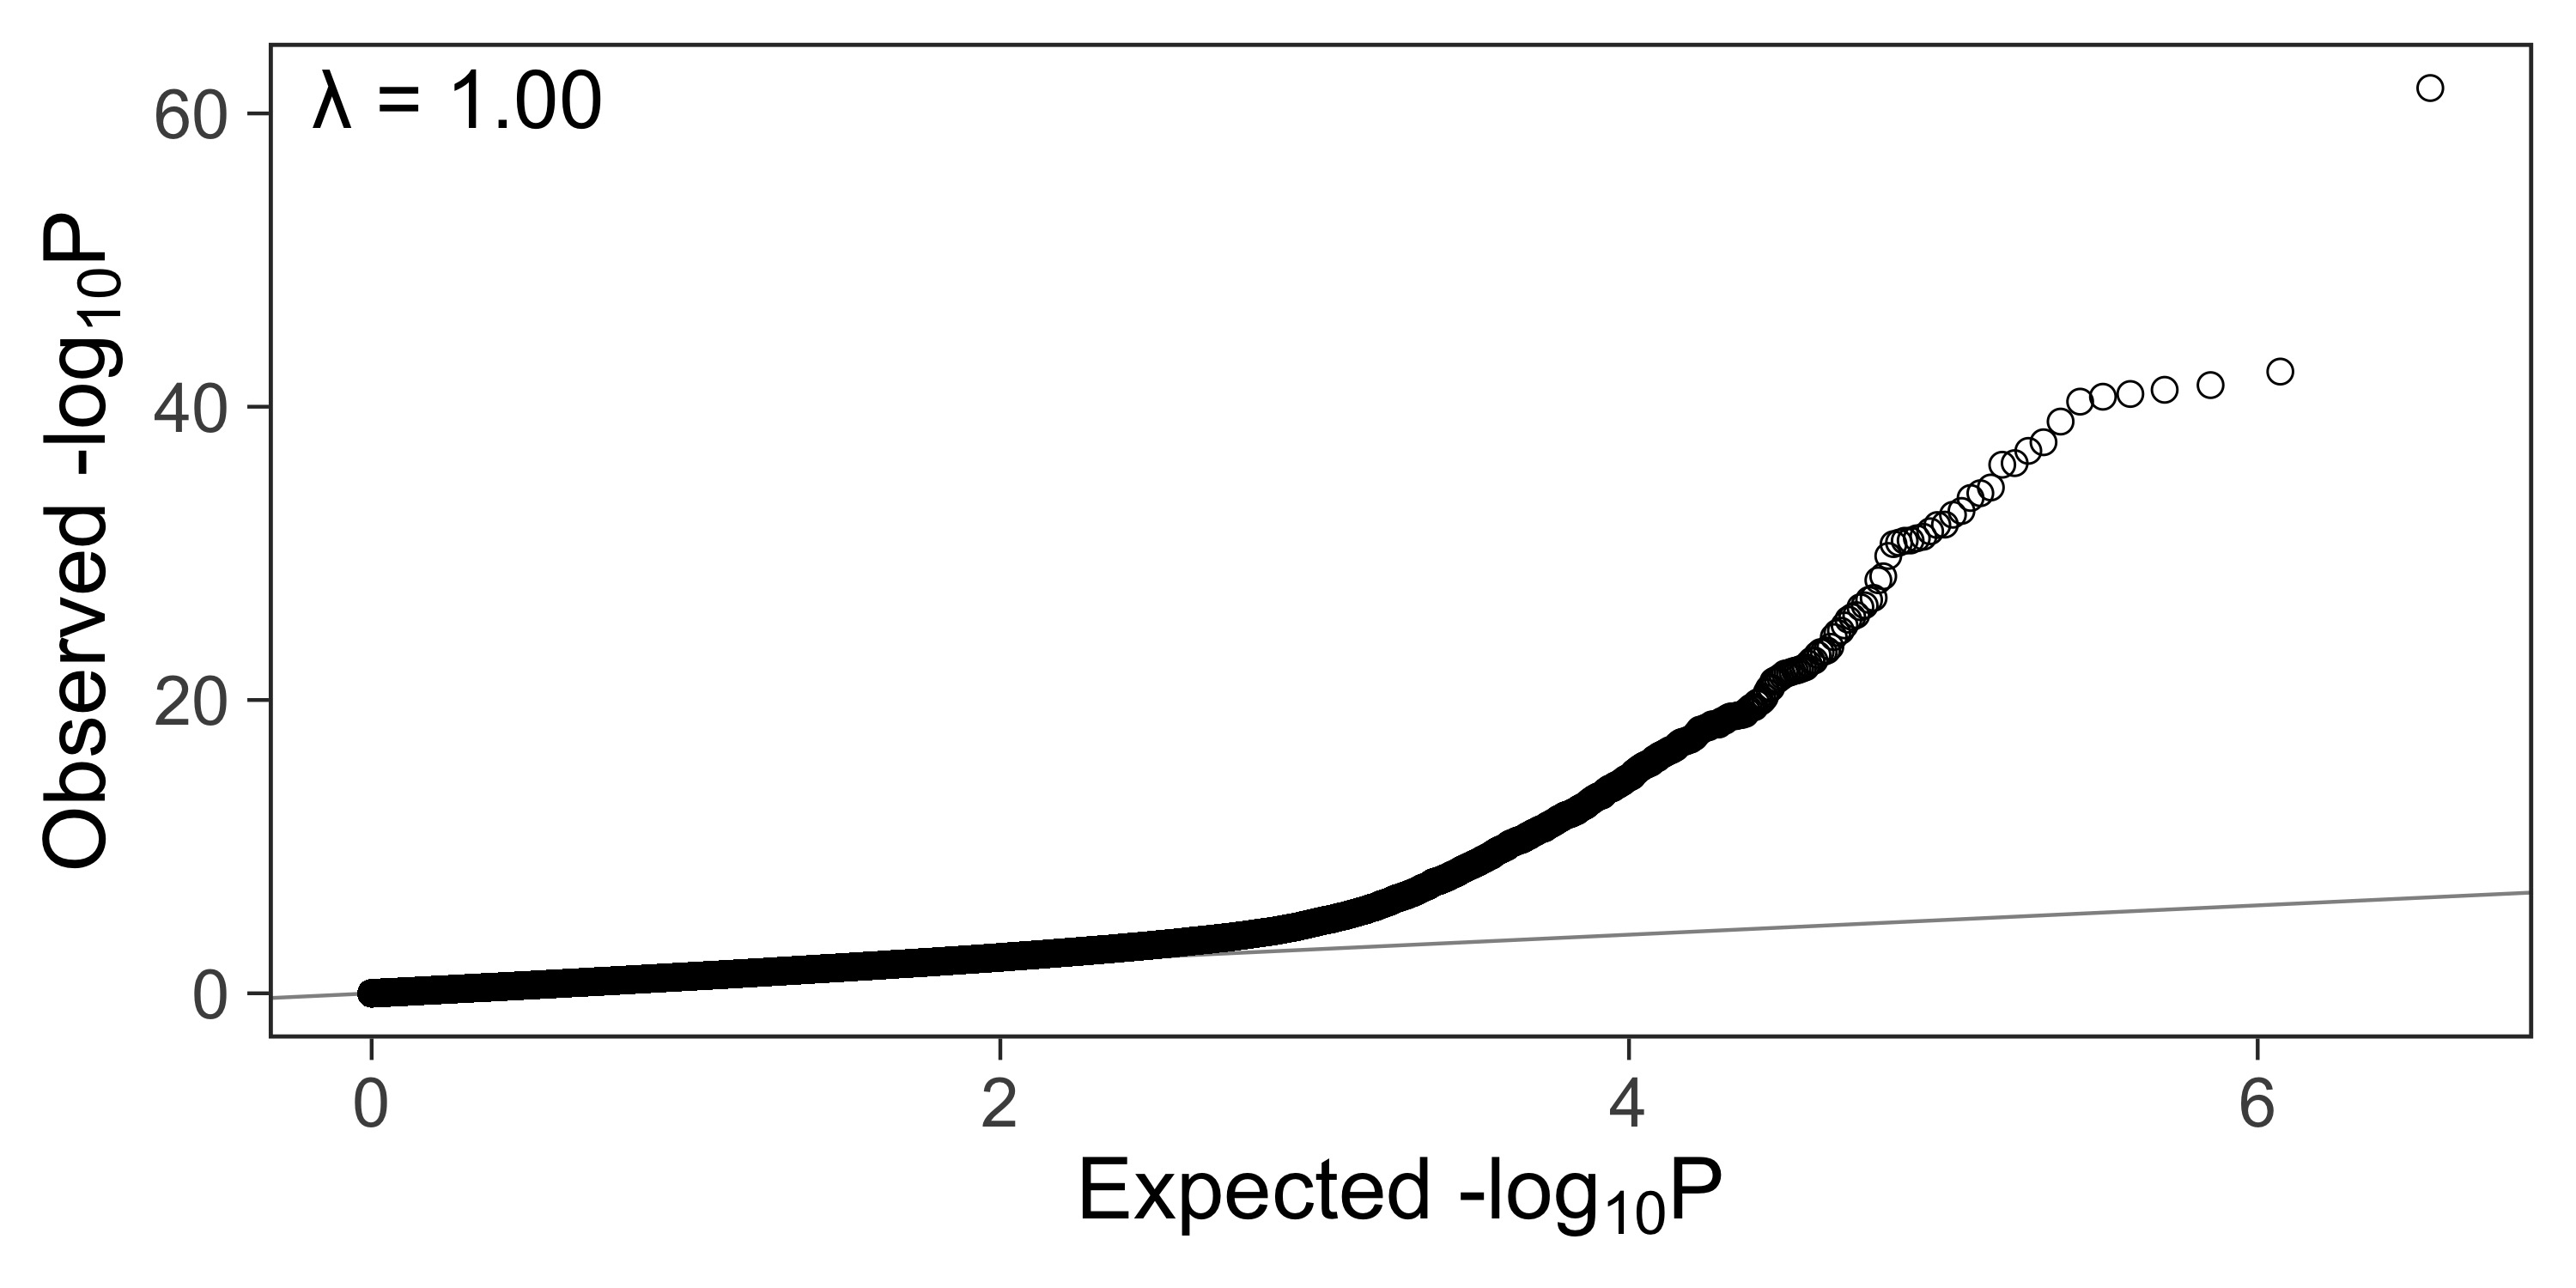
\includegraphics[width=\hsize]{../Figures/QQPlot_NonRepeatIndels.jpg}
    
    \end{subfigure} 
    \caption{Association of indels in non-repetitive regions with $Q$. \textbf{A} Manhattan plot of the $-\log_{10}(p)$ values for the reverse GWAS logistic regression analysis for INDELs in non repetitive regions. There are 2,121 INDELs that reach $p$ values greater than $ p < 0.01$ after performing a two-stage Benjamini and Hochberg FDR adjustment.  The circles ( o ) are variants that reached values greater than 20, for clarity we implemented hard ceiling at 20. 
  \textbf{B} QQ plot of the unadjusted p values for the reverse GWAS logistic regression analysis for INDELs in non repetitive regions.}
  \label{NRI_Manhattan}
  \end{figure}
\begin{figure} \centering
    \begin{subfigure}[b]{\linewidth}
        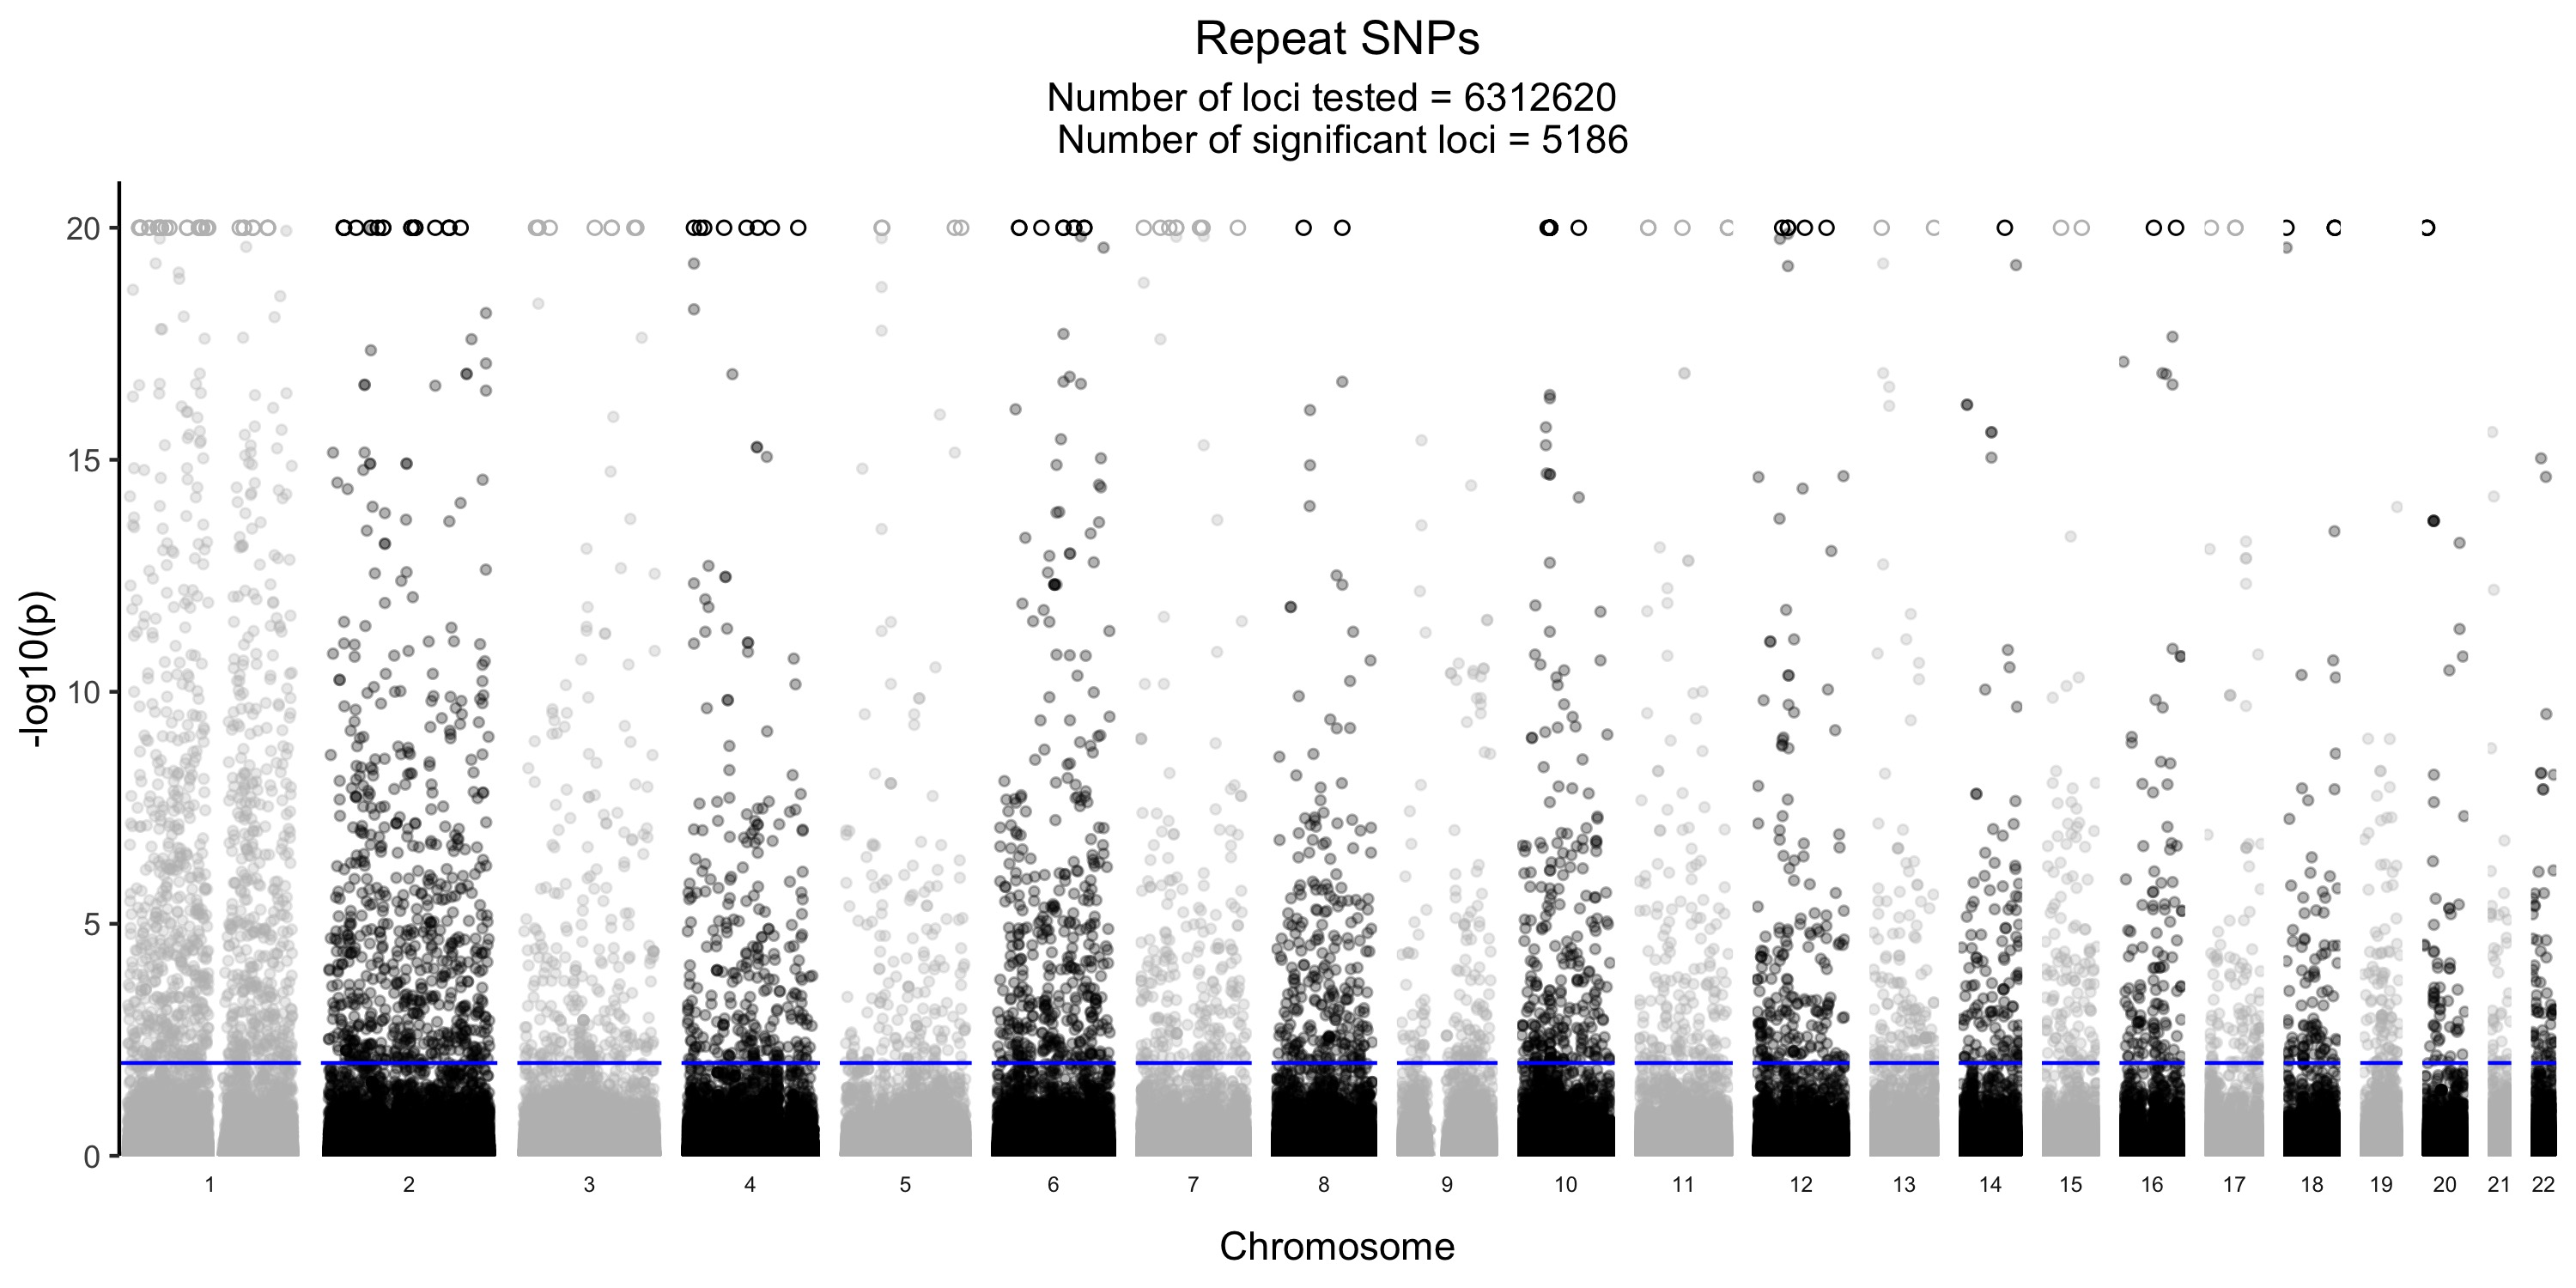
\includegraphics[width=\hsize]{../Figures/ManhattanPlot_RepeatSNPs.jpg}
    \end{subfigure} %
    \begin{subfigure}[b]{\linewidth}
    	\center    
        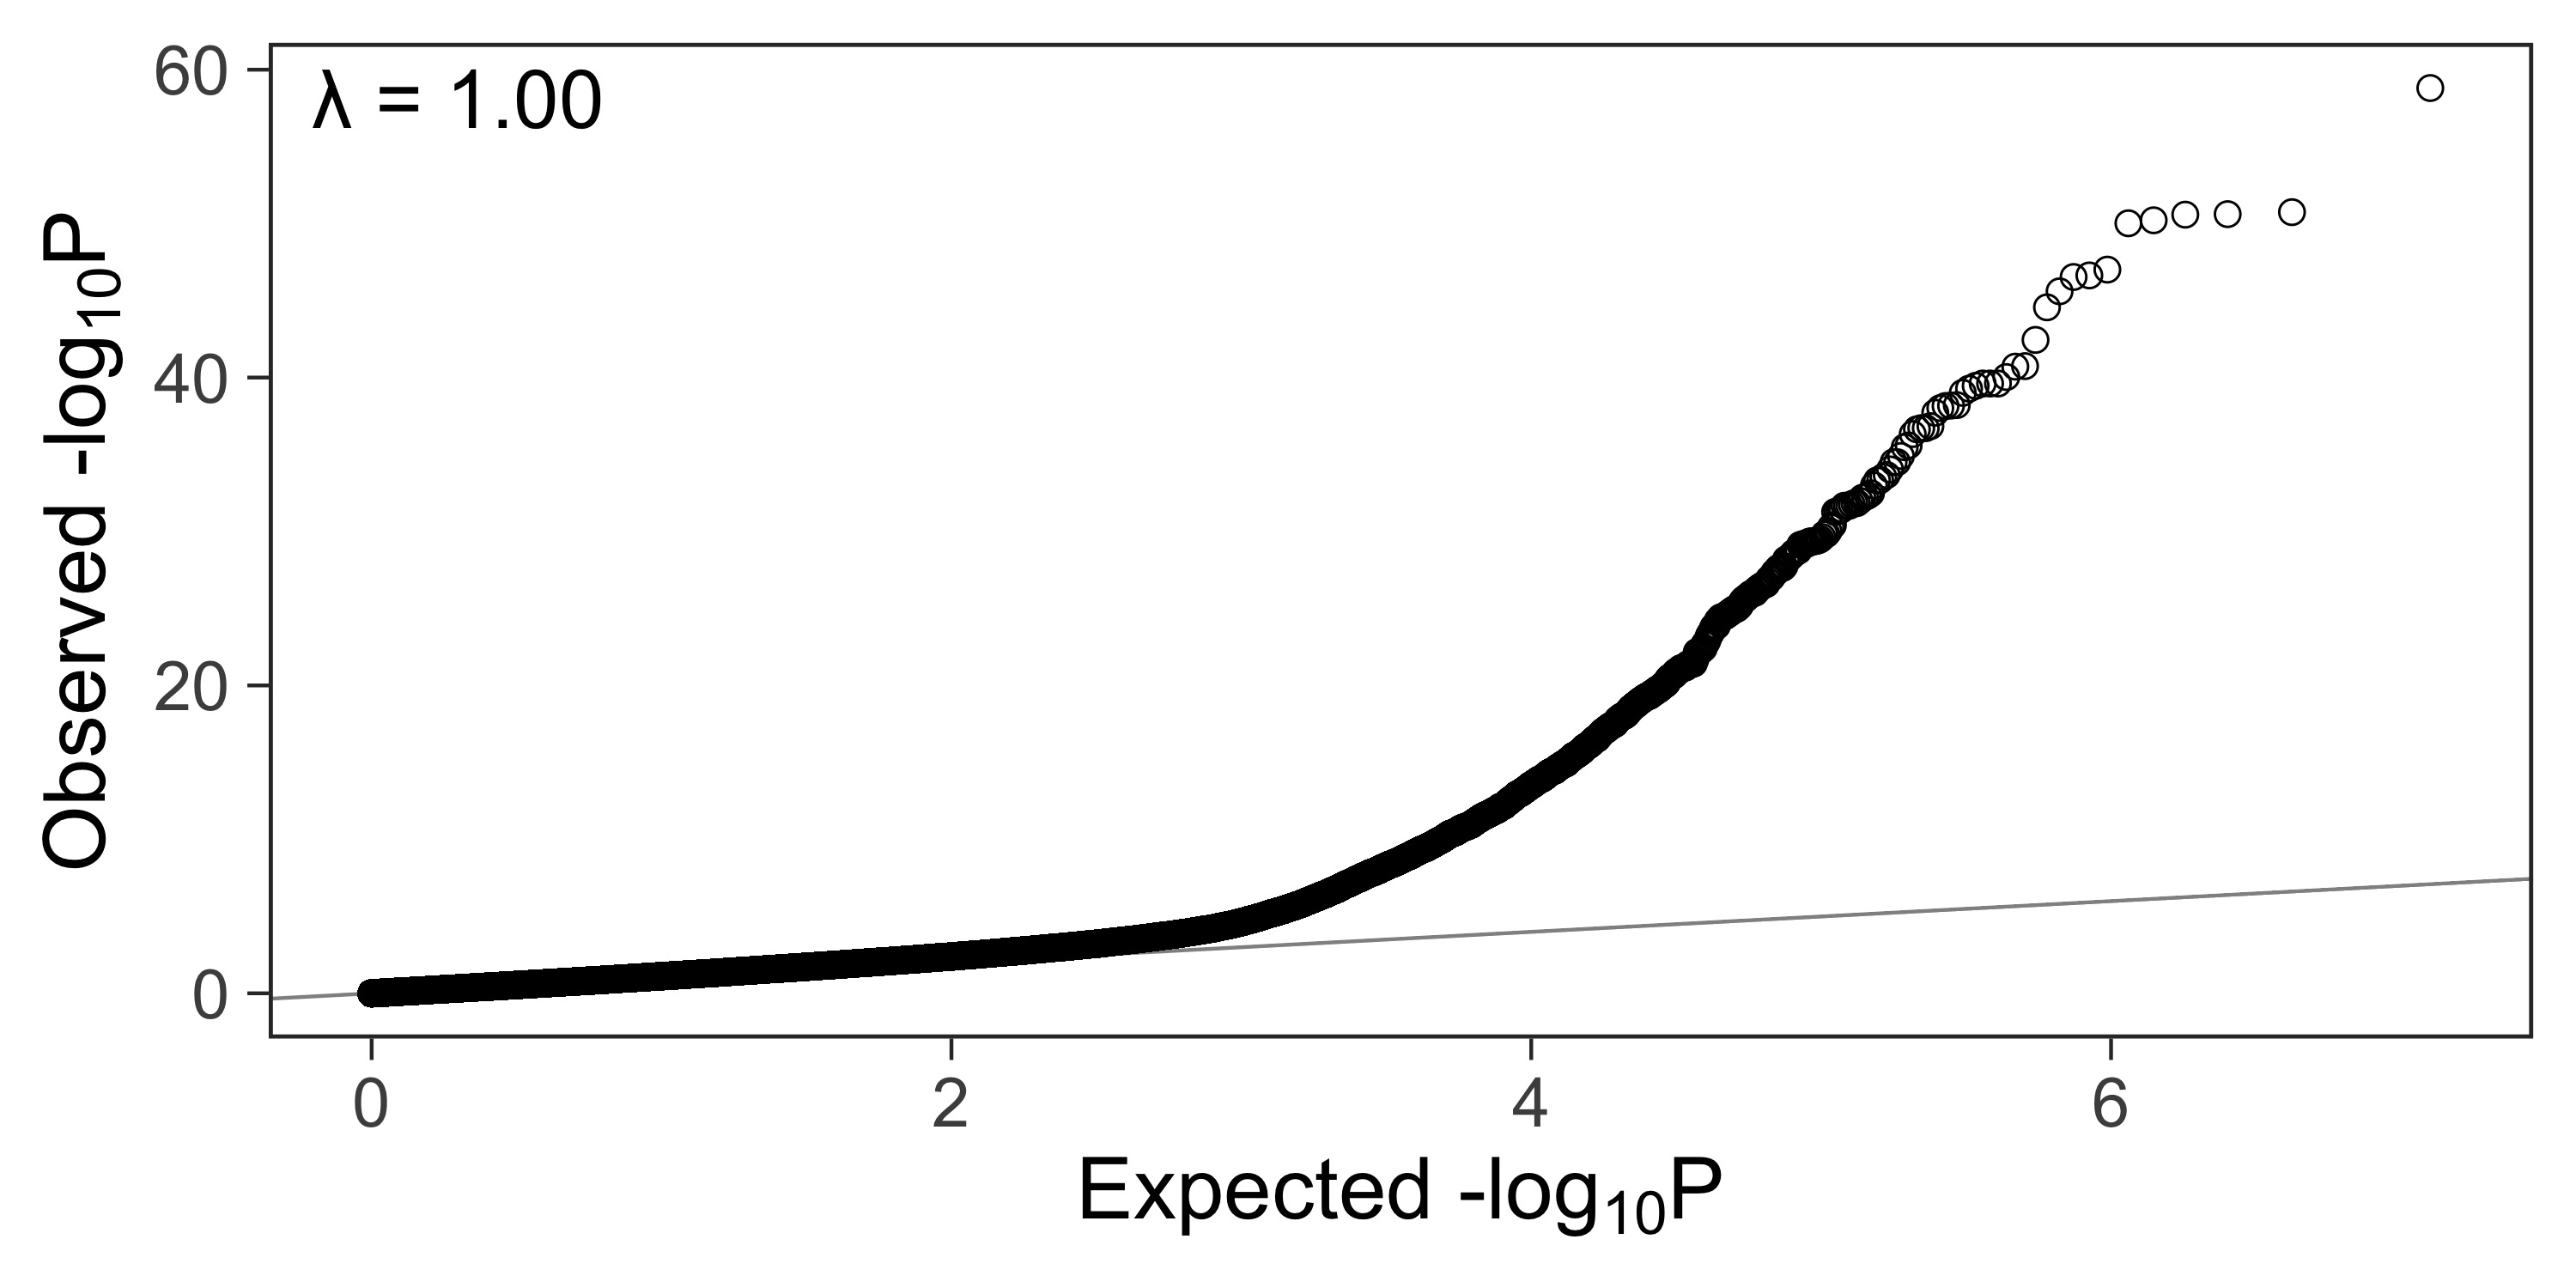
\includegraphics[width=\hsize]{../Figures/QQPlot_RepeatSNPs.jpg}
    
    \end{subfigure} 
    \caption{Association of SNPS in repetitive regions with $Q$. \textbf{A} Manhattan plot of the $-\log_{10}(p)$ values for the reverse GWAS logistic regression analysis for SNPs in repetitive regions. There are 4,405 SNPs that reach $p$ values greater than $ p < 0.01$ after performing a two-stage Benjamini and Hochberg FDR adjustment.  The circles ( o ) are variants that reached values greater than 20, for clarity we implemented hard ceiling at 20. 
  \textbf{B} QQ plot of the unadjusted p values for the reverse GWAS logistic regression analysis for SNPs in repetitive regions.}
  \label{RS_Manhattan}
  \end{figure}
\begin{figure} \centering
    \begin{subfigure}[b]{\linewidth}
        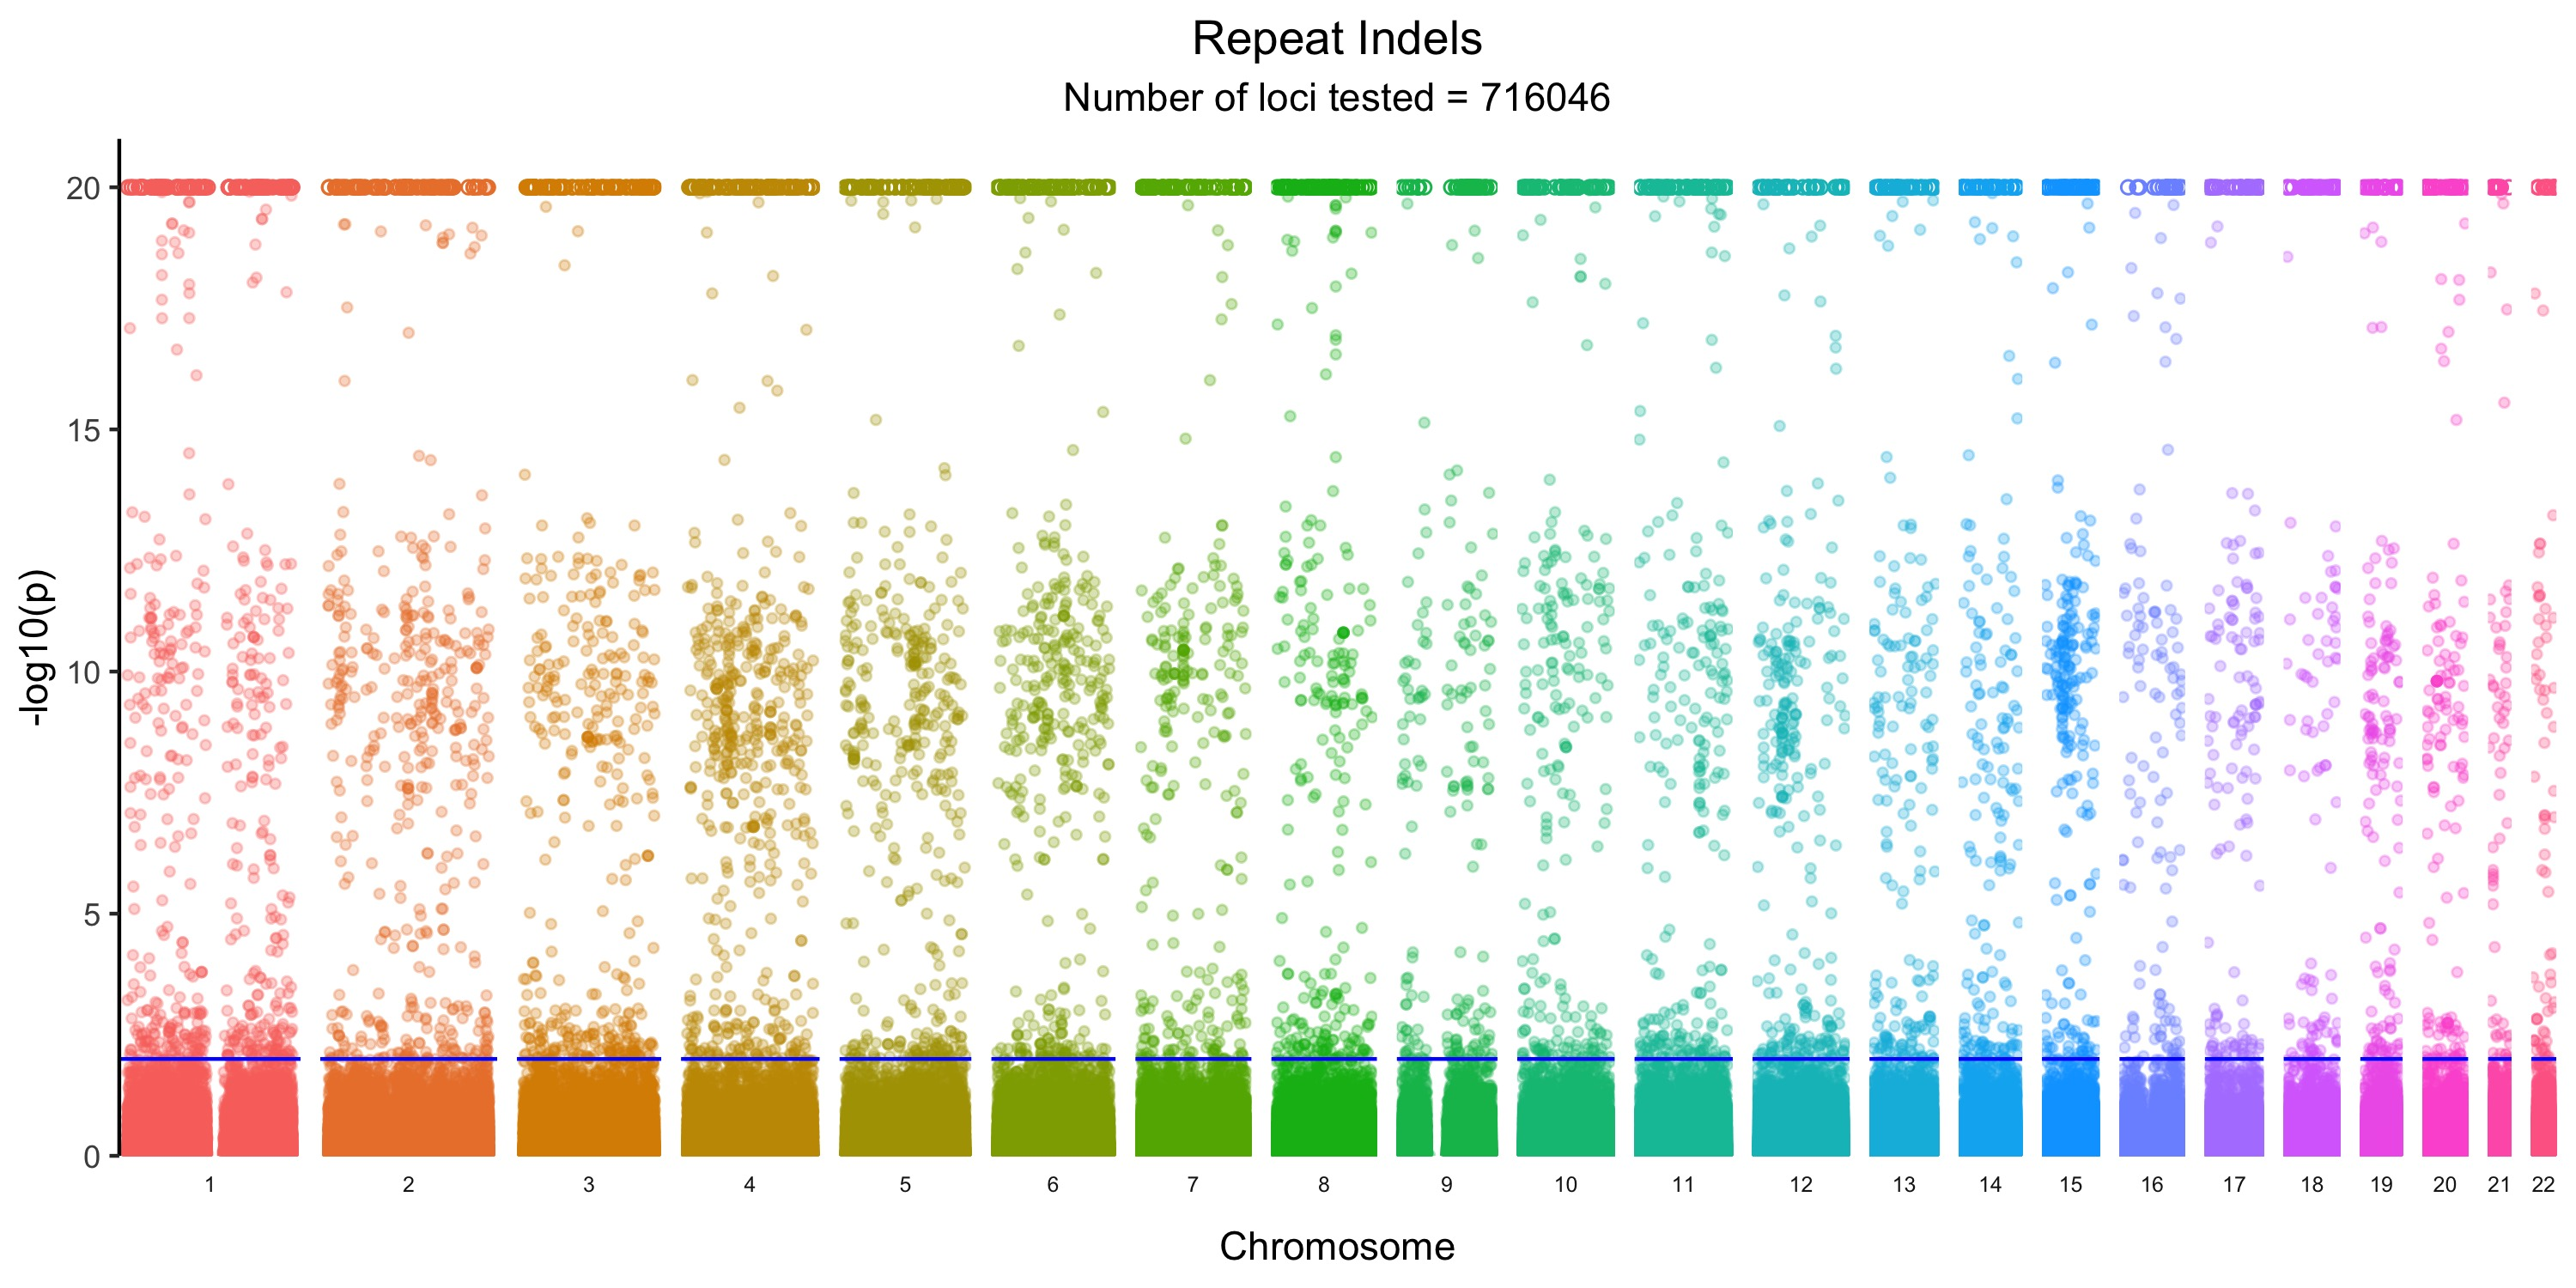
\includegraphics[width=\hsize]{../Figures/ManhattanPlot_RepeatIndels.jpg}
    \end{subfigure} %
    \begin{subfigure}[b]{\linewidth}
    	\center    
        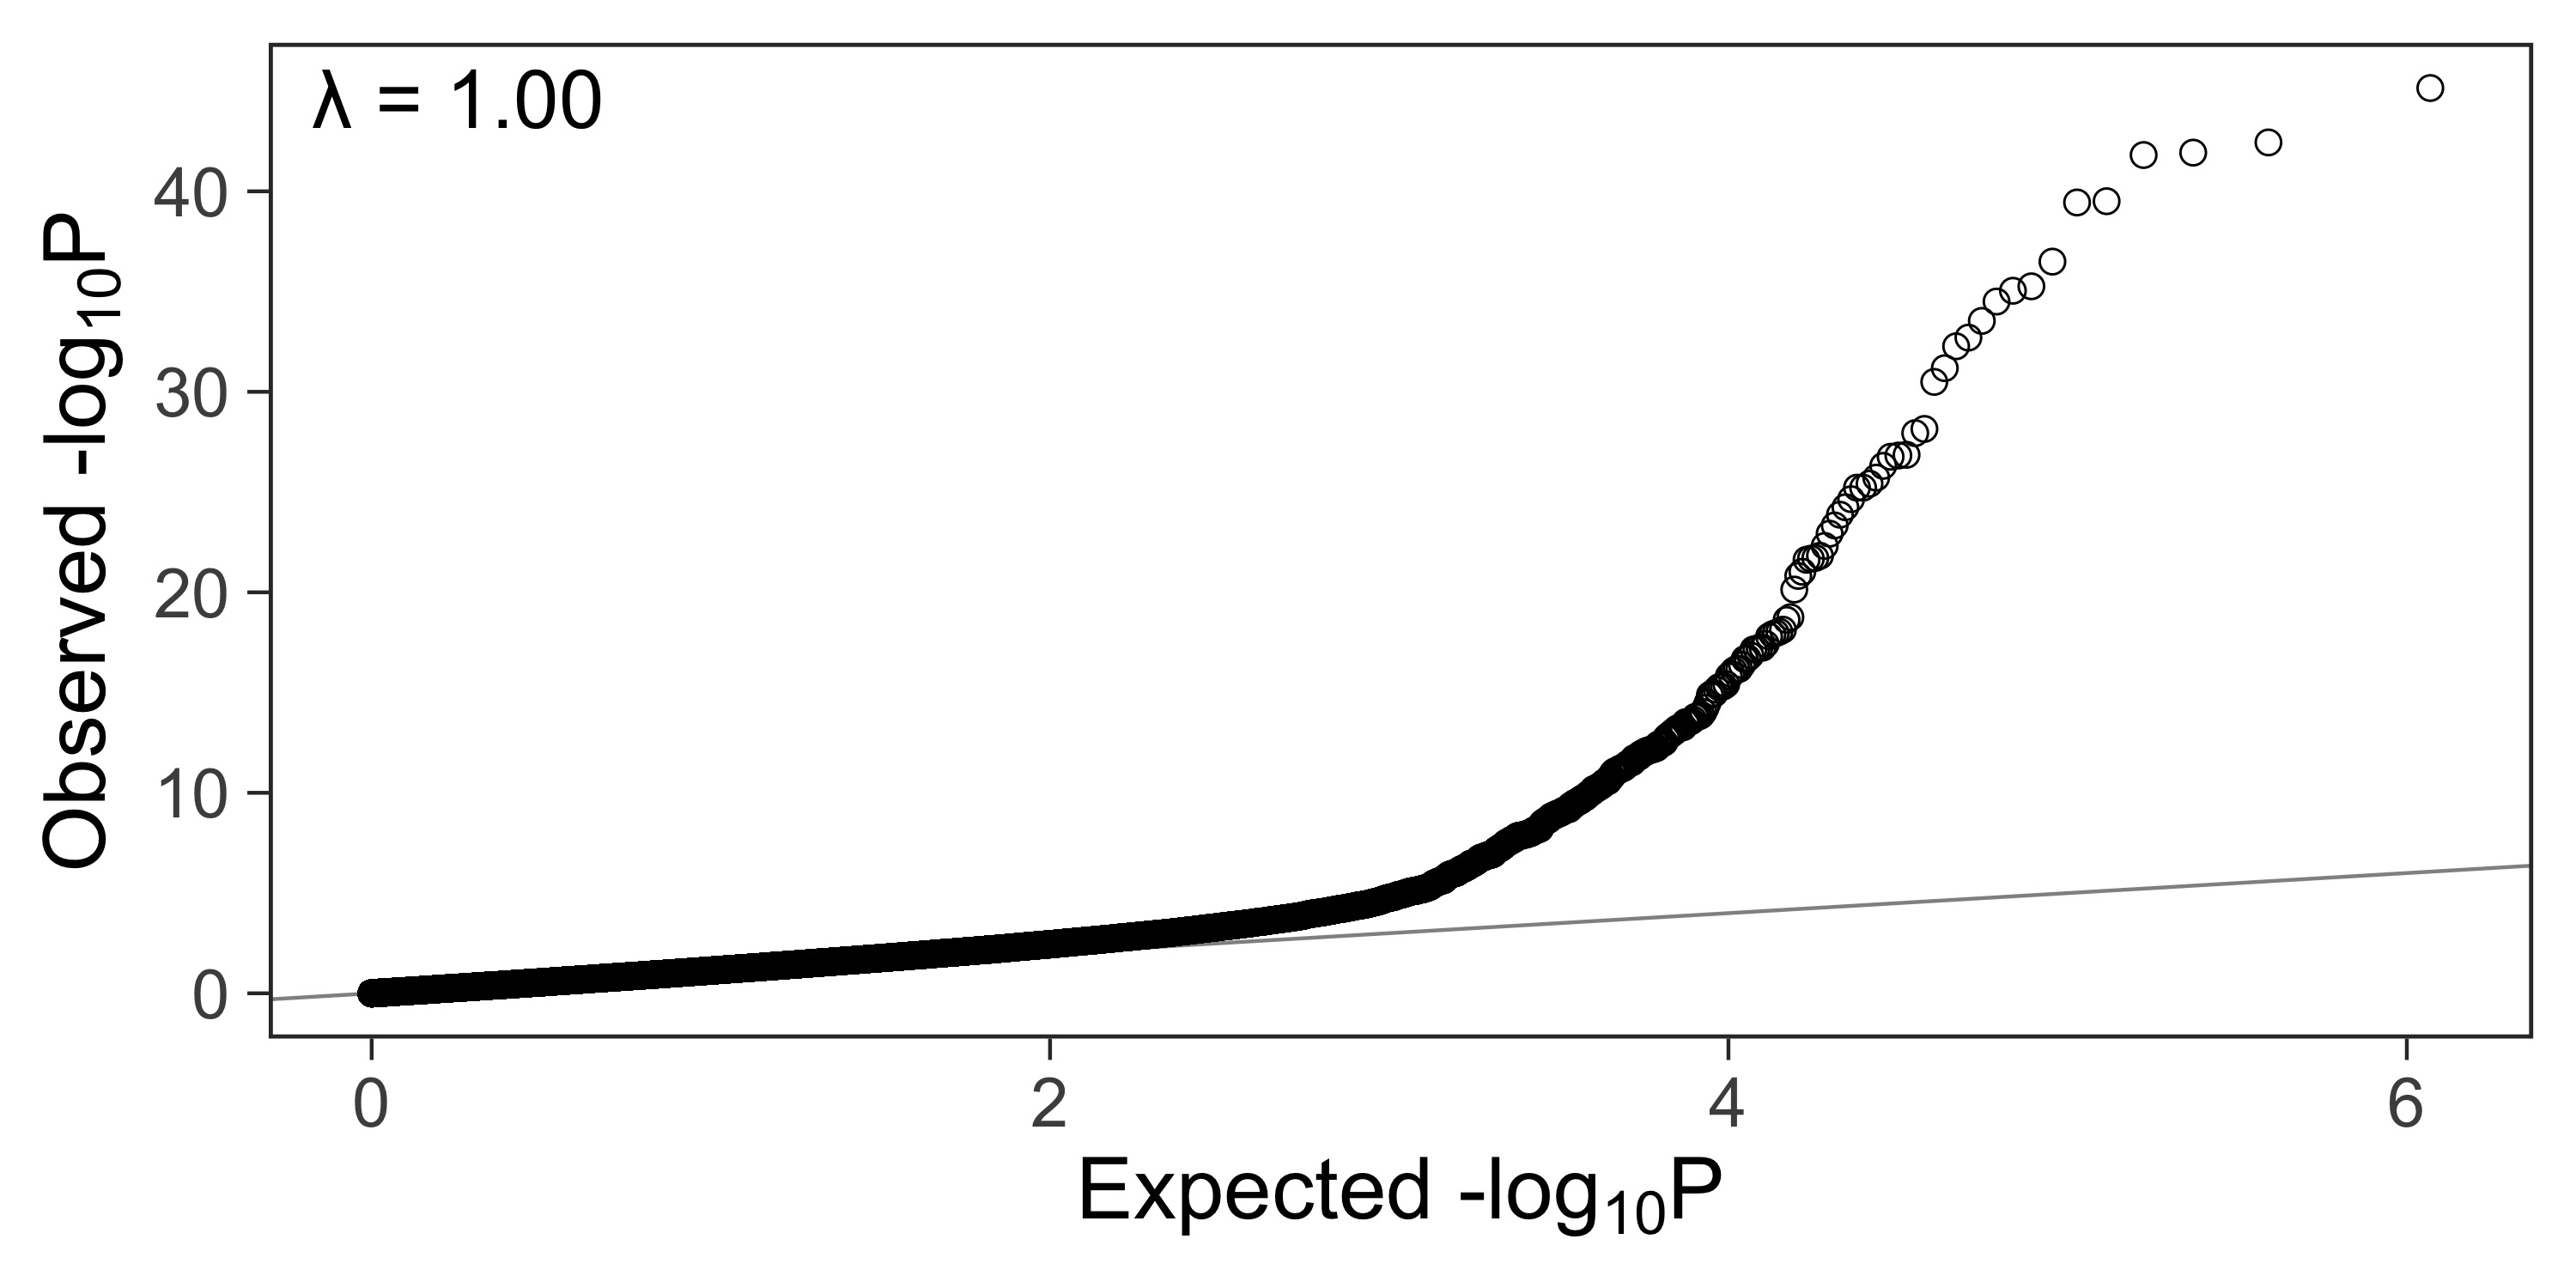
\includegraphics[width=\hsize]{../Figures/QQPlot_RepeatIndels.jpg}
    \end{subfigure} 
    \caption{Association of indels in repetitive regions with $Q$.  \textbf{A} Manhattan plot of the $-\log_{10}(p)$ values for the reverse GWAS logistic regression analysis for INDELs in repetitive regions. There are 642 INDELs that reach $p$ values greater than $ p < 0.01$ after performing a two-stage Benjamini and Hochberg FDR adjustment.  The circles ( o ) are variants that reached values greater than 20, for clarity we implemented hard ceiling at 20. 
  \textbf{B} QQ plot of the unadjusted p values for the reverse GWAS logistic regression analysis for INDELs in repetitive regions.}
  \label{RI_Manhattan}
  \end{figure}

\begin{figure}[ht]
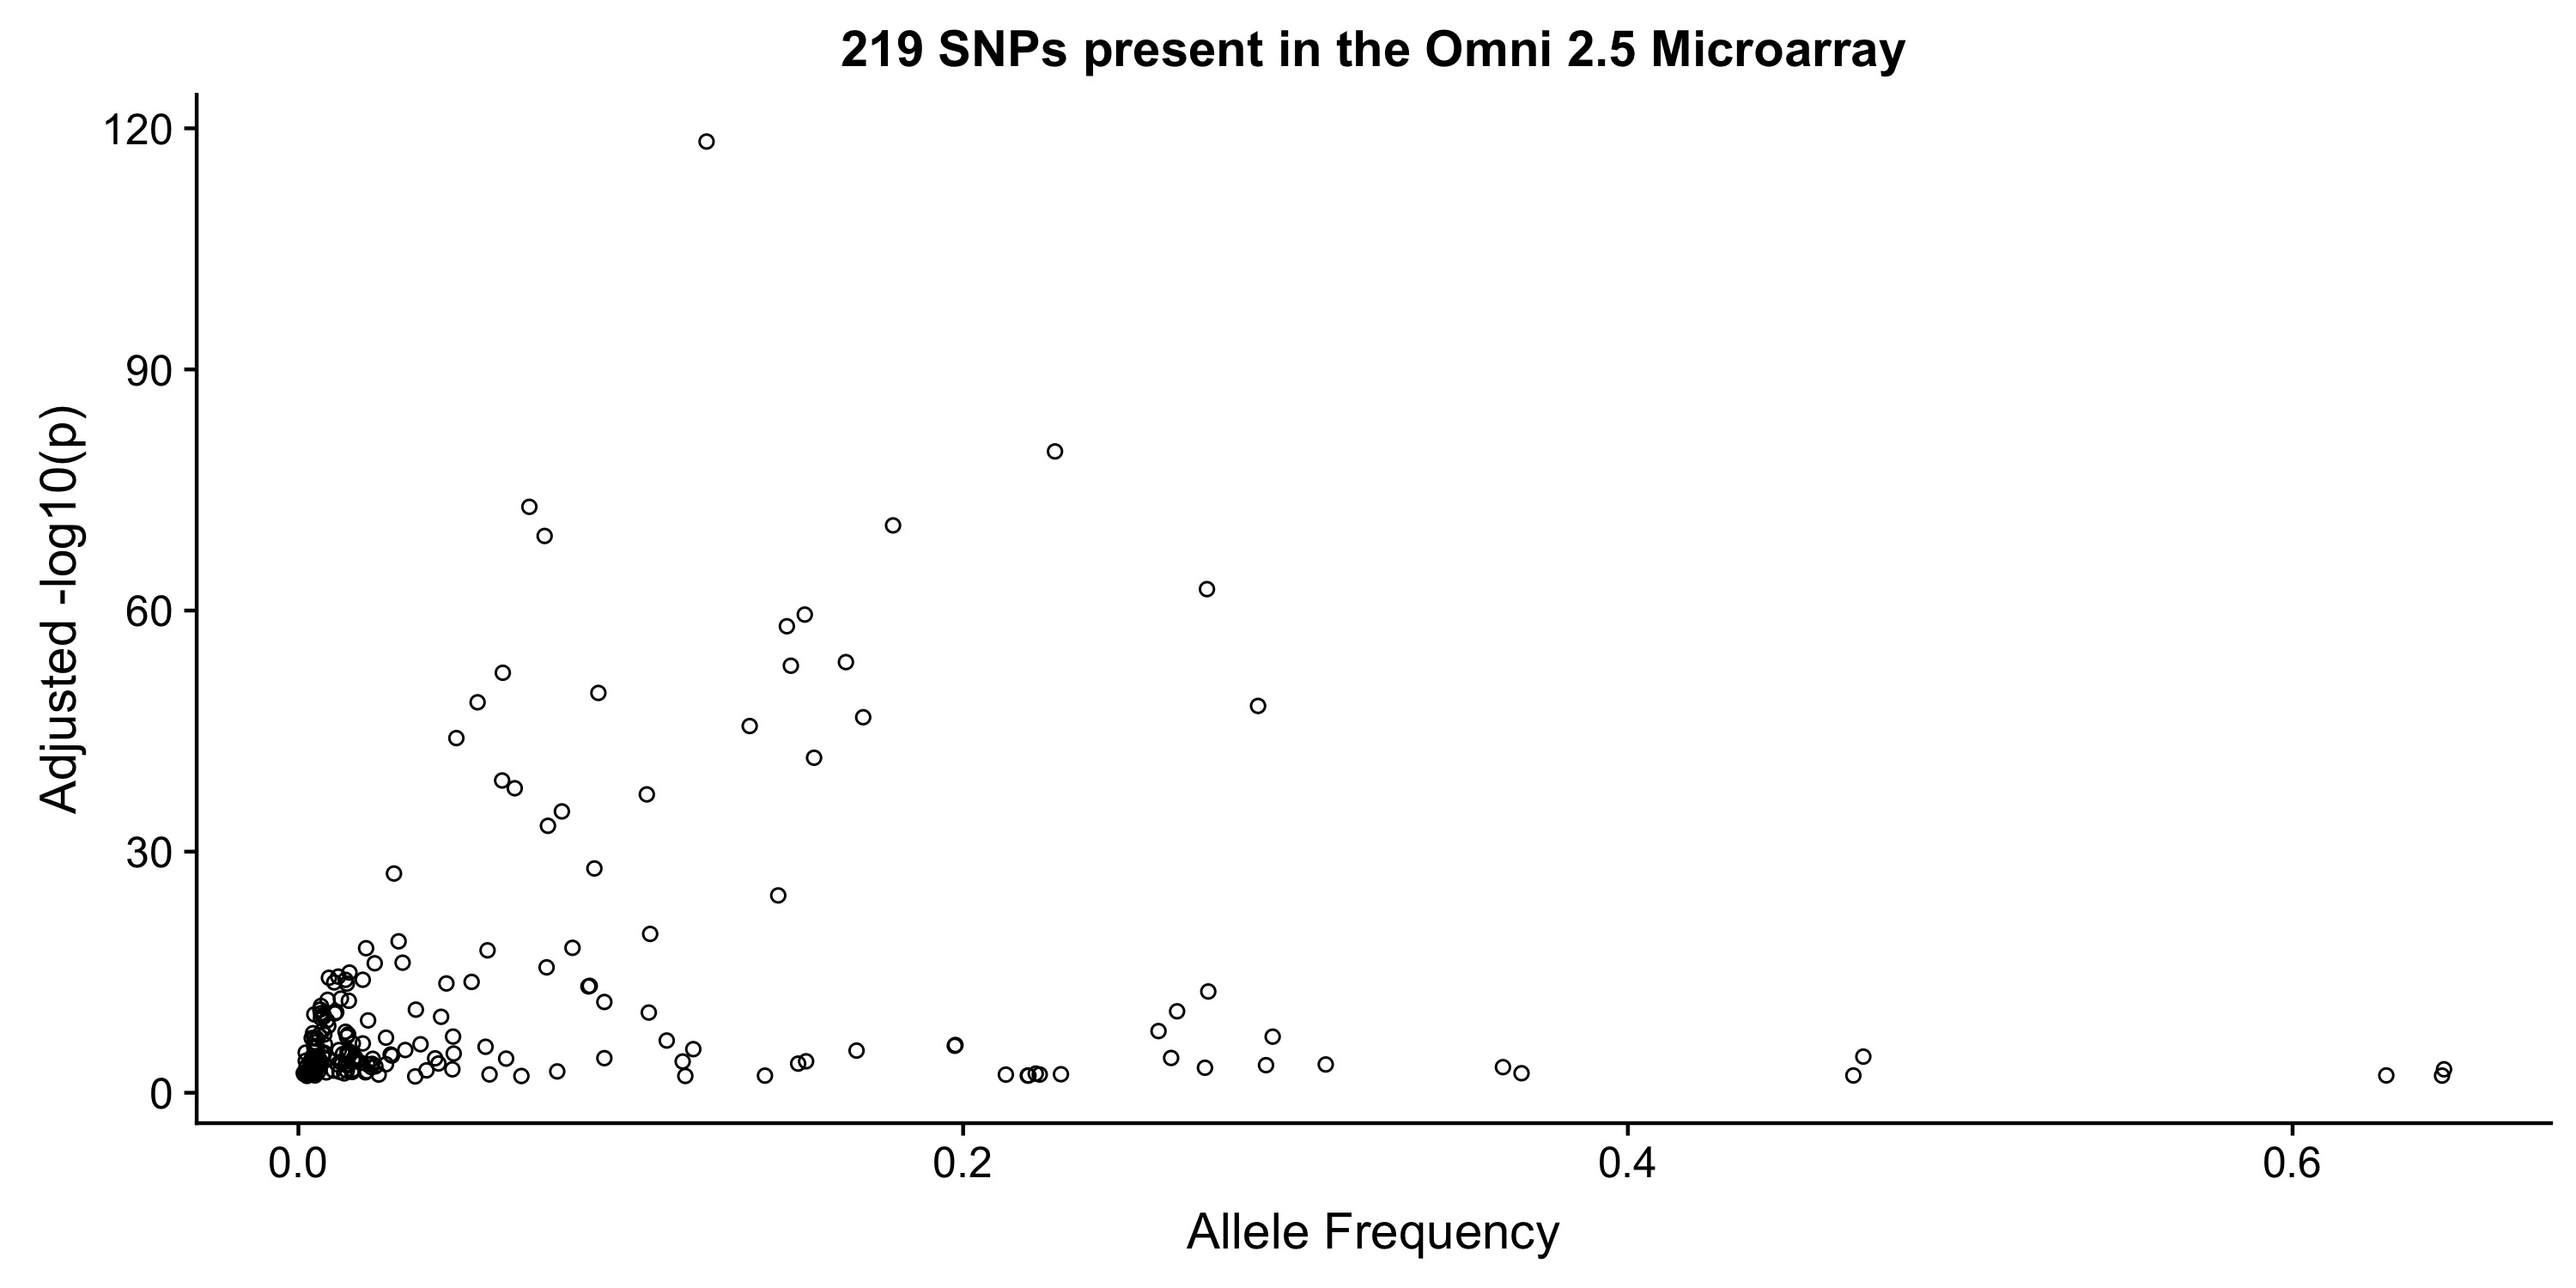
\includegraphics[width=12cm,keepaspectratio]{../Figures/Omni_AF.jpg}
\caption{Estimated frequency and association strength of $Q$- associated variants present on Illumina's Omni 2.5 chip. Variants highly associated to $Q$ tend to have low global allele frequencies.}
\label{Omni}
\end{figure}

\begin{figure}[ht]
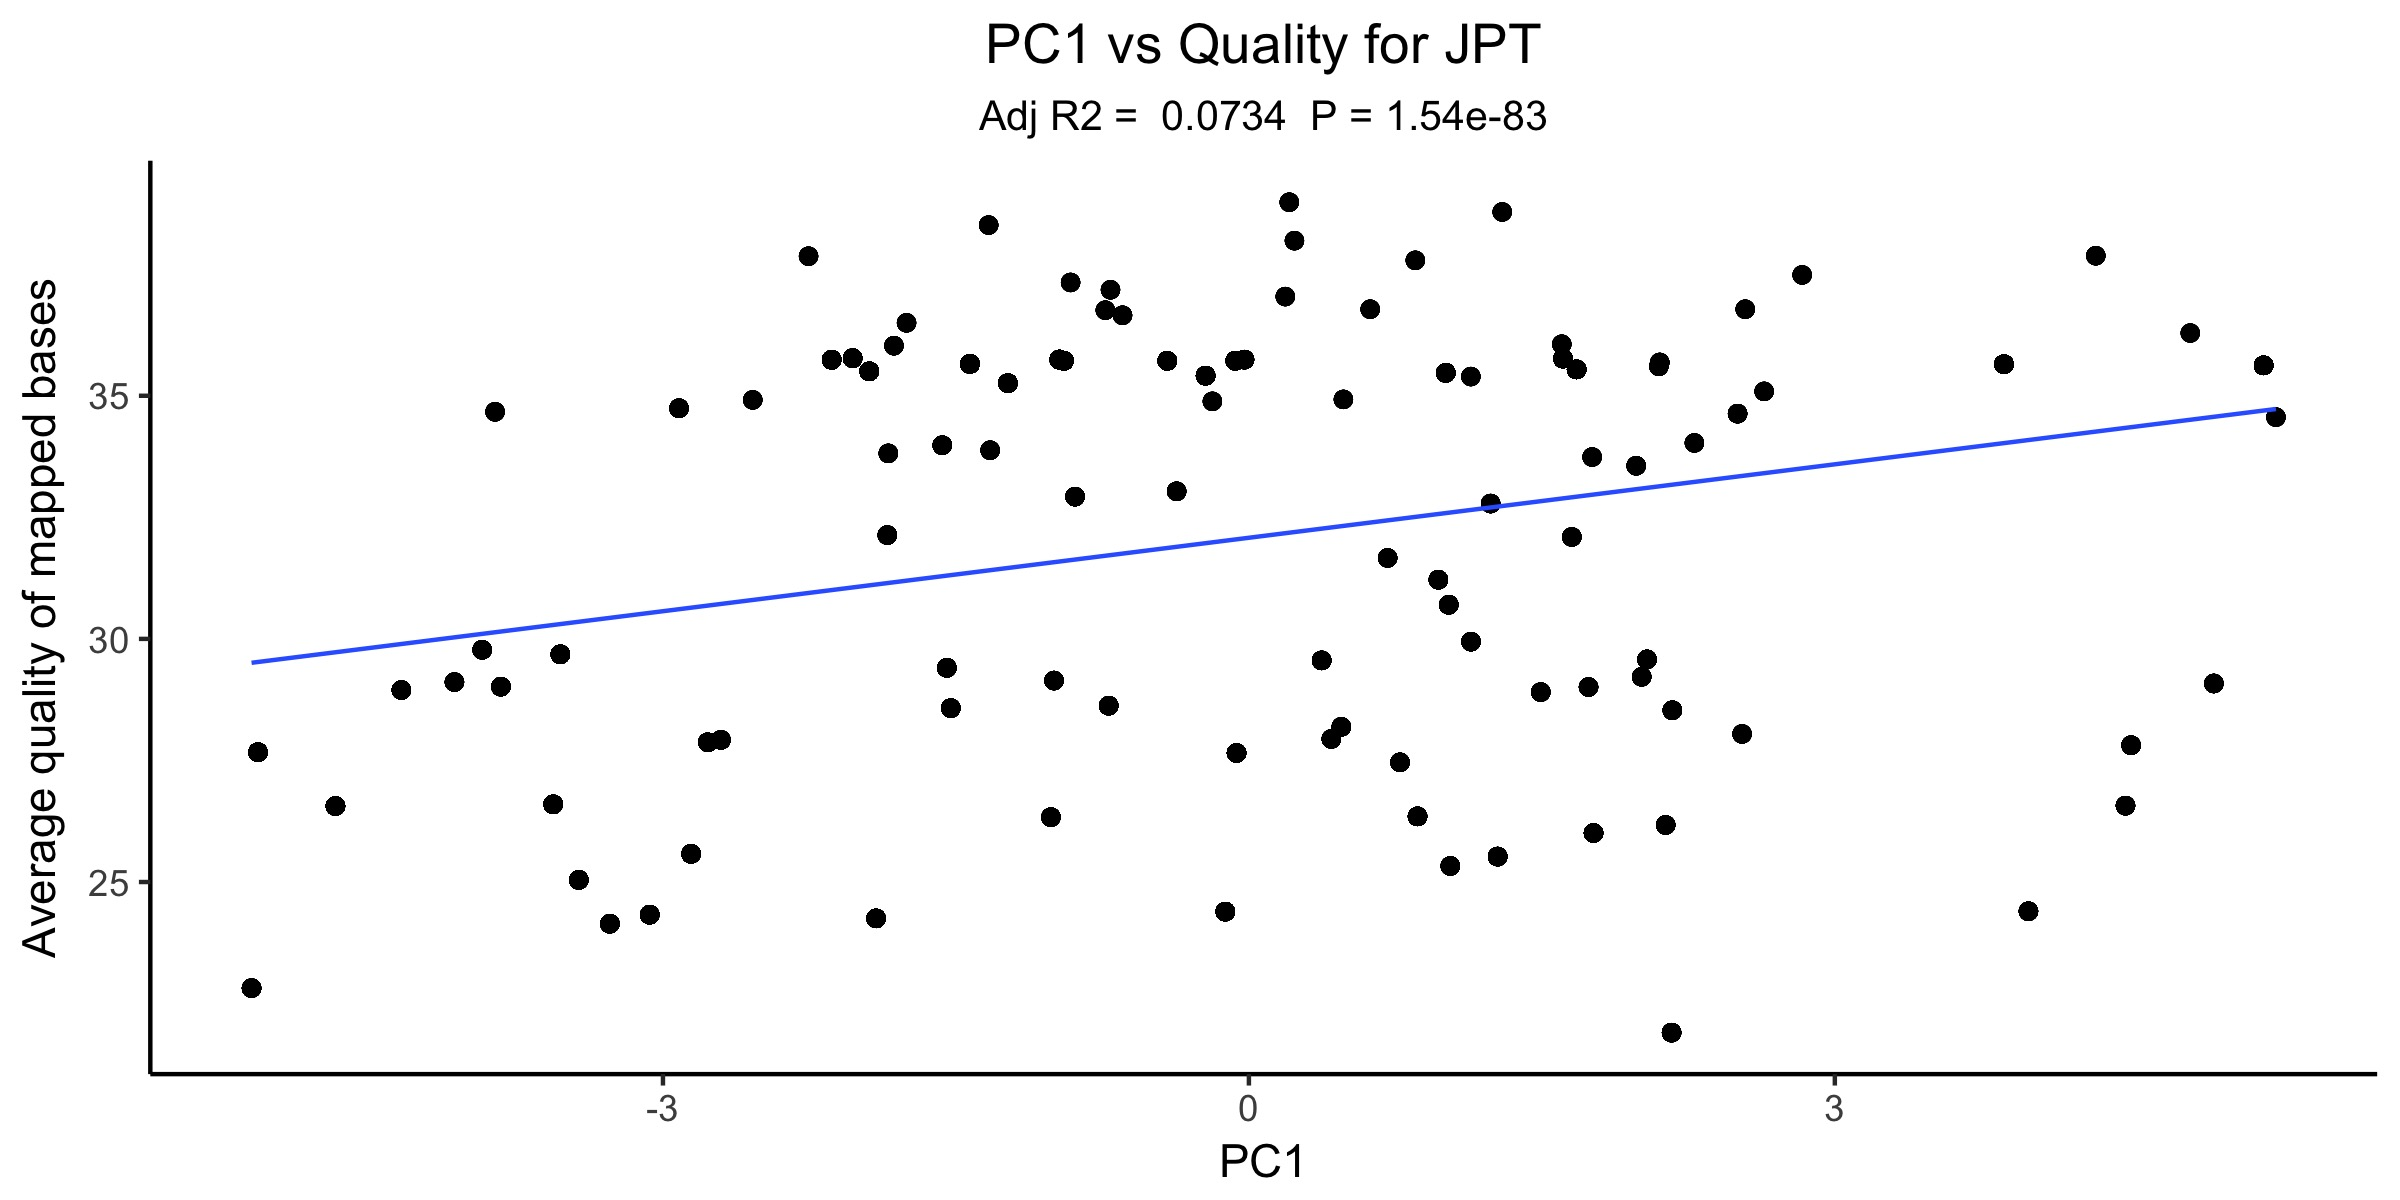
\includegraphics[width=12cm,keepaspectratio]{../Figures/PC1_Correlation.jpg}
\caption{Sequencing metrics against the prevalence of the  *AC${\rightarrow}$*CC mutational signature in 1000 Genomes Project. The average quality per mapped bases $Q$ per individual shows some clustering with individuals with low-quality data showing elevated rates of the signature.  }
\label{PC1_Correlation}
\end{figure}

\begin{figure}[ht]
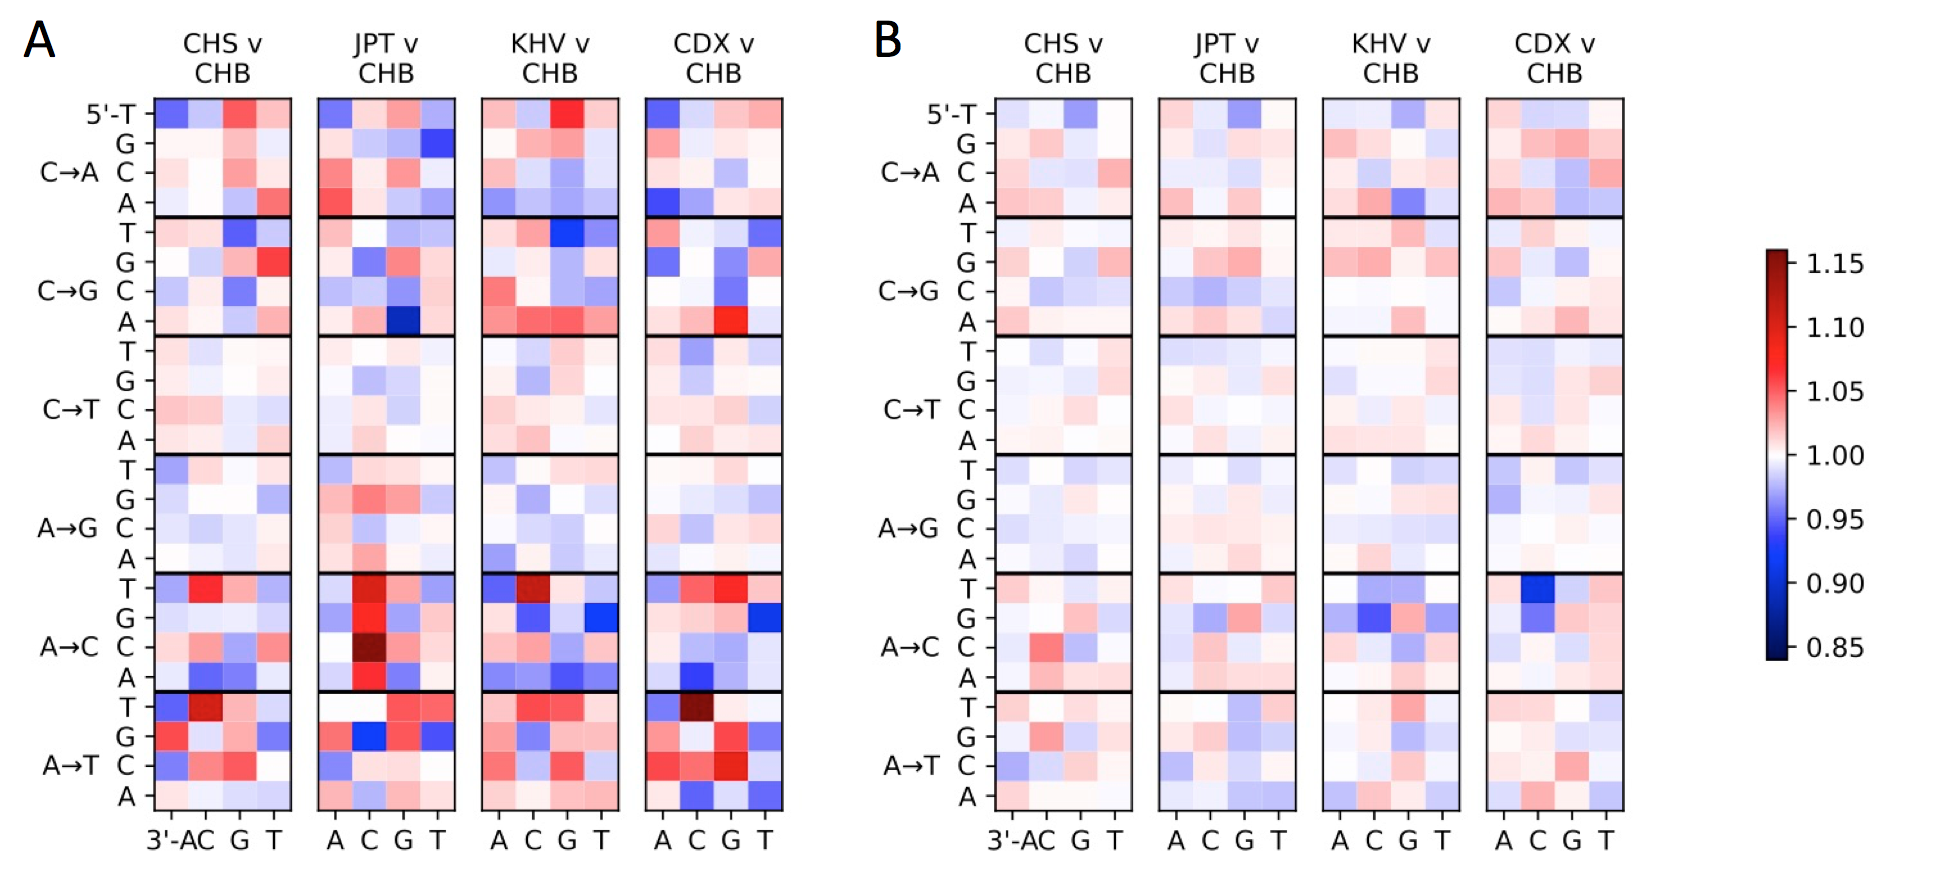
\includegraphics[width=12cm,keepaspectratio]{../Figures/MutationSpectrum_cutOff.png}

\caption{Comparing mutational signatures after removing $Q$-associated variants and after removing individuals with low $Q$.  \textbf{A} 
The  *AC${\rightarrow}$*CC mutational signature in JPT remains despite removing variants associated to quality.
\textbf{B} 
Removing individuals with average quality per mapped bases $Q$ below a threshold of 30 removes the mutational signature completely. }
\label{MutSpect}
\end{figure}


\end{document}
